\documentclass[11pt]{article}
\usepackage[margin=1in]{geometry} 
% For 1-inch margins
\usepackage{setspace}
\doublespacing % This command provides double-spacing

\usepackage{algorithmic} %For computer algorithm code in LATEX
\usepackage{algorithm} %For algorithm box around the algorithmic
\usepackage{float}
\usepackage{authblk}
\usepackage{amsmath,amsfonts,amssymb,amsthm}
\usepackage{bbm}
\usepackage{graphicx}
\usepackage{booktabs}
\usepackage{multirow}
\usepackage{enumitem}
\usepackage{xcolor}
\usepackage{hyperref}
\usepackage{natbib}
\bibliographystyle{apalike}
\usepackage{caption}
\usepackage{subcaption}





\captionsetup{width=0.9\textwidth,font={small}}


%% define theorems environment
\newtheorem{theorem}{Theorem}%  
\newtheorem{corollary}{Corollary}
\newtheorem{proposition}[theorem]{Proposition}%
\newtheorem{example}{Example}%
\newtheorem{lemma}{Lemma}%
\newtheorem*{remark}{Remark}

\newtheorem{definition}{Definition}
\newtheorem{assumption}{Assumption}






\newcommand{\E}{\mathbb{E}}
\newcommand{\R}{\mathbb{R}}
\newcommand{\ind}{\mathbbm{1}}
\newcommand{\pr}{\mathbb{P}}



\newcounter{stepcounter} 
\newenvironment{step}[1][] % Define with 1 optional argument, default is empty []
  {% Begin Step code
   \par\addvspace{\medskipamount}% Space before
   \refstepcounter{stepcounter}% Increment counter for numbering and referencing
   \noindent % Prevent paragraph indent
   \textit{% Start italics for the header
     Step \thestepcounter% Print "Step X"
     \def\@optarg{#1}% Temporarily store the optional argument
     \ifx\@optarg\@empty % Check if the optional argument #1 is empty
        % If empty, do nothing extra before the colon
     \else
        \space(#1)% If not empty, print a space and the argument in parentheses
     \fi % End of check
     .% Print the colon after number and optional title
   }% End italics for the header
   \quad % Add horizontal space after the italic header
   % --- User's step content follows here ---
  }%
  {% End Step code
   \par\addvspace{\medskipamount}% Space after
  }
\makeatother % Restore @ command behavior

% \title{Nonparametric Policy Learning under Spatial Confounding with Application in Groundwater Contaminants in Wisconsin}

\title{Safe, Cost-Effective Spatial Policy Learning With Applications to Groundwater Contamination in Wisconsin}



\author[1]{Xindi Lin}
\author[2]{Chan Park}
\author[3]{Christopher Zahasky}
\author[1]{Hyunseung Kang}

% \affil is the command for the affiliation
% Change the font size for all affiliations
\renewcommand{\Affilfont}{\small} 
% You can use any of the standard size commands:
% \tiny, \scriptsize, \footnotesize, \small, \normalsize,
% \large, \Large, \LARGE, \huge, \Huge

\affil[1]{Department of Statistics, University of Wisconsin-Madison}
\affil[2]{Department of Statistics, University of Illinois Urbana-Champaign}
\affil[3]{Department of Geoscience, University of Wisconsin-Madison}
\date{October 2025}

\begin{document}

\maketitle
% \textcolor{red}{A potential title: Safe, Cost-Effective Spatial Policy Learning With Applications to [Agricultural-Related Groundwater Contamination in Wisconsin]}
\begin{abstract}
    Environmental policies often aim to reduce contaminant level to a regulatory threshold. For example, when install water supply systems, the nitrate level has to be lower than the 10mg/L regulatory threshold. Increasing well depth of the water supply systems effectively decrease nitrate level but  incurs significant cost, the policymakers must therefore determine the minimum well depth required to meet the regulatory threshold. In this paper, we propose an optimal policy learning framework to identify the minimum treatment level needed at a given location to meet a given threshold. A key feature of our method is accounting for the spatial confounding and dependence. We estimate the optimal policy by empirical risk minimization with a novel, nonparametric, doubly robust loss function. We then characterize the statistical properties of the estimated policy in terms of the excess risk bound. We apply our method to design a safe, cost-effective nitrate mitigation policy for Wisconsin, aiming to decrease the nitrate level in drinking water to a given threshold.
\end{abstract}

\section{Introduction}


\subsection{Motivation}

For more than two decades, nitrate $(\mathrm{NO_3^{-}})$ has been one of the top three contaminants in drinking water supplies \citep{Pennino2017}. Excess nitrate in drinking water increases the risk of certain cancers and impacts fetal development during pregnancy \citep{Ward2005, USEPA1995a}. 
% Formed when nitrogen from fertilizers or other sources oxidizes, nitrate is highly water-soluble and does not adsorb well to soil particles. Consequently, it is easily transported into groundwater by precipitation and melting snow percolating through soil and bedrock.
Groundwater nitrate contamination can be especially high in areas with intense agricultural activities \citep{Nolan2002, Hudak2000, Spalding1993, Sobota2013, Sabo2018}, well-drained soils, and shallow water supply wells \citep{Glenn2010, Mueller1995, Enwright2009}. To protect against the health risks posed by nitrate, the U.S. Environmental Protection Agency (EPA) has established a standard of 10 mg/L for nitrate in drinking water, and the most effective intervention to decrease the nitrate level in water supply systems is increasing well depth to reach the safe water.

% \textcolor{red}{Safe but cost-effective policy}
However, the installation of deeper wells significantly increases costs, and the vast number of non-compliant wells makes universal intervention infeasible. The policymakers must therefore design cost-effective interventions that satisfy safety standards. This challenge motivates a constrained policy learning within spatial causal inference. Briefly, let $S_1,\ldots,S_n$ be a set of spatial locations. We seek an optimal policy function $\theta^*$, which maps site characteristics $X_i$ at location $S_i$ to a treatment level (well depth), such that the treatment intensity is minimized while ensuring the outcome remains below a safety threshold $\mathcal{T}$; a bit more formally:
\begin{equation}\label{eq:brief}
    \theta^*(X_i)=\arg \min_{\theta\in\Theta} \theta(X_i) \quad\text{subject to}\quad \mathcal{Y}(\theta(X_i))\leq \mathcal{T} \quad\text{for all}\quad i = 1,\ldots,n.
\end{equation}
\noindent
Here, $\Theta$ represents the class of candidate policies, and $\mathcal{Y}(\theta(X_i))$ denotes the expected potential outcome (nitrate level) at location $S_i$ under the policy-prescribed depth $\theta(X_i)$. The optimal policy $\theta^*$ identifies the minimum well depth required to guarantee compliance with the safety threshold $\mathcal{T}$. This formulation for learning a safe, cost effective policy against strict regulatory thresholds extends beyond groundwater nitrate to a general class of environmental problems. Contaminants such as PM2.5 \citep{esworthy2013air} and PFAS \citep{park2024statistical} present identical challenges: effective interventions are available but financially demanding, requiring policymakers to balance cost minimization with compliance thresholds.


\subsection{Prior Work}

% \textcolor{red}{list all every prior work}

The problem is closely related to policy learning for individualized treatment regimes; for example, \citet{Richter1999, Laber2018, Ren2022} incorporate treatment costs into optimal allocation policies. In the context of continuous treatments, \citet{chen2016personalized} derive optimal individualized dose rules (IDR) to maximize clinical benefits, while \citet{chen2022policy, park2023personalized} focus on identifying effective dosage ranges to achieve specific potential outcome targets. Similarly, \citet{park2024minimum} address the minimization problem in \eqref{eq:brief} for binary treatments within multilevel studies under partial interference. However, the validity of these methods typically relies on two key assumptions: (i) unconfoundedness (no unmeasured confounders) and (ii) independent and identically distributed (i.i.d.) observations. These assumptions are frequently violated in environmental observational data. 
\cite{Athey2018} learn a treatment assignment policy under constraints constraints by framing the problem as a weighted classification problem using doubly robust scores. 


% \textcolor{red}{add new paper about constrained policy learning that Ren(2022), multi-objective policy learning}

% \textcolor{red}{literature review of method/(scientific paper tha potentially applied). At the beginning of prior work}

When the unconfoundedness assumption is violated, a common strategy is to use spatial coordinates as a proxy for unmeasured confounders, assuming these confounders possess spatial structure. A standard approach is the spatial linear mixed model $Y(S) = \beta^\top X(S) + U(S)+\epsilon(S)$
% \begin{equation}\label{eq:linear mixed effect}
%     Y(S) = \beta^\top X(S) + U(S)+\epsilon(S)
% \end{equation}
where $X(S)$ denotes the measured covariates or treatment, $\beta$ is the target parameter, $\epsilon(S)$ is i.i.d. random error, and $U(S)$ captures the unmeasured spatial confounders \citep{thaden2018structural,dupont2022spatial+,wiecha2024two,datta2025consistent,burman2025robust,gilbert2024consistency}; Furthermore, \citet{gilbert2021causal} provide sufficient conditions for the nonparametric identification of continuous exposure effects in the presence of such spatial confounding.

% \textcolor{red}{different conditions of U(S) and X(S) } consider the consistent estimation 

% \textcolor{red}{there is no existing work of policy learning in the presence of spatial confounding, also we make weaker assumption, not only identity the policy, but estimate policy}


When the i.i.d. assumption does not hold, Gaussian processes (GPs) are frequently employed to model the dependence structure. In geospatial machine learning, this often takes the form of a nonparametric mixed-effects model, $Y(S) = m(X(S)) + U(S) + \epsilon(S)$, where $m(\cdot)$ represents the target function and $U(S)$ is a Gaussian process. Recent works by \citet{sigrist2022gaussian, saha2023random, zhan2024neural} adapt  gradient boosting, random forests, and neural networks, respectively, to estimate the nonparametric component $m(\cdot)$ in the mixed-effects model, often coupling these with kriging \citep{cressie2015statistics} to estimate the GP component $U(S)$. In the causal inference domain, \citet{gilbert2021causal} extend the double machine learning framework \citep{colangelo2025double, chernozhukov2018double} to spatially dependent data, assuming weak dependence.

% Georgia's paper (interference related paper, zigler, Gergia, francesca, Laura)

% double machine learning in dependent paper. 



\subsection{Our contribution}

Our work builds on an earlier work by \citet{park2024minimum} estimating the policy in \eqref{eq:brief} within the context of multi-level studies with binary treatment. Specifically, we extend \citet{park2024minimum} to identify, estimate, and theoretically characterize the safe, cost-effective policy $\theta^*$ for continuous treatments in the presence of spatial confounding, and dependence. This extension necessitates three distinct innovations. First, the presence of spatial confounding requires new causal identification conditions tailored to environmental observational studies (Section \ref{sec:identify_spatial_confounding}). Second, we propose a new outcome regression strategy based on geospatial machine learning (Section \ref{section:outcome_regression}) to handle spatial dependence. Third, the continuous treatment setting requires a new risk minimization method incorporating kernel smoothing (Section \ref{sec:direct_method}). Furthermore, our theoretical analysis explicitly quantifies the impact of spatial dependence and kernel smoothing on the excess risk (See Section \ref{sec:theory}). In contrast, \citet{park2024minimum} assumes unconfoundedness and i.i.d. observations for binary treatment, which enable the use of standard double machine learning estimator and theoretical analysis.



The rest of the paper is organized as follows. Section \ref{sec:setup} discusses the identifying $\theta^*$ in the presence of spatial confounding. Section \ref{sec:estimator} discusses estimating $\theta^*$ based on a nonparametric, empirical
risk minimization problem with a doubly robust loss function. Section \ref{sec:simulation} applies the proposed method to simulated data and Section \ref{sec:application} uses the proposed method to design a safe, cost-effective nitrate policy in Wisconsin.



\section{Setup}\label{sec:setup}

\subsection{Notation}
 To define causal parameters under spatial confounding, we adopt the potential outcomes framework \cite{rubin1974estimating}. Let $\mathcal{S} = \{S_1,S_2,\ldots,S_n\} $ represent the set of $n$ distinct spatial locations within a domain $\mathcal{D} \subset \mathbb{R}^2$. For each location $S_i\in\mathcal{S}$, we let $Y_i$ be the observed outcome, $A_i\in \mathcal{A}=[a_L,a_U]$ be the observed  treatment level whose range has the lower and upper bounds ($a_L$ and $a_U$), $Y_i(a)$ be the potential outcome, $X_i$ be the observed covariates, and $U_i$ be the unmeasured spatially-varying confounders. We use $\mathcal{T}$ to denote the target threshold of the potential outcome. Given any location $S_0\in\mathcal{D}$, and let $Y_0,Y_0(a),X_0,U_0$ be the corresponding variables, we define the optimal policy at $S_0$ as the minimum level of treatment such that the conditional expectation of the potential outcome achieves the threshold $\mathcal{T}$ as follows:
\begin{equation}\label{eq:def_estimand}
    \theta^*(S_0) = \arg\min_{a\in\mathcal{A}} \ a, \ \text{such that } \E[Y_0(a)| X_0, U_0]\leq \mathcal{T}.
\end{equation}
\noindent In the nitrate example, $\mathcal{S}$ is the set of locations of drinking water wells. For each well location $S_i$, $Y_i$ is the measured nitrate level, $Y_i(a)$ is the nitrate level if the well were to have depth $a$, $X_i$ is the covariate associated with the nitrate level in groundwater,  $U_i$ is the spatially varying trend of nitrate that cannot be captured by $X_i$, and $\mathcal{T}$ is the nitrate enforcement standard set by the EPA, $\theta^*(S_0)$ in \eqref{eq:def_estimand} is the minimum well depth such that the expectation of nitrate level in the well drilled at $S_0$ reaches the enforcement standard. 

\subsection{Identification}\label{sec:identify_classic}

Let $\Theta = \big\{ \theta \big| \theta(S_0) \in [a_L,a_U] \}$ be a collection of functions from the study region $\mathcal{D}$ to the treatment range $[a_L,a_U]$. 
A function $\theta \in \Theta$ is one possible policy that outputs the minimum depth the well should be drilled at $S_0$. To identify the optimal policy $\theta^*$ defined in \eqref{eq:def_estimand}, we first make the following assumptions
 \begin{enumerate}[label=(A\arabic*)]
     \item Causal consistency:  $Y_i = Y_i(A_i)$ almost surely. \label{condition:consistency}
        \item Conditional Ignorability/Unconfoundedness: $A_i \perp Y_i(a) \mid X_i, U_i .$ \label{condition:ignorability}
        \item Overlap: $p(a \mid X_i=x, U_i=u) > 0 \text{ for all a, x, u almost surely}$. \label{condition:overlap}
 \end{enumerate}

 The causal consistency assumption \ref{condition:consistency} is the fundamental assumption in causal inference, implying that the potential outcomes are well defined in $\mathcal{D}$.
Assumptions \ref{condition:ignorability} - \ref{condition:overlap} are natural extensions of conditional ignorability,
and overlap from the classic i.i.d. setting to spatial confounders in spatial causal inference literature (e.g., \cite{papadogeorgou2019adjusting, schnell2020mitigating, gilbert2021causal}). Under Assumptions \ref{condition:consistency} - \ref{condition:overlap}, we can identity the conditional expectation of the potential outcome in \eqref{eq:def_estimand} if $U_i$ is observed, i.e., 
\begin{equation}\label{eq:identification_1}
    \E[Y_0(a)| X_0 = x_0,U_0 = u_0] = \E[Y_0| A_0 = a, X_0 = x_0,U_0 = u_0]
\end{equation}


\subsection{Identification under Spatial Confounding}\label{sec:identify_spatial_confounding}
In the presence of spatial confounding, i.e., $U_i$ in Assumptions \ref{condition:ignorability} - \ref{condition:overlap} is unmeasured, Assumptions \ref{condition:consistency} - \ref{condition:overlap} is insufficient for the identification of \eqref{eq:def_estimand}. Fortunately, when $U_i$ varies spatially with the observed location $S_i$, using $S_i$ as a proxy may mitigate the confounding issue, which is strategy taken by nearly all methods for spatial confounding in the literature, see \citet{gilbert2021causal,wiecha2024two, gilbert2024consistency}. To this end, we assume two additional assumption under which we can replace $U_i$ in the right-hand side of \eqref{eq:identification_1} by $S_i$, 
  \begin{enumerate}[label=(A\arabic*), start=3]
\item $U_i = g(S_i)$ for a fixed function $g$ that is continuous almost surely.\label{condition:smooth_spatial_confounder} 
 \end{enumerate} 
Assumption \ref{condition:smooth_spatial_confounder} requires that the unmeasured confounders are determined by location, and is almost surely continuous over the space. In the nitrate example, this assumption is generally satisfied if the unmeasured confounder $U$ is a hydrogeological feature, such as the static water level. Conversely, Assumption \ref{condition:smooth_spatial_confounder} may be violated if $U$ is not determined solely by spatial coordinates (e.g., well usage, where wells at the same location serve different purposes) or if $U$ is spatially discontinuous (e.g., categorical variables like land use). Therefore, to identify the causal effect of well depth, we must observe all confounders that are either not strictly functions of space or are spatially discontinuous."

% On the other hand, Assumption \ref{condition:smooth_spatial_confounder} can fail to satisfied in two ways. First, $U$ may not be function of space alone. For example, considering well usage as a potential confounder. Wells  at the same location might have different well usage (e.g., private potable wells versus public municipal wells), meaning $U$ is not determined solely by its spatial coordinates. Second, even if $U$ is a function of $S$, it is not necessarily a continuous function of $S$. For example considering land use as a potential unmeasured confounders. While land use is uniquely determined by the spatial coordinates, it is a categorical variable and inherently discontinuous. 


% Therefore, to identify the causal effect of well depth, we must observe all confounders that are either not solely a function of space or are spatially discontinuous.

Then, we make the following assumption that conditioning on $S$ does not induce confounding:
  \begin{enumerate}[label=(A\arabic*), start=4]
\item $ Y_i(a)\perp A_i\mid X_i, U_i,S_i$. \label{condition:no_confouning_spatial_confounder_weak}
 \end{enumerate} 

 \begin{figure}
    \centering
    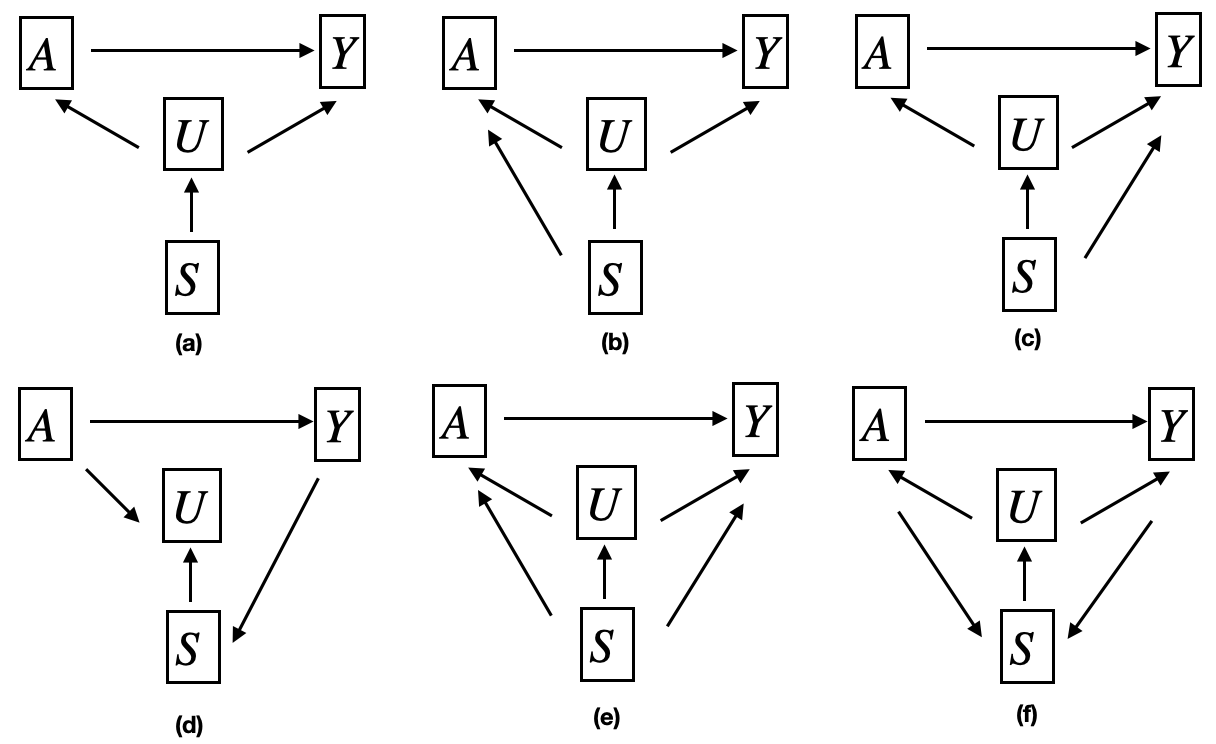
\includegraphics[width=0.9\linewidth]{causal_DAG.png}
    \caption{Causal DAGs illustrating unconfoundedness conditional on spatial location. The measured confounder $X$ is omitted for clarity. Panels (a)–(c) show scenarios where the identification assumptions are satisfied, while panels (d)–(f) show scenarios where the assumptions are violated.}
    \label{fig:causal_DAG}
\end{figure}
 
Assumption \ref{condition:no_confouning_spatial_confounder_weak} generally holds when the spatial location $S$ is a parent of the nitrate level $Y$ and well depth $A$ (as illustrated in cases (a), (b), (c), and (e) of Figure \ref{fig:causal_DAG}). Conversely, this assumption is violated if $S$ acts as a collider or a descendant of a collider (cases (d) and (f) in Figure \ref{fig:causal_DAG}). Additionally, while case (e) in Figure \ref{fig:causal_DAG} satisfies Assumption \ref{condition:no_confouning_spatial_confounder_weak}, it violates Assumption \ref{condition:ignorability}.

In the nitrate example, we assume a specific structure that aligns with case (a). We assume that the spatial location itself is not a direct cause of the nitrate level $Y$ or the well depth $A$. Instead, $S$ influences both $Y$ and $A$ indirectly through unobserved geographical features (such as aquifer and additional soil properties). This scenario motivates a stronger, more intuitive assumption:  
   \begin{enumerate}[label=(A\arabic*), start=5]
\item $ (Y_i(a), A_i)\perp S_i\mid X_i, U_i$. \label{condition:no_confouning_spatial_confounder_strong}
 \end{enumerate} 
This specifies that once the true unobserved spatial confounders $U$ and the observed covariates $X$ are accounted for, the location $S$ provides no remaining information about the potential outcomes or the treatment. 


\begin{proposition}\label{prop:identification}
    Let $\mu^*(a,x,s):=E[Y|A=a, X = x, S = s]$. Under Assumption \ref{condition:consistency} - \ref{condition:no_confouning_spatial_confounder_weak}, $\theta^*$ can be identified by
        \begin{equation}\label{eq:identification}
            \theta^*(S_0) = \arg\min_{a\in\mathcal{A}} \ a, \ \text{such that } \mu^*(a,X_0,S_0)\leq \mathcal{T}.
        \end{equation}
\end{proposition}
\noindent We remark that Assumption \ref{condition:consistency} - \ref{condition:no_confouning_spatial_confounder_weak} are sufficient nonparametric identification assumptions allowing us to express the counterfactual estimand \eqref{eq:def_estimand} as the statistical functional \eqref{eq:identification}. In settings where causal inference is not the primary goal and the objective is to estimate \eqref{eq:identification}, these assumptions are not required and the estimation approach proposed in the subsequent section remains valid. 


% \noindent 
Lastly, we make the following monotonicity assumption for the outcome regression.
  \begin{enumerate}[label=(A\arabic*), start=6]
        \item Monotonicity: $\mu^*(a,x,s)$ is monotonically decreasing in $a$ for any $x$, $s$, and $\mu^*(a_U,x,s)\leq \mathcal{T}$. \label{condition:monotonicity}
 \end{enumerate}
Assumption \ref{condition:monotonicity} implies that the expectation of the potential outcome decrease with the treatment, and the upper bound of the treatment is guaranteed to achieve the target threshold $\mathcal{T}$. In practice, Assumption \ref{condition:monotonicity} is plausible if the treatment is used to reduce the level of the  outcome and the treatment range is wide enough. Alternative to assuming $\mu^*(a_U,x,s)\leq \mathcal{T}$ for all $x$ and $x$, we can extend the definition \eqref{eq:def_estimand} to let $\theta^*(S_0)=a_U$ if $\mu^*(a_U,X_0,S_0)>\mathcal{T}$ at a location $S_0$. In the nitrate example, the nitrate in groundwater is originally from nitrogen (N) from surface land. As nitrogen converts to nitrate, it dissolves in water and gradually seeps into groundwater by rain. Thus, it is scientifically reasonable to assume \ref{condition:monotonicity}, i.e, increasing the well depth can decrease the nitrate level. Of note, the direct approach relies on Assumption \ref{condition:monotonicity} to make the optimal policy $\theta_0$ in \eqref{eq:def_estimand} as the global minimum of the proposed risk function (see Lemma \ref{lemma:risk_db} below for details). In contrast, the indirect approach remains applicable for estimating the optimal policy $\theta^*$.




% \textcolor{red}{What if (A1)-(A4) are not valid, we do not have causal identification, but if equation (4) is the objective function of the interest, then the subseuqent is still vaid to solve the estimating problem.}




\section{Estimation}\label{sec:estimator}

\subsection{An Indirect Method Via Geospatial Machine Learning}\label{sec:indirect_method}

We first present a naive  estimator of $\theta^*$ based on indirectly using the spatial modeling of the observed outcome. This is sometimes referred to as ``indirect'' method in the classic non-spatial setting \citep{chakraborty2013statistical}; see \citet{Deliu2022} for a recent review. Formally, let $\hat\mu$ be an estimator of $\mu^*$ in Proposition \ref{prop:identification}. Then, under Assumptions \ref{condition:consistency} - \ref{condition:no_confouning_spatial_confounder_weak}, an estimator of $\theta^*(S_0)$ is obtained by replacing $\mu^*$ with $\hat\mu$ in \eqref{eq:identification} and doing a grid search over the range of the treatment:
$$\hat{\theta}(S_0)=\inf_{a\in\mathcal{A}}\left\{a \mid \hat\mu(a,X_{0},S_0)\leq \mathcal{T}\right\}.$$
\noindent
We again remark that Assumption \ref{condition:monotonicity} is not necessary for the indirect approach. However, a notable limitation of this indirect approach is its heavy reliance on a correctly specified and well-estimated outcome regression model. Compare to standard i.i.d. data, it is substantially more challenging to obtain a consistent nonparametric estimator for $\mu^*$ in the presence of spatial confounding; see Section \ref{section:outcome_regression}. Also, similar to \citet{Zhao2012} observation about the indirect approach under non-spatial i.i.d. setting, our indirect approach may have poor finite-sample properties compared to an approach that directly estimates $\theta^*$. 
% In our simulation study in Section \textcolor{red}{xxx}, we reconfirm this observation under spatial confounding setting and, consequently, we recommend the direct approach for estimating $\theta^*$.

\subsection{Outcome Regression Based on Geospatial Machine Learning}\label{section:outcome_regression}

Unlike the standard i.i.d. setting where the outcome regression model can be estimated with a wide range of nonparametric estimator  \citep{Nadaraya1964, Watson1964, Breiman2001,goodfellow2016deep,hastie2017generalized}, it is infeasible to use spatial co-ordinates or some transformations (like distances or basis functions) as additional covariates and apply a nonparametric machine learning estimator \citep{hengl2018random, chen2020deepkriging, gray2022use} to estimate $\mu^*$ in \eqref{eq:identification} in the presence of spatial confounding. The flexibility of such estimator can leads to overfitting to the spatial co-ordinate and violate the smoothness of unmeasured spatial confounder $U_i$ in Assumption \ref{condition:smooth_spatial_confounder}. Therefore, instead of adding spatial co-ordinates as additional covariate, we adopt a nonparametric spatial mixed effect model, a framework that has been successfully integrated with modern geospatial machine learning methods in recent literature \citep{sigrist2022gaussian,saha2023random, zhan2024neural}. For the observed spatial data, we assume the following model:
\begin{equation}\label{eq:spatial_mixed_effect_model}
    Y_i = f(A_i,X_i) + U_i +\epsilon_i, \quad  \forall S_i\in\mathcal{D}.
\end{equation}
 Here, $f(A_i,X_i)$ is a nonparametric function of the treatment level $A_i$ and observed covariate $X_i$ that can be estimated by a wide-range of machine learning method. $U_i$ is a GP-distributed random effect with a parametric covariance function $C(\cdot;\psi)$, and $\epsilon_i$ is i.i.d. random gaussian error. This model leverages the advantages of both machine learning and GP framework. Specifically, the nonparametric $f(A_i,X_i)$ allows the interaction and non-linearity of the treatment and observed covariates. The GP-distributed $U_i$ provides a flexible modeling of the unmeasured confounder effect while maintain an implicit control of the smoothness by the covariance function of GP (e.g. the smoothness parameter of the Matern covariance function). Furthermore, the GP framework is computationally scalable on large scale spatial dataset using methods like Vecchia approximation \citep{vecchia1988estimation, datta2016hierarchical, katzfuss2021general}.

Assuming a nonparametric spatial mixed effect model in \eqref{eq:spatial_mixed_effect_model}, our estimation framework of the outcome regression is stated below.
\begin{step}[Initial Regression]\label{step:regression}Apply machine learning method to fit $Y_i$ on $A_i$ and $X_i$ to obtain the estimate $\hat f(a,x)$.
\end{step}

\begin{step}[GP Covariance Estimation]\label{step:covariance_estimation}Denote $\hat U_i=Y_i - \hat f(A_i,X_i)$, $\hat{\mathbf{U}} =(\hat U_1,\cdots,\hat U_n)$. $\mathbf{C}(\psi) = \{C(\|S_i-S_j\|;\psi)\}_{i,j=1}^n$. Obtain $\hat\psi$ by maximum-likelihood estimation:
            $$\hat\psi = \arg\max_{\psi}\left\{-\frac{n}{2}\log(|\mathbf{C}(\psi)|)-\frac{1}{2}\sum_{i=1}^n \hat{\mathbf{U}}^\top\mathbf{C}(\psi)^{-1}\hat{\mathbf{U}}\right\}$$
            
\end{step}

\begin{step}[Kriging]\label{step:kriging}For any location $S_0\in\mathcal{D}$, we let $\mathcal{S}_{-0}:=\mathcal{S}\backslash S_0$ be the set of locations with observations excluding $S_0$. We let $\hat{\textbf{U}}_{-0}$ be the fitted residual, $\mathbf{C}_{-0}(\psi)$ be the covariance matrix on $\mathcal{S}_{-0}$, and let $\mathbf{C}_{0}(\psi)$ be the vector of the covariance between $S_0$ and $\mathcal{S}_{-0}$. Then, we define 
$$\hat\E[U_0|\textbf{U}_{-0}] = \mathbf{C}_{0}(\hat\psi)\mathbf{C}^{-1}_{-0}(\hat\psi)\hat{\textbf{U}}_{-0}.$$
The estimated outcome regression is $\hat\mu(a,X_0,U_0) = \hat f(a,X_0)+\hat\E[U_0|\textbf{U}_{-0}].$
\end{step}

\begin{remark}
    When nonparametrically estimating the function $f(\cdot,\cdot)$ in Step \ref{step:regression}, standard machine learning method that rely on an Ordinary Least Squares (OLS) loss function are known to be inconsistent in the presence of spatial confounding \citep{gilbert2024consistency}. Thankfully, recent works have shown that employing a Generalized Least Squares (GLS) approach that accounts for the spatial correlation in $U_0$ yields a consistent estimator of $f(\cdot,\cdot)$ for parametric models \citep{gilbert2024consistency, datta2025consistent}. Formal consistency proofs to estimate $f(\cdot,\cdot)$ using a GLS-based machine learning method \citep{sigrist2022gaussian,saha2023random, zhan2024neural}.
% We also note that when $U_i$ is independent with $A_i,X_i$, i.e., only spatial dependence, no spatial confounding, both OLS-machine learning and GLS-machine learning can obtain consistent estimator of $f(\cdot,\cdot)$ but the GLS-machine learning estimator will be more efficient.
We note that it is important to distinguish this from the case of spatial dependence without confounding (i.e., when $U_i$ is independent of $A_i$ and $X_i$). In that scenario, both OLS-based and GLS-based machine learning estimators are consistent. However, the GLS-based estimator remains advantageous, as it will be more statistically efficient; see \citep{sigrist2022gaussian,saha2023random, zhan2024neural} for details.
\end{remark}




\subsection{A Direct Method Via Risk Minimization}\label{sec:direct_method}

In this section, we propose our preferred estimation approach based on directly estimating the optimal policy. We do this by recasting $\theta_0^*$ as a solution to risk minimization problems with specialized doubly robust loss functions. Notably, by reframing the original problem as a risk minimization problem, we can specify the class of policy as a function of the covariates and leverage a wealth of methods in empirical risk minimization to directly obtain estimators of $\theta^*$.

Formally, for $a\in[a_L,a_U]$, let $p^*(a|X_i,S_i)$ be the generalized propensity score, i.e., the conditional density of observed treatment level $A_i$ given the measured covariates $X_i$ and spatial coordinates $S_i$. Let $K_\delta(\cdot)$ be a scaled-kernel function with bandwidth $\delta$. Let $O_i:=\{A_i,X_i,S_i,Y_i\}$. For a given observation $O_i$ and treatment level $a$, we define the loss function $L^{(\delta)}(a,O_i)$ as follows:
\begin{subequations}\label{eq:loss_function_complete}
    \begin{equation}
        L^{(\delta)}(a,O_i) = \begin{cases}\label{eq:loss_function_real_line}
    \nu^{(\delta)}(a_L, O_i)+\epsilon -\epsilon \left\{\log( e + a_L- a)\right\}^{-1}& \text{if } -\infty<a<a_L\\
    \nu^{(\delta)}(a, O_i)&\text{if }  a_L\leq a\leq a_U\\
    \nu^{(\delta)}(a_U, O_i)+\epsilon -\epsilon \left\{\log( e + a- a_U)\right\}^{-1}&\text{if }  a_U<t< \infty
\end{cases}
    \end{equation}
    \begin{equation}\label{eq:loss_function_bounded}
        \nu^{(\delta)}(a, O_i) = \int_{\mathcal{A}} (\mathcal{T} - \psi^{(\delta)}(a^\prime,O_i))1(a^\prime\leq a)\mathrm{d}a^\prime + C_0.
    \end{equation}
\begin{equation}\label{eq:pseudo_outcome}
    \psi^{(\delta)}(a,O_i) := \mu(a,X_i,S_i)+ \frac{(Y_i - \mu(A_i,X_i,S_i))K_\delta(A_i-a)}{p(A_{i}|X_{i},S_{i})}.
\end{equation}
    
\end{subequations}

\noindent This loss function is constructed in a piecewise manner, as shown in \eqref{eq:loss_function_real_line}. Within the treatment range $a \in [a_L,a_U]$, the loss function is equal to $\nu^{(\delta)}(a, O_i)$. Outside the treatment range, $L^{(\delta)}(a,O_i)$ is strictly decreasing over $a \in (-\infty,a_L)$ and increasing over $t \in (a_U,\infty)$, prevents the minimizer from falling outside the desired range. As shown in \eqref{eq:loss_function_bounded}, $\nu^{(\delta)}(a, O_i)$ is defined as the integral of the difference between a pre-specified threshold $\mathcal{T}$ and a pseudo-outcome $\psi^{(\delta)}(a,O_i)$, which serves as a debiased substitute for the conditional mean outcome $\mu^*$ from \eqref{eq:identification}. The pseudo-outcome $\psi^{(\delta)}(a,O_i)$ in \eqref{eq:pseudo_outcome} has a doubly robust structure and consists of two key parts: the outcome regression model $\mu(a,X_i,S_i)$ and an augmentation term that uses inverse probability weighting to correct for potential misspecification in the outcome regression model. Within the augmented term, the scaled-kernel $K_\delta(\cdot)$ serves as a smooth surrogate for the indicator function, which is a common strategy used in the literature on continuous treatments \citep{chen2016personalized, chen2022policy, colangelo2025double}.

% Then, we make two additional assumptions to  ensure that 
More importantly, the expected loss function when $\delta$ goes to zero (i.e., risk function) achieves its minimum when $a$ in the loss function $L^{(\delta)}(a,O_i)$ is equal to the optimal policy in \eqref{eq:def_estimand}. The following lemma formalizes the connection between the loss function and the $\theta^*(\cdot)$ as follows.

\begin{lemma}[Risk Minimization Property]\label{lemma:risk_db} Suppose Assumptions \ref{condition:consistency} - \ref{condition:monotonicity} hold. Define $R(\theta) = \lim_{\delta\rightarrow 0}\E[L^{(\delta)}(\theta(S_i),O_i)]$. Then, the optimal policy $\theta^*$ defined in \eqref{eq:def_estimand} is the minimizer of the risk $R(\theta)$, i.e., $R(\theta^*)\leq R(\theta)$ for any $\theta\in\Theta$ where $\Theta$ is the collection of functions from $\mathcal{D}$ to $[a_L,a_U]$.
\end{lemma}

\begin{remark}
While it may look reasonable to construct a least square loss $\sum_{i=1}^n(T - \psi^{(\delta)}(a,O_i)^2$, such least square loss does not enjoy the double robustness in Lemma \ref{lemma:risk_db}. Heuristically, the double robustness of the pseudo-outcome is a first-order property but the least square loss is a second-order loss as follows:
$$\lim_{\delta\rightarrow 0}\E\left[(T - \psi^{(\delta)}(a,O_i))^2\right] = \E\left[(T - \mu(a,X_i,S_i))^2\right] + \lim_{\delta\rightarrow 0 }\E\left[(\mu(a,X_i,S_i)-\psi^{(\delta)}(a,O_i))^2\right].$$
The second term in the right-hand-side above does not converge to zero; similar phenomena is shown in \citet{chen2016personalized}.
\end{remark}

\begin{remark}
    For a fixed $\delta$, if a treatment level lies far from the major support of the assigned treatment $A$, the influence of the augmentation term on the loss landscape \eqref{eq:loss_function_complete} near $a$ is negligible. Conversely, if $a$ falls within the support of $A_i$ near many observed treatment levels, the augmentation term effectively contributes to double robustness. Consequently, the benefit of the augmentation term is most evident when the distribution of the optimal policy is similar to that of the assigned treatment; if their distributions are significantly different, the double robustness property of the risk may be compromised. For fixed assigned treatment $\{A_i\}_{i=1}^n$, the hyper-parameter $\delta$ manages a trade-off between the bias introduced by the surrogate kernel and the bias from potential mis-specification of the outcome regression model. Specifically, a larger $\delta$ increases the former while mitigating the latter (See details in Theorem \ref{thm:execess_risk}).
\end{remark}

Lemma \ref{lemma:risk_db} provides a direct approach to estimate $\theta^*$ by minimizing the risk function $R(\theta)$ and this connection to risk minimization allows investigators to use a variety of methods in empirical risk minimization with the proposed loss function $L$. In this paper, we consider a support vector machine (SVM) estimator using a Gaussian kernel $\mathcal{K}[(x,u),(x^{'},u^{'})] = \exp\left\{(\|x-x^\prime\|_2^2 + \|u - u^\prime\|_2^2)/\gamma_n\right\}$ with bandwidth $\rho_n$. Let $\mathcal{H}_\mathcal{K}$ denote the corresponding RKHS.  The representer theorem \citep{KW1970,SHS2001} states that the estimated policy can be written as $\widetilde\theta(x,u) = \sum_{j=1}^n \hat\eta_j\mathcal{K}[(x,u),(x_j,u_j)]+\hat b$ where $\hat\eta_j$ and $\hat b$ solves
\begin{equation}\label{eq:objective function}
    \widetilde\theta = \min_{\theta\in\mathcal{H}_\mathcal{K}}\left\{\frac{1}{n}\sum_{i=1}^n \hat L^{(\delta)}(\theta(X_i,U_i),O_i)+\lambda_n\|\theta\|_{\mathcal{H}_\mathcal{K}}\right\} =\min_{\eta,b}\left\{\frac{1}{n}\sum_{i=1}^n \hat L^{(\delta)}(k_i^\top\eta+b,O_i)+\frac{\lambda_n}{2}\eta^\top K\eta\right\}.
\end{equation}
Here, $\|\theta\|_{\mathcal{H}_\mathcal{K}}$ is a seminorm of $\theta$ in $\mathcal{H}_\mathcal{K}$, $\lambda_n$ is a regularization parameter, $\mathbf{\eta} = ( \eta_1,\ldots,\eta_n )^\top \in \R^{n}$, $k_i = \big[ \mathcal{K}\{(x_i,u_i),(x_1,u_1)\} , \ldots, \mathcal{K}\{(x_i,u_i),(x_n,u_n) \big]^\top \in \R^{n}$ for $i=1,\ldots,n$, and $K = \big[ k_1,\ldots,k_n \big] \in \R^{n \times n}$. The optimization problem is nonconvex, but this particular nonconvex function can be efficiently solved; see Section \ref{sec:dc_algorithm} for details. Finally, we winsorize the estimated policy $\widetilde{\theta}$ from \ref{eq:objective function} to satisfy support restriction $[a_L,a_U]$ of the policy , i.e.,
$\widehat{\theta} 
 = \widetilde{\theta} \ind\{ \widetilde{\theta}  \in [a_L,a_U] \} + a_U\ind ( \widetilde{\theta}  > a_U )+ a_L\ind ( \widetilde{\theta}  < a_L )$. Investigators can then use the winsorized policy $\widehat{\theta}$ as an estimator of the optimal policy $\theta^*$. We conclude with some remarks about the direct approach.
 
 
 \begin{remark}
     First, since $U_i$ is unknown, we would substitute $U_i$ in the \eqref{eq:objective function} by the kriging estimator $\hat\E[U_i|\textbf{U}_{-i}]$ defined in Step \ref{step:kriging}. Thus, the function class is the RKHS on $(X_i,\hat\E[U_i|\textbf{U}_{-i}])$. Also, the predicting variable $(X_i,\hat\E[U_i|\textbf{U}_{-i}])$ does not satisfies the i.i.d. assumption in the standard SVM estimator. In  section \ref{sec:theory}, we show how the dependence in $(X_i,\hat\E[U_i|\textbf{U}_{-i}])$ affected the estimated policy in terms of the excess risk.
 \end{remark}

 \begin{remark} Second, while there are theoretically optimal values of the tuning parameters $\gamma_n$ and $\lambda_n$ for SVM (see Theorem \ref{thm:execess_risk} below), in practice, cross-validation is used to choose them where one starts with a grid of values for $(\gamma, \lambda)$ and finds the value that minimizes the cross-validated empirical risk \eqref{eq:loss_function_complete}. In general, the tuning parameter $\gamma$ controls the bandwidth of the SVM kernel whereas the tuning parameter $\lambda$ regularizes the SVM coefficients $\eta$ in \eqref{eq:objective function}. Furthermore, the theoretically optimal $\delta$ is infeasible in practice because it depends on the unknown error rate of the outcome regression estimation (see Theorem \ref{thm:execess_risk}). Fortunately, the performance of the estimation can be evaluated classification performance measures, for example, accuracy, and the Matthews correlation coefficient (MCC) \citep{MCC}. In practice, we select the $\delta$ that maximizes the cross-validated MCC. In general, $\delta$ governs the bias-variance trade-off of the loss function in \eqref{eq:loss_function_complete}. If $\delta$ is too large, the consistency of the loss function is compromised (see Lemma \ref{lemma:risk_db}). Conversely, if $\delta$ is too small, the augmentation term in \eqref{eq:pseudo_outcome} becomes excessively large, driven by sparse observations near the target treatment level. 
    
 \end{remark}
 \begin{remark}
     Third, investigators can choose function spaces other than the RKHS. For instance, if an investigator prefers a simple, linear policy, the investigator can replace the RKHS with a space of linear functions, i.e., $\big\{ \beta^\top x \big| \beta \in \R^{\text{dim}(x)} \big\}$, and minimize with respect to the new function space. While the estimated policy may be more interpretable under a linear space, it may have a higher excess risk bound than the policy estimated under RKHS if the true policy is not well-approximated by the space of linear functions; Fourth, the difference of convex functions (DC) algorithm \citep{DCalgorithm} can be used to efficiently solve \eqref{eq:objective function} and the computational details are in Section \ref{sec:dc_algorithm} in the Supplemental Materials.
 \end{remark}
   
 

 


\subsection{Nuisance Estimation}\label{sec:nuisance}
The loss function $L^{(\delta)}(a, O_i)$ depends on the unknown nuisance parameters, i.e., the outcome regression model $\mu^*(a,X_i,S_i)$ and the generalized propensity score $p^*(A_i|X_i,S_i)$. In practice, we need to replace them by their estimations. In the traditional i.i.d. setting, a popular approach to allows the use of complex machine learning to estimate $\mu^*$ and $p^*$ is estimate the nuisance parameters and the target parameter using independent splits of the data \citep{chernozhukov2018double} to present over-fitting bias. In spatial data, however, the sample splitting  strategy is complicated by the spatial dependence of the observation. When the observations are identically distributed and the spatial dependence vanish with the distance, the spatial dependence can be overcome by neighbor-excluding cross-fitting, i.e., using subsets that are sufficiently distant to estimate the nuisance parameter and target parameter \citep{gilbert2021causal, semenova2023inference}. Unfortunately, in the nitrate example, the observed nitrate level and covariates are spatially heterogeneous so the assumption of identical distribution does not hold (see Figure \ref{fig:nitrate_visualization}). In this section, we will introduce our strategy for the estimation of these nuisance parameters in the nitrate example. 

For the estimation of the the outcome regression $\mu^*$, as discussed in Section \ref{section:outcome_regression}, we assume a spatial mixed effect model \eqref{eq:spatial_mixed_effect_model} for the outcome regression model and implement Step \ref{step:regression} - Step \ref{step:kriging} to obtain $\hat\mu$. In Step \ref{step:regression}, we propose to less sophisticated nonparametric estimator like kernel SVM \citep{christmann2008support} or generalized additive model \citep{gam} to estimate $f$ for several reasons. First, the use of kernel SVM or generalized additive model allowing us to use the full dataset to estimate the both nuisance parameter and target parameter, avoid assuming assumptions that are implausible and unverifiable. This is because the functional space of kernel SVM and GAM are equipped with an explicit upper bound of its covering number. Second, the performance of outcome regression estimation using kernel SVM in our nitrate dataset is as good as using complex machine learning. This is because Step \ref{step:kriging} can compensate for the loss of the flexibility of kernel SVM and generalized additive model. 


For the estimation of the propensity score $p^*$, a natural approach is assume a similar spatial mixed effect model for the well depth and estimate the conditional density of the observed well depth. However, in our nitrate example, this approach lead to unstable inverse weights in the augmentation term in \eqref{eq:pseudo_outcome}.To remedy the problem, we adopt recent methods \citet{fong2018covariate} that directly estimate the weights (instead of the inverse of estimated conditional density) to balance the covariates across the range of a continuous treatment. The method can be conveniently implemented using R package \texttt{WeightIt} \citep{greifer2025weightit}. Note that We add the kriging estimation of $U_i$ obtained in Step \ref{step:kriging} as additional covariate to balance. 








\subsection{Theoretical Properties}\label{sec:theory}

In this section, we study the performance of the estimated policy $\hat\theta$ from the previous section. We denote $\Sigma_n$ as the covariance matrix of the Gaussian process $\{U_i\}_{i=1}^n$ in the spatial mixed effect model \eqref{eq:spatial_mixed_effect_model} of the observations, and $\sigma_n$ be the spectral norm of $\Sigma_n$. Let $d$ be the dimension of $(X_i,U_i)$. Then, we make the following assumptions about the estimated nuisance functions $\hat\mu,\hat p$, and the true nuisance functions $\mu^*,p^*$. 

 \begin{enumerate}[label=(B\arabic*)]
     \item \label{condition:excess_risk:smooth} (Smoothness) $\hat\mu,\mu^*,\hat p,p^*$ are uniformly continuously differentiable with respect to the treatment level $a\in\mathcal{A}$, and the covariates $(X_i,U_i)$.
     \item \label{condition:excess_risk:boundedness} (Boundedness) There exists a constant $C>0$ such that $\hat\mu,\mu^*, \hat p, p$ and their first-order derivative are uniformly bounded by $C^\prime$. 
     \item \label{condition:excess_risk:overlap}(Overlap) There exists a constant $c^\prime >0$ such that
     $\hat p,p^*$ and their first order-derivative are uniformly bounded below by $c^\prime$.  
     \item \label{condition:excess_risk:nuisance}(Consistency of Nuisance Estimation) Let $r_{p,n},r_{\mu,n}$ and $\Delta_n$ be sequences of real numbers, which are $o(1)$ as $n\rightarrow\infty$. Then, we have $\hat p - p^* \leq r_{p,n}$, $\hat \mu - \mu^* \leq r_{\mu,n}$ with probability greater than $1-\Delta_n$.
     \item \label{condition:excess_risk:VC-type} (Complexity of Nuisance Estimation) The nuisance estimators belong to VC-type function classes.
 \end{enumerate}

 In Theorem \ref{thm:execess_risk}, we characterize the execess risk of $\hat\theta$, a common metric of performance in this literature (e.g. \citet{Zhao2012, Dias2018, KitagawaTetenov2018}).
 \begin{theorem}\label{thm:execess_risk}
     Suppose Assumptions \ref{condition:consistency} - \ref{condition:monotonicity} and \ref{condition:excess_risk:smooth} - \ref{condition:excess_risk:nuisance} hold. In addition, suppose that $\theta^*$ belongs to a a Besov space on $\R^d$ with smoothness parameter $\beta>0$, i.e., $\mathcal{B}_{1,\infty}^\beta(\R^d) = \{f\in L_\infty(\R^d)|\sup_{t>0}t^{-\beta\{\omega_{r,L_1(\R^d)}(f,t)\}}\}$ where $\omega_r$ is the modulus of continuity of order $r$. Then, for $p\in(0,1]$, we have the following execess risk bound for $\hat\theta$ with probability $1-32e^{-\tau}-\Delta_n$:
\begin{align}
       R(\hat\theta)-R\left(\theta^*\right)\leq &c_1 \lambda_n\gamma_n^{-d} + c_2\gamma_n^{\beta}+ c_3\delta^{-\frac{1}{2}}\left(\gamma_n^{-d}\lambda_n^{-p}n^{-1}\sigma\right)^{\frac{1}{2+2p}} + \nonumber\\
   &\qquad + c_4n^{-1} + c_5\ln(n)\sigma^{\frac{1}{2}}\delta^{-\frac{1}{2}}n^{-\frac{1}{2}} + c_6(\tau \sigma)^{\frac{1}{2}} n^{-\frac{1}{2}}\delta^{-\frac{1}{2}}\nonumber\\
       & \qquad\qquad + c_7r_{\mu,n}r_{p,n} + c_8 r_{\mu,n}\delta + c_9\delta\label{eq:excess_risk}
    \end{align}   
Here, $c_1,\ldots,c_9$ are constants that are independent of $n$. 
\end{theorem}
\noindent To better interpret the result, suppose the Gaussian kernel bandwidth paramter $\gamma_n$ and the regularization parameter are chosen with rates $\lambda_n \propto (\sigma^{-1}n\delta)^{-\frac{d+\beta}{2\beta + d}}$ and $\gamma_n\propto (\sigma_n^{-1}n\delta)^{-\frac{1}{2\beta + d}}$. Under these choices, the bound in \eqref{eq:excess_risk} reduces to $$R(\hat\theta)-R\left(\theta^*\right)=O_P\left((\sigma_n^{-1}\delta n)^{-\frac{\beta}{2\beta + d}}\right)+O_P(r_{\mu,n}r_{p,n})+O_P(r_{\mu,n}\delta +\delta)$$
In the first term, the factor $(\sigma_n^{-1}\delta n)^{-\beta/(2\beta + d)}$ corresponds to the convergence rate of the SVM using Gaussian kernels, which depends on the smoothness of the optimal policy $\theta^*$ (parameterized by $\beta$), dependence of the covariates (i.e., the spectral norm $\sigma_n$ of the covariance matrix of the $(X_i.U_i)$), and the variance inflation from the use of surrogate kernel in the loss function \eqref{eq:loss_function_complete}. The second term $O_P( r_{p,n} r_{\mu,n})$
represents error contribution from the estimated nuisance functions. This term captures the second-order bias characteristic of the doubly robust loss function; if both nuisance functions are estimated at $o_P(n^{-1/4})$, this term achieves $o_P(n^{-\frac{1}{2}})$. Under the spatial mixed effect model \eqref{eq:spatial_mixed_effect_model}, both the nonparametric estimation error from Step \ref{step:regression}, and the kriging estimation error from Step \ref{step:kriging} contribute to the nuisance estimation error. The last term, $O_P(\delta +\delta r_{\mu,n})$ represents the bias resulting from the use of surrogate kernel in \eqref{eq:loss_function_complete}. If the sample size is small or the optimal policy differs substantially from the assigned treatment, a larger $\delta$ is necessary to manage the bias-variance trade-off inherent in \eqref{eq:loss_function_complete}. Under these conditions, the error rate $O_P(\delta r_{\mu,n})$ would dominate the doubly robust bias term $O_P( r_{p,n} r_{\mu,n})$, thereby weakening the double robustness property. If we further choose $\delta\propto (\sigma_n n)^{-\frac{\beta}{3\beta +d}}$, the bound in \eqref{eq:excess_risk} becomes
$$R(\hat\theta)-R\left(\theta^*\right)=O_P\left((\sigma_n^{-1} n)^{-\frac{\beta}{3\beta + d}}\right)+O_P(r_{\mu,n}r_{p,n})$$
if $\theta^*$ is very smooth (i.e., $\beta\rightarrow \infty$ with fixed $d$) and the locations of observations are separated by a minimum distance (i.e., $\sigma_n$ remain bounded), the first term approaches the rate $O_P(n^{-\frac{1}{3}})$.



\section{Simulation}\label{sec:simulation}
In this section, we evaluate the finite-sample performance of our method through simulation studies. Consider a $50\times 50$ uniform grid on $[0,1]\times [0,1]$. For every location, we have a four-dimensional measured covariate $X = (W_1,W_2,W_3,W_4)$ and a one-dimensional unmeasured covariate $U$. The covariates are generated by: (i) generating five independent Gaussian processes with a Matérn covariance function whose variance equals 1, range equals 0.2, and smoothness parameter equals 0.5; (ii) letting three of the generated Gaussian processes be $(W_1,W_2)$ and $U$; and (iii) obtaining $W_3,W_4$ by transforming the other two Gaussian processes to categorical variables using their quartiles. The target threshold $\mathcal{T}$ is set to be 40-th, 50-th, and 60-th percentiles of the observed outcomes.
% The simulation settings vary among the following scenarios: (i) the outcome regression model is linear or nonlinear; (ii) the target threshold is set to the 40th, 50th, and 60th percentiles of the observed outcome; and (iii) the function class of the policy is a space of linear functions or an RKHS. 
We split the locations into a training set (70\%) and a test set (30\%). We compare the performance of the classic indirect method (which ignores spatial confounding), our indirect method introduced in Section \ref{sec:indirect_method}, and our direct method introduced in Section \ref{sec:direct_method}. We repeat this entire process 10 times and, therefore, obtain 7500 policy predictions for each method and threshold.

Figure \ref{fig:sim_boxplot} shows the absolute deviations between the estimated and the true safe, cost-effective policies. The direct approach shows the best performance, where its absolute deviation between the predicted and the true policies is generally the smallest across all threshold values $\mathcal{T}$.

\begin{figure}
    \centering
    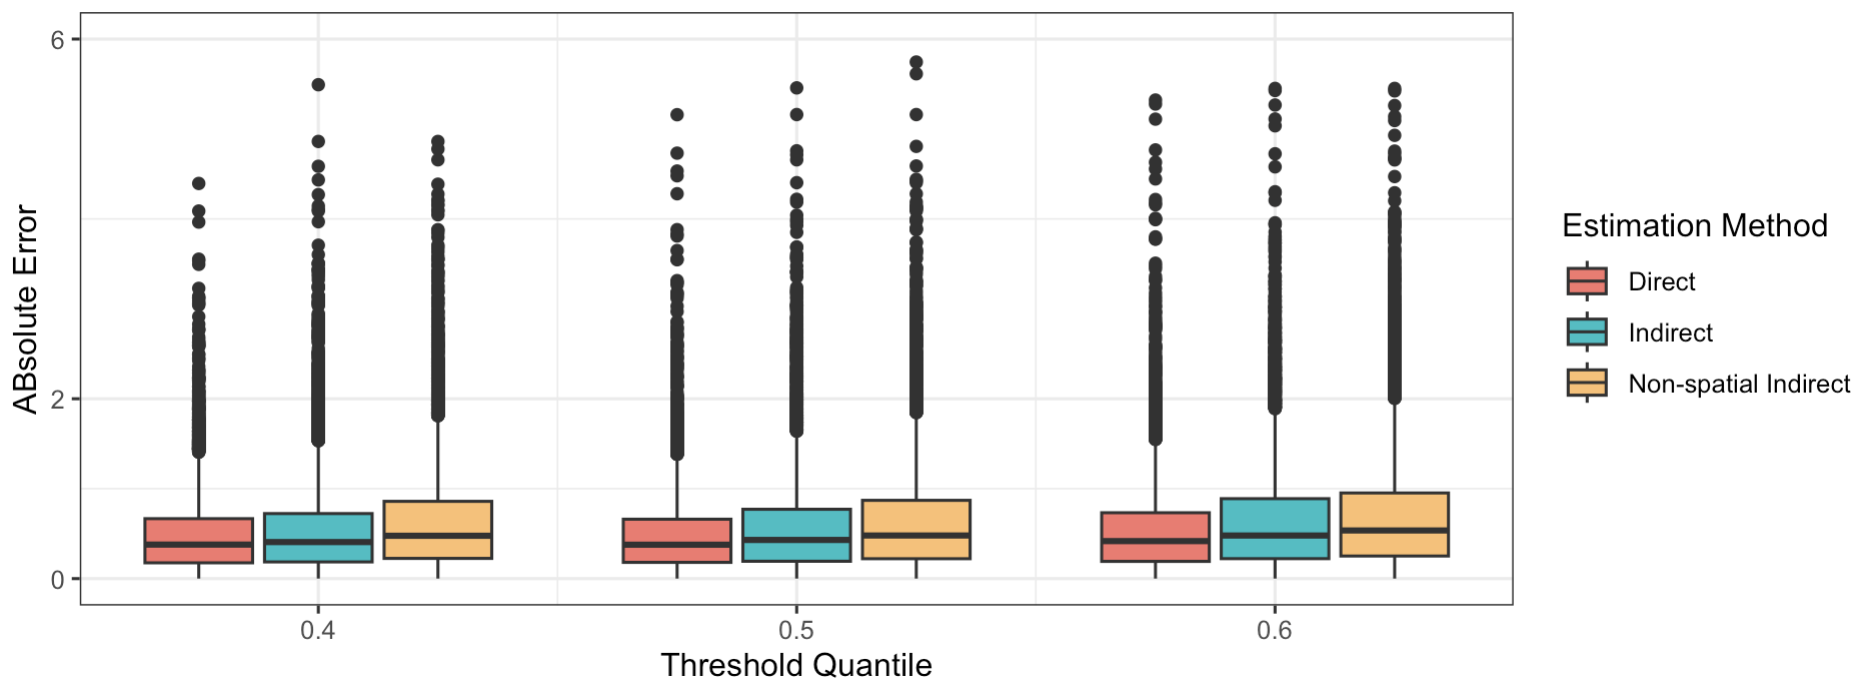
\includegraphics[width=1.00\linewidth]{simulation_boxplot.png}
    \caption{Boxplots of the Absolute Deviation Between the Predicted and True Policies. The x and y-axes show the quantiles of the threshold and the absolute deviation between the predicted and true policies, respectively.}
    \label{fig:sim_boxplot}
\end{figure}

Next, we assess the methods using the following classification performance measures: accuracy, two-sided F1 score, and the Matthews correlation coefficient (MCC). Figure \ref{fig:sim_metrics} shows the results for each method. We also plot the true policy for comparison. The true MRTP performs the best across the different performance measures and all thresholds, validating that the measures are meaningful for evaluating the performance of the policies. Among the estimated policies, the approach accounting for spatial confounding performs better across all thresholds $\mathcal{T}$ and the three performance measures. However, in contrast to the estimation deviation where the direct method outperforms the indirect method (see Figure \ref{fig:sim_boxplot}), the performance of these two approaches is similar across the three measures. This suggests that the estimation advantages of the direct method may not necessarily be reflected in binary classification measures.

\begin{figure}
    \centering
    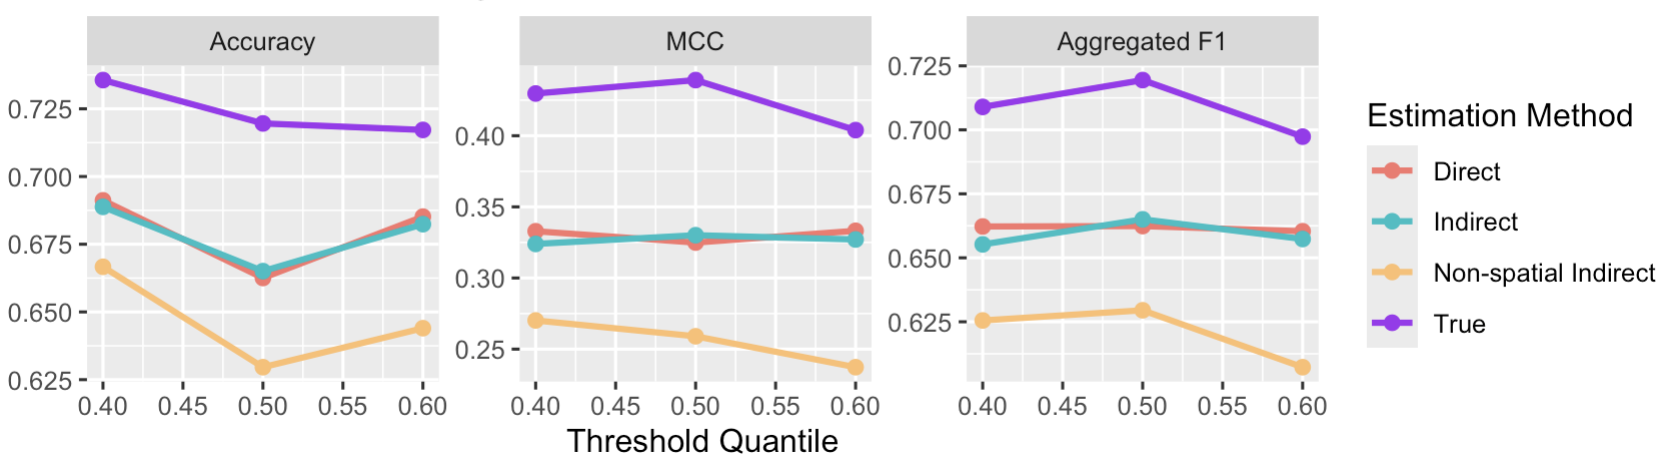
\includegraphics[width=1.05\linewidth]{simulation_metrics.png}
    \caption{Evaluation of Estimated Policy Using Different Measures of Classification Performance. The x-axis shows the threshold. The y-axis shows the value of the measure specified at the top of each plot. A larger value in the y-axis implies better performance.}
    \label{fig:sim_metrics}
\end{figure}
\section{Application: nitrate policy in Wisconsin}\label{sec:application}

\subsection{Background}

Nitrate is the most widespread groundwater contaminant in Wisconsin \citep{saffigna1977nitrate,schubert1999public,mathewson2020health}, affecting both public and private water wells. 
% Excess nitrate of drinking water increases the risk of certain cancers and impacts fetal development during pregnancy \citep{Ward2005, USEPA1995a}.
To protect against health risks imposed by nitrate contaminants, the U.S. Environmental Protection Agency established the drinking water standard for nitrate at 10 mg/L. Exceedance of 5 mg/L nitrate is another critical threshold. Concentrations above 5 mg/L trigger increased monitoring requirements and a health effects statement for public water supply systems. The 5 mg/L threshold is a signal to begin source water protection planning; waiting until 10 mg/L is exceeded is too late. Between 2020 and 2024, approximately 6\% of nitrate measurements in Wisconsin exceeded the 10 mg/L threshold, and 20\% exceeded the 5 mg/L threshold. The exceedance rates are spatially heterogeneous, with some counties showing significantly higher rates (see Figure \ref{fig:exceedance_rate}). 
To obtain a safe water supply, any public water system that has nitrate levels above 10 mg/L is considered in violation and must either replace the well or install approved treatment according to regulation \citep{CFR2016}. For private water systems, well owners of nitrate-contaminated private wells can qualify for the new American Rescue Plan Act (ARPA) Well Compensation and Well Abandonment Grant Program \citep{WIDNR_ARPA_2022} if the nitrate level in their well exceeds 10 mg/L. The cost of well replacement is mainly determined by the depth of the wells drilled. Since October 2022, more than 10 million dollars has been allocated to replace private wells, and more than 40 million dollars has been allocated to replace private wells in Wisconsin. Due to the large number of wells in Wisconsin, the estimated cost to replace all non-compliant wells is over 420 million dollars. In this section, we use our method to design a safe, cost-effective nitrate policy given $\mathcal{T}=$ 5 mg/L in Wisconsin. The policy against $\mathcal{T}=$ 10 mg/L is postponed to the Supplementary Material.

\begin{figure}
    \centering
    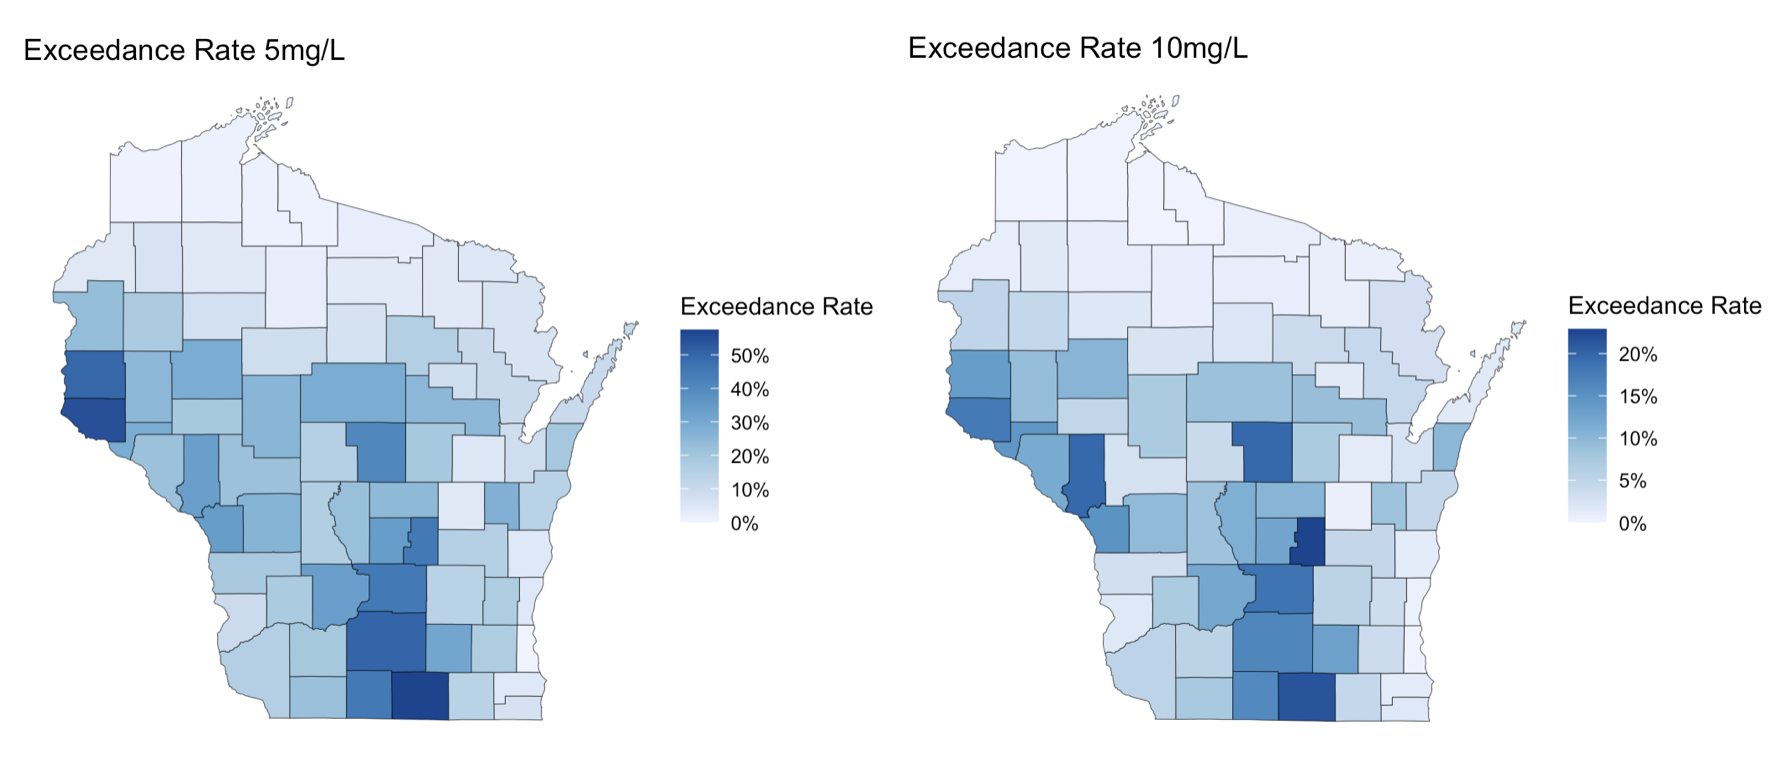
\includegraphics[width=1.05\linewidth]{execeedance rate.png}
    \caption{Exceedance rates of nitrate measurements in Wisconsin counties from 2014 to 2024. Left panel shows the exceedance rate above 5 mg/L. Right panel shows the exceedance rate above 10 mg/L.}
\label{fig:exceedance_rate}
\end{figure}

\subsection{Dataset}

\begin{figure}[htbp]
    \centering
    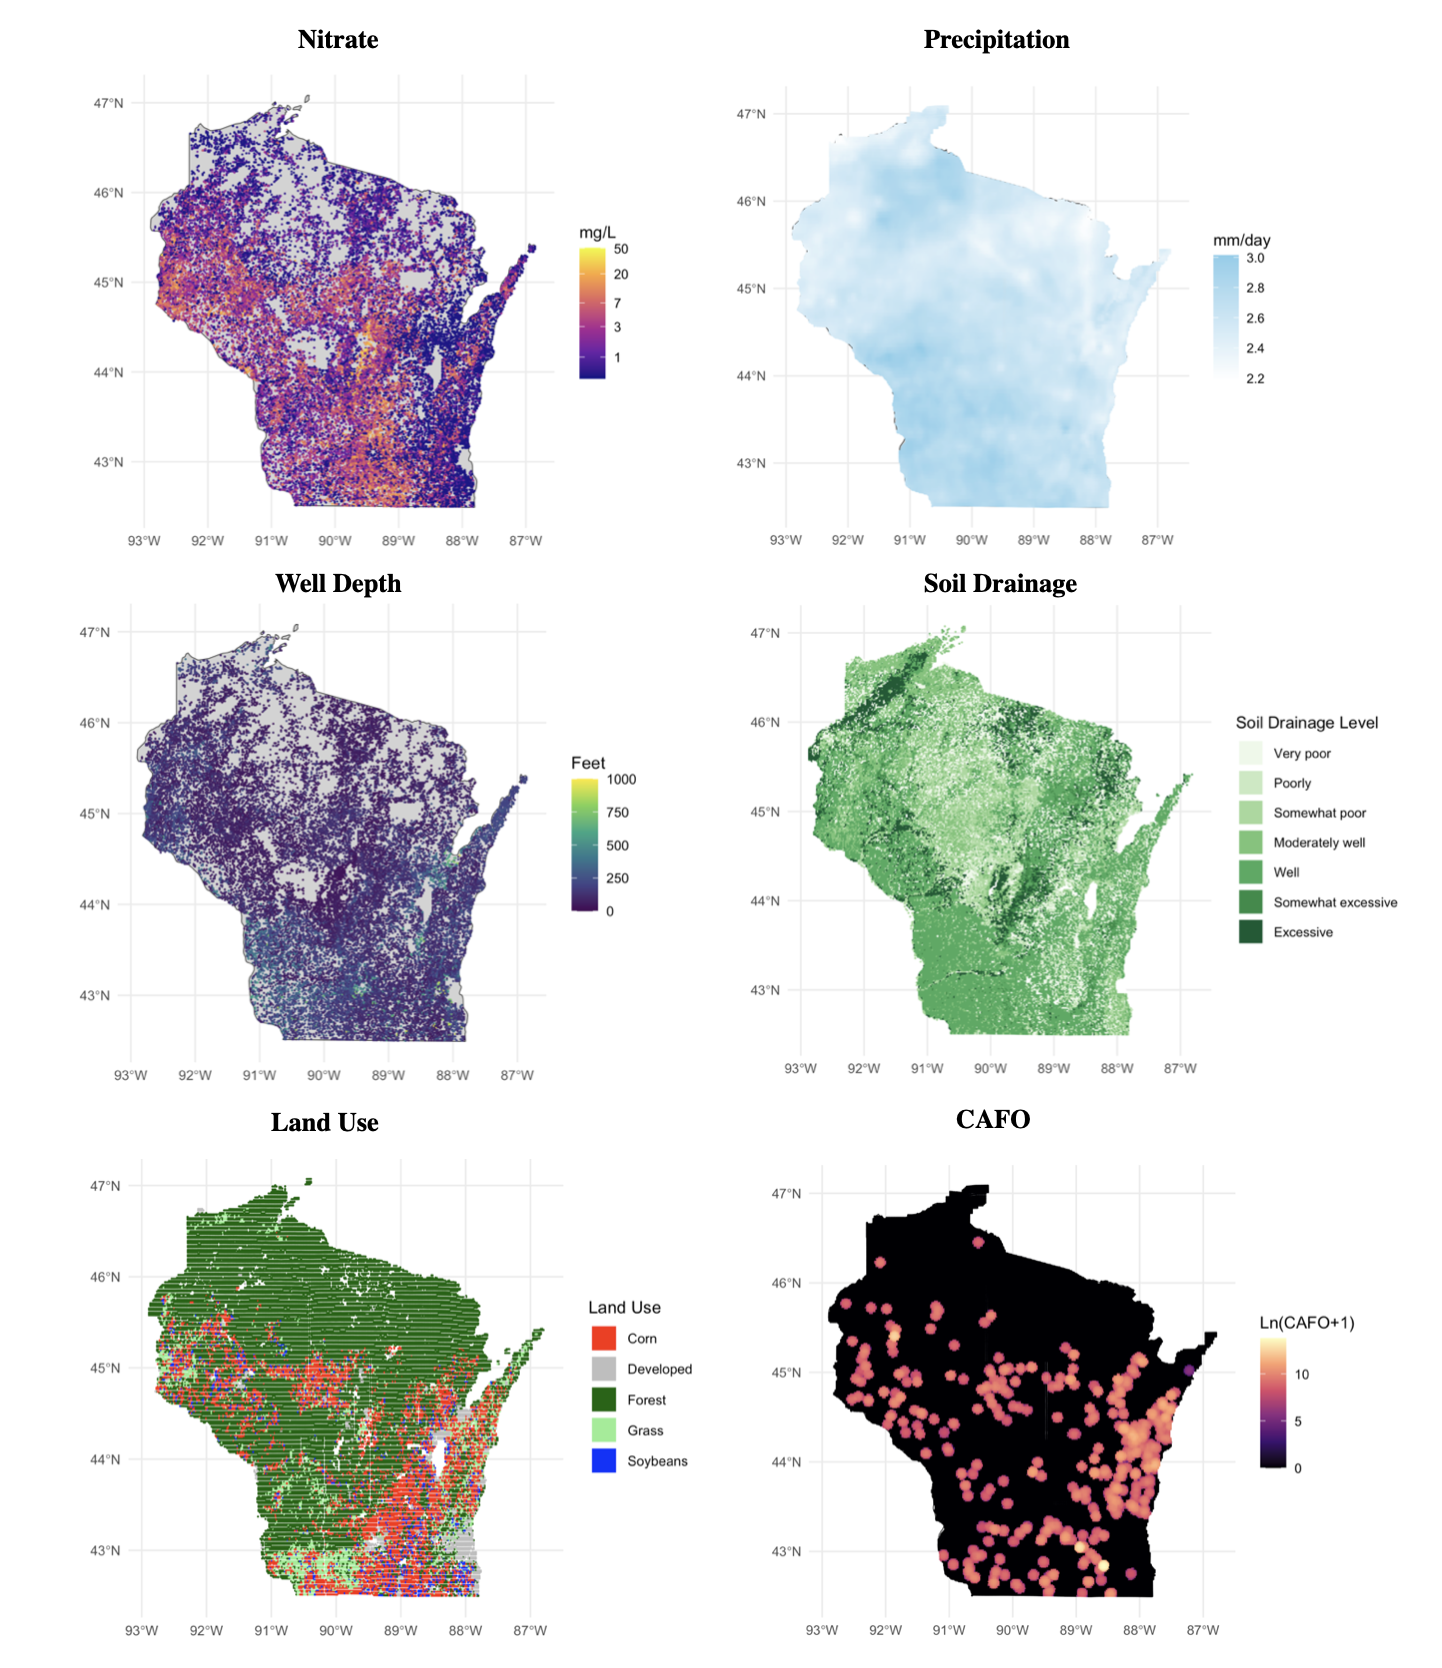
\includegraphics[width=1.00\linewidth]{data_visualization.png}
    \caption{Maps of the dataset displaying nitrate levels, well depth, nitrate sources, and hydrogeological features in Wisconsin.}
\label{fig:nitrate_visualization}
\end{figure}

Groundwater nitrate levels have remained relatively stable over time in both private and public wells. Consequently, we define the observed outcome, $Y_i$, as the log-transformed nitrate measurement obtained between 2020 and 2024. Thus, we let the log-transformed nitrate levels obtained between 2020 and 2024 be $Y_i$, and the corresponding well depth be $A_i$. The primary contributors to groundwater nitrate are agricultural activities, specifically the application of synthetic fertilizers and manure from concentrated animal feeding operations (CAFOs) \citep{Nolan2002, Hudak2000, Spalding1993, Sobota2013, Sabo2018}. Following application, nitrate dissolves in water and percolates through the soil and bedrock into the underlying aquifer. Motivated by this transport mechanism, we specify the predictor vector $X_i$ to include both nitrate sources (land use, CAFOs) and the hydrogeological features affecting transport (soil drainage, precipitation, and static water level). Figure \ref{fig:nitrate_visualization} shows maps of the dataset. See Supplementary Materials for more details on the dataset.



\subsection{Results}


\textbf{Finding 1: The relationship between policy and geographical features}


\noindent The right panel of Figure \ref{fig:policy_and_covariates} illustrates the estimation of a safe, cost-effective nitrate policy relative to a 5 mg/L threshold. Visually, the required minimum well depths are greater in locations with Concentrated Animal Feeding Operations (CAFOs) and intensive agricultural activity. We statistically verified this by projecting the estimated policy onto spatial predictors; the required well depth is positively associated with the CAFO variable ($p\text{-value} \le 2e^{-16}$), and all agricultural land uses exhibit a larger marginal effect relative to the baseline of ``Forest'' (Figure \ref{fig:policy_and_covariates}, bottom-left). These findings align with the understanding that synthetic fertilizers and manure from CAFOs are primary contributors of nitrogen (N), which oxidizes into nitrate in the soil. 

More specifically, among different crop types, we find that the marginal mean of the required well depth is largest for vegetables, followed by corn, and finally soybeans. The high requirement for vegetables is likely driven by potatoes, a dominant crop in Wisconsin. Potatoes possess shallow root systems and low nitrogen use efficiency, often necessitating higher fertilizer application rates than corn to ensure uptake. While corn is also a nutrient-intensive crop, its deeper root system allows for slightly more efficient capture of inputs compared to potatoes. In contrast, soybeans require the lowest level of intervention; as legumes, they maintain a symbiotic relationship with bacteria that fix atmospheric nitrogen, minimizing the need for external fertilizers.

Additionally, the required well depth is significantly influenced by soil drainage and precipitation. As shown in the top-left panel of Figure \ref{fig:policy_and_covariates}, with the exception of the extreme categories (very poorly and excessively drained), the required well depth increases monotonically with soil drainage levels. We also find that precipitation has a positive linear effect ($p\text{-value} \le 2e^{-16}$), indicating that areas with higher rainfall require deeper wells to access safe water. This relationship is driven by the role of precipitation as the primary transport mechanism for nitrate; higher rainfall and drained soil effectively mobilize surface nitrates and drive the contaminant deeper into the aquifer.

\begin{figure}[hbtp]
    \centering
    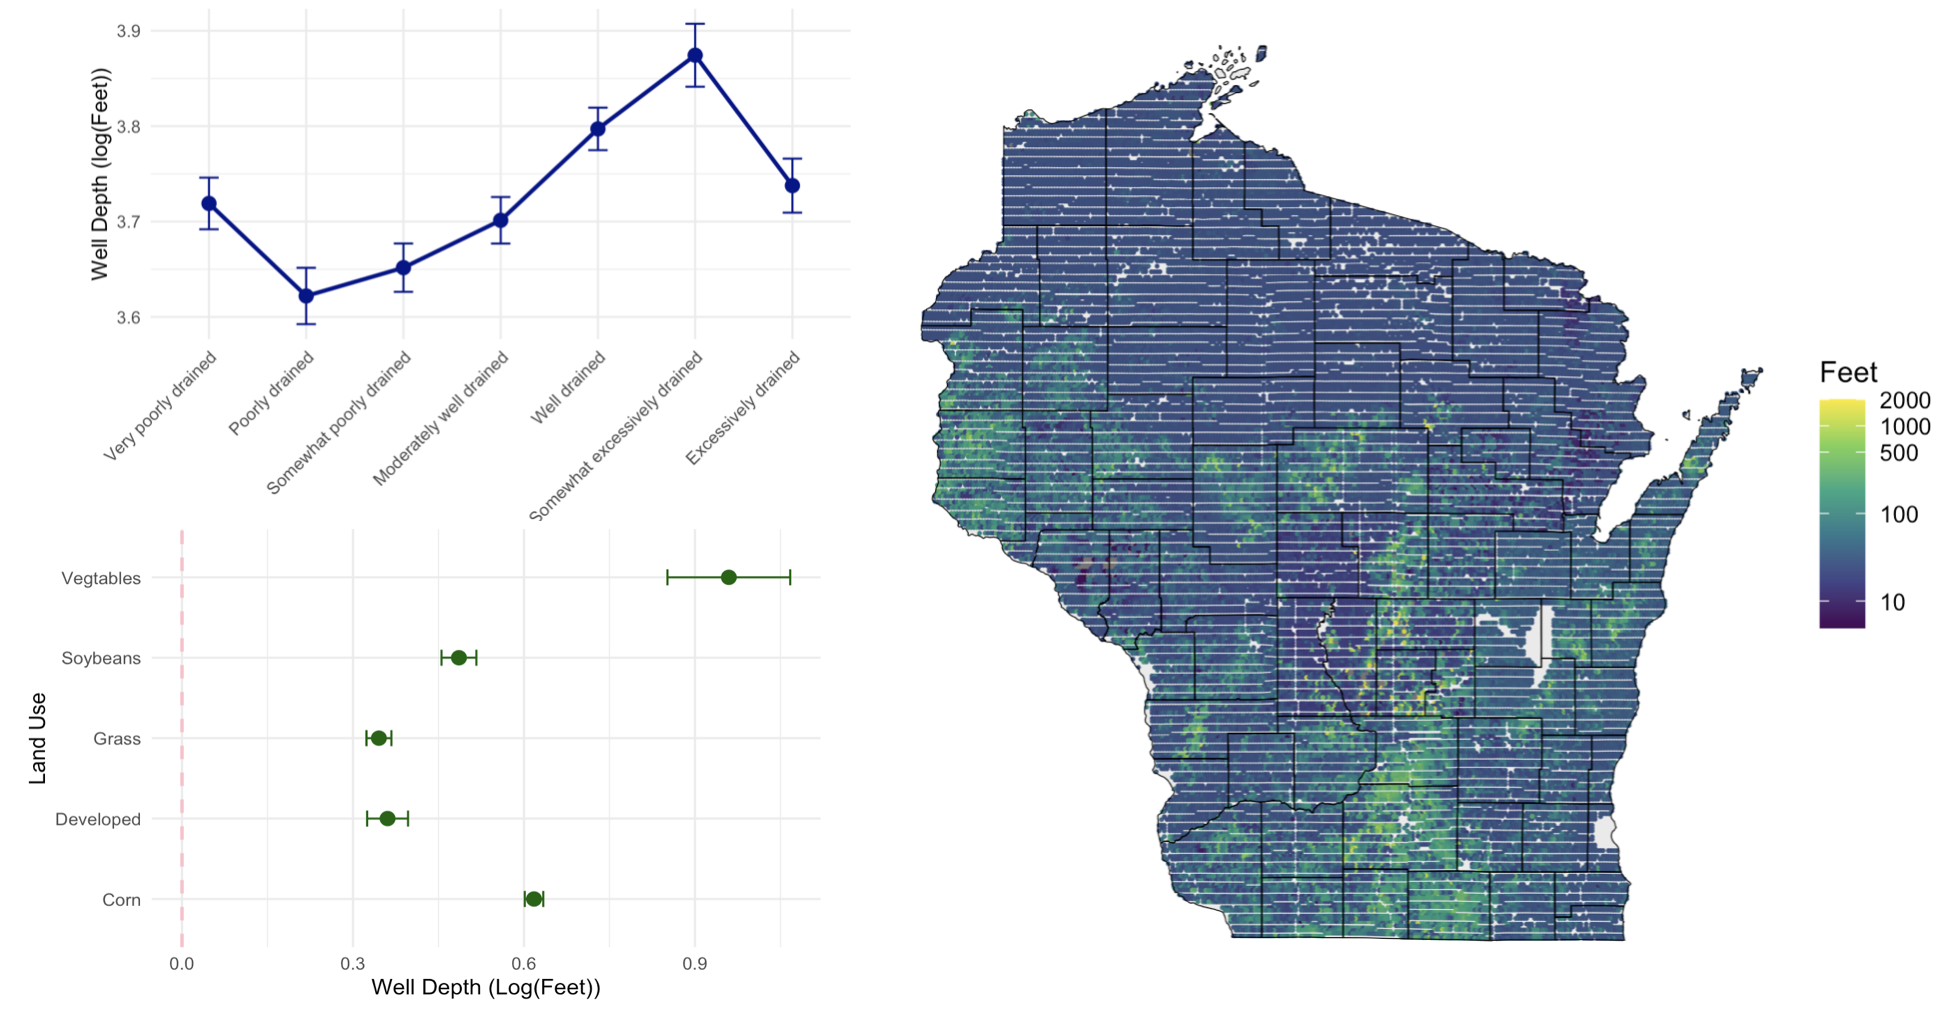
\includegraphics[width=1.0\linewidth]{policy_inference.png}
    \caption{Estimated minimum well depth required to maintain nitrate levels below 5 mg/L using our method. Left: Marginal effects of drainage level (top) and land use (bottom). Right: Spatial distribution of the required well depth.}
    \label{fig:policy_and_covariates}
\end{figure}

\noindent\textbf{Finding 2: Comparison between our method and non-spatial method}

To show the importance of accounting for spatial confounding and dependence in environmental observational studies, we compared the performance of our proposed method against the indirect method that relies on assumptions of unconfoundedness and i.i.d. observations in the nitrate dataset. We randomly partitioned the nitrate dataset into training (70\%) and test (30\%) sets, using the training data to estimate the policy. Table \ref{tab:model_performance} shows the classification performance metrics. Across all measures, our approach consistently outperforms the non-spatial indirect method. 

Figure \ref{fig:indirect_inference} depicts the projection of the policy estimated via the non-spatial method onto spatial predictors. The left panel shows the marginal effects of various land use categories. While the non-spatial method correctly identifies the general increase in required well depth associated with agricultural activities, it lacks the resolution to distinguish between specific crop types. Specifically, the confidence intervals for corn and soybeans overlap and are nearly indistinguishable from those of vegetables (potatoes). In the right panel, which displays the marginal effects of soil drainage, the monotonic trend observed in our proposed method is obscured and exhibits considerably less stability. We attribute these inconsistencies to the violation of the unconfoundedness assumption, where the effects of unmeasured spatial confounders are misattributed to the observed predictors. In contrast, our method, which incorporates spatial confounding, mitigates this bias and yields more reliable estimates of the effects of geographical features.

\begin{figure}[htbp]
    \centering
    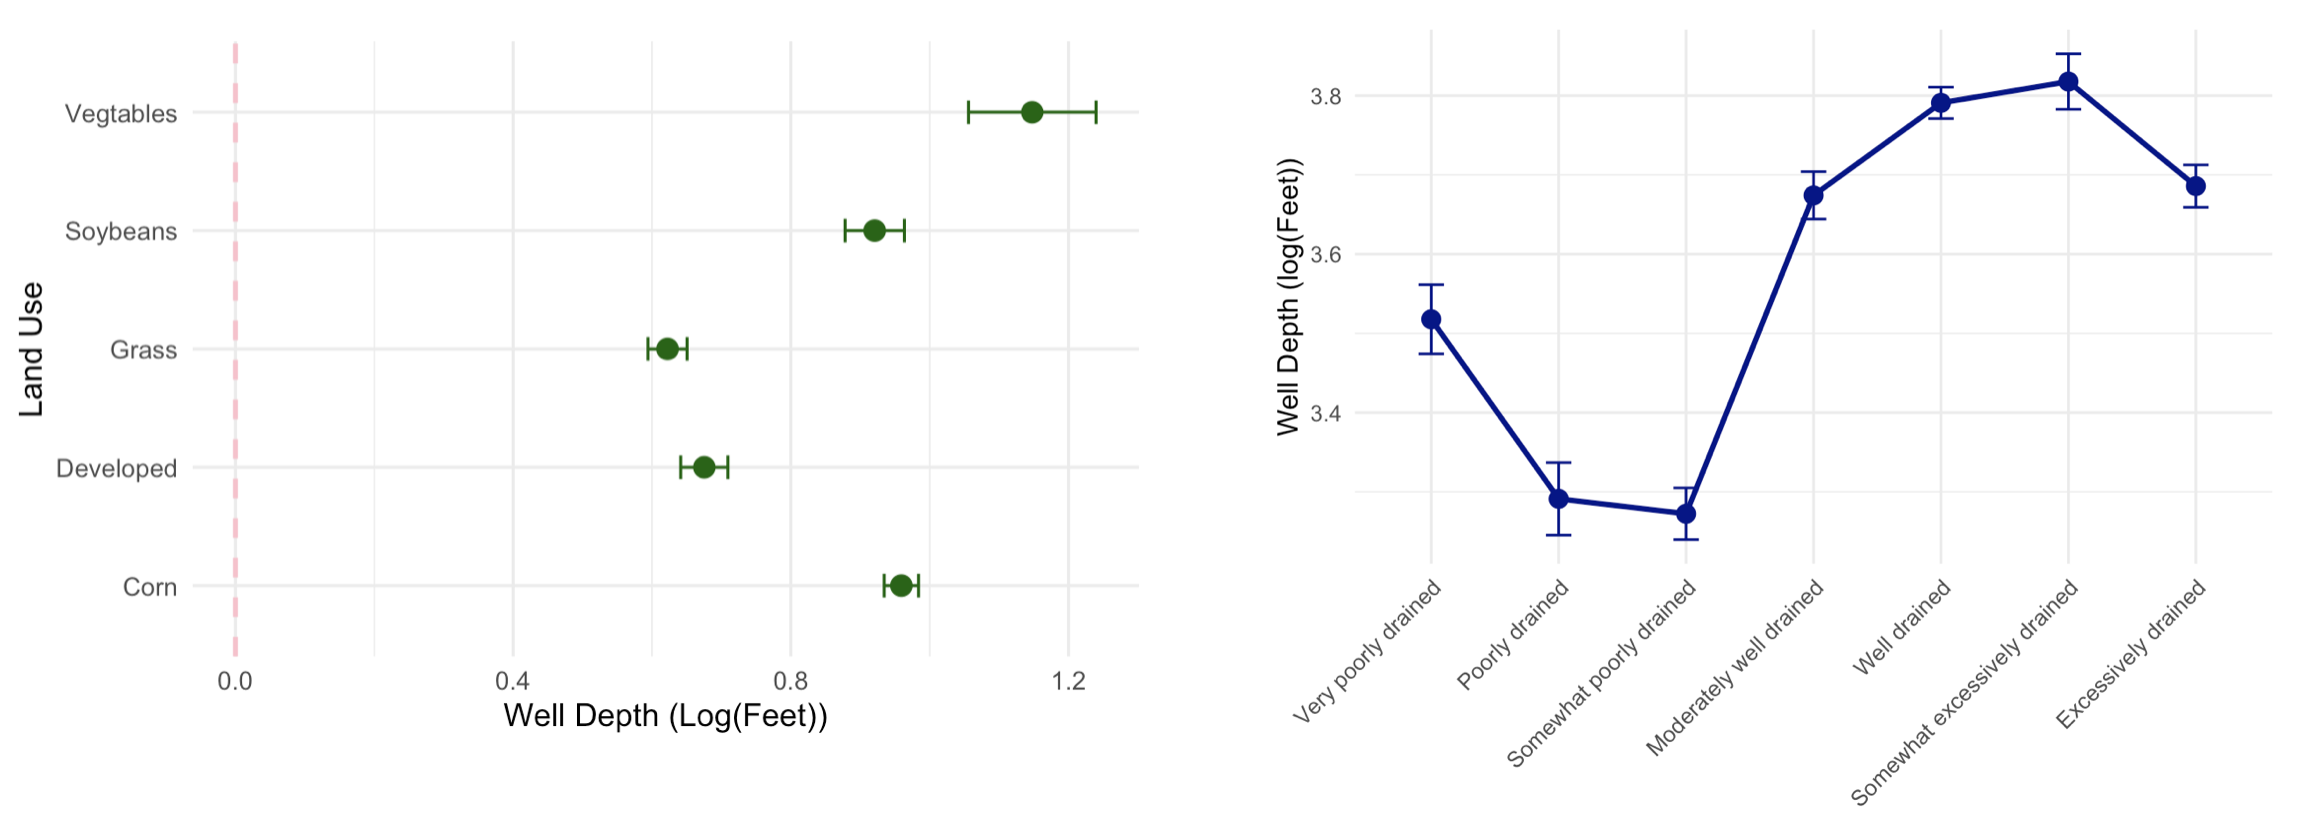
\includegraphics[width=1.05\linewidth]{indirect_inference.png}
    \caption{Marginal effects on the minimum well depth required estimated by the non-spatial method to maintain nitrate levels below 5 mg/L. The left panel shows the effect of land use categories. The right panel shows the effects of drainage level.}
    \label{fig:indirect_inference}
\end{figure}

\begin{table}[htbp]
    \centering
    \caption{Evaluation of nitrate mitigation policy estimated by the non-spatial indirect method and our method using binary classification measures.}
    \label{tab:model_performance}
    \begin{tabular}{l cc cc}
        \toprule
        & \multicolumn{2}{c}{\textbf{Training Data}} & \multicolumn{2}{c}{\textbf{Test Data}} \\
        \cmidrule(lr){2-3} \cmidrule(lr){4-5}
        \textbf{Metric} & Non-spatial & Our Method & Non-spatial & Our Method \\
        \midrule
        Two-sided F1 & 0.669 & \textbf{0.790} & 0.664 & \textbf{0.759} \\
        MCC          & 0.401 & \textbf{0.590} & 0.388 & \textbf{0.531} \\
        Accuracy     & 0.767 & \textbf{0.833} & 0.763 & \textbf{0.810} \\
        \bottomrule
    \end{tabular}
    
    \vspace{0.2cm}
    \footnotesize{\textit{
    Note: Higher values of all three metrics indicate better performance.
    }}
\end{table}
\section{Discussion}
In this paper, motivated by the groundwater nitrate contaminants and the required mitigation intervention, we develop a statistical framework for learning safe, cost-effective policies for continuous treatments in the presence of unique challenges posed by environmental observational data, the spatial confounding and dependence. We established identification conditions that use spatial location as a proxy for unmeasured confounders. Then we propose two methods for estimating the safe, effective policies, an indirect method utilizing geospatial machine learning, and a direct method where a nonparametric, doubly robust loss function is used inside of an empirical risk minimization problem. We derive excess risk bounds of our method accounting for the spatial dependence and the use of kernel smoothing. We then use the direct method to estimate a safe, cost-effective policy for nitrate mitigation in Wisconsin by using the nitrate measurements from 2014 to 2024. Compared to the method method that does not account for the spatial confounding, we show that our method is more accurate and can recover scientifically interpretable relationships.

We conclude by discussing the potential future directions of our work. First, from the modeling perspective, our framework imposes three key assumptions: (i) the spatial confounder is additively separable from the measured covariates (a constraint of the spatial mixed effects model); (ii) the policy’s dependence on covariates is restricted by the kernel SVM specification, and (iii) the nuisance functions belong to VC-type classes. An interesting future direction would be to relax these constraints by integrating modern AI and machine learning architectures to further improve the flexibility. Second, from the computational perspective, although our framework integrates numerical approximations for Gaussian processes, the empirical minimization of the proposed risk functions remains challenging for continuous treatments due to the lack of a closed-form solution. A promising avenue for future research is to adapt scalable Bayesian computation techniques to the problem of spatial policy learning.

\bibliography{ref}


% \textcolor{red}{Check the minimum depth at forest, it should be forest. This can actually be integrated in loss function where we use location specific range.}

% \textcolor{red}{Depth map of several region based on two threshold. The scatter plot of nitrate level v.s. covariate. The scatter plot of minimum depth v.s. covariate. Map of covariate.}


% \textcolor{red}{Contrast with policy does not take into account spatial confounding, current depth map, map of kriging estimation of U.}








\clearpage
\section*{Supplementary Material}

\appendix


This document contains supplementary materials for ``Optimal Policy Learning Spatial Confounding.'' Section \ref{sec:data source} presents details of the nitrate dataset. Section \ref{sec:A} presents computational details related to the main paper. 
Section \ref{sec:B} proves lemmas and theorems stated in the paper.

\section{Details of Data Sources and Preprocessing}\label{sec:data source}

\subsection{Nitrate Measurement}

The Wisconsin Department of Natural Resources (DNR) maintains the Groundwater Retrieval Network (GRN) to record groundwater quality throughout the state of Wisconsin. The Groundwater Retrieval Network (GRN) reports well information and well sample result data from several DNR databases, including the Public Land Survey System (PLSS) database, the Wisconsin well database, and the sample history of specific groundwater pollutants for specific wells.

\subsubsection{Public Land Survey System}\label{sec:plss}

When the land was first surveyed in Wisconsin, it was divided into a grid as shown in Figure \ref{fig:plss}. Each grid cell represents approximately 36 square miles (the measurements were not always precise due to the instruments the surveyors were using, among other limitations). This grid system is known as the Public Land Survey System (PLSS). Each cell in the grid is identified by a \textit{township} and \textit{range} number. The range number identifies how many cells the property is to the east or west of a starting point. Both eastern and western ranges are possible in Wisconsin. The township number identifies how many cells the property is to north or south of a starting point. Only northern townships are possible in Wisconsin. Each 36-square-mile parcel identified by a township and range number is further divided into 36 \textit{sections}, each section theoretically being 1 square mile or 640 acres. Many parcels of land are smaller than an entire section. They sometimes are the size of a quarter section. Each section is divided into 4 \textit{quarters}, each being 1/4 square miles or 160 acres. An example of a legal description using the PLSS is ``S24, T32N, R18E'' where the township number is 32 north, range number is 18 east, and section number is 24, as shown in Figure \ref{fig:plss}.


\begin{figure}
    \centering
    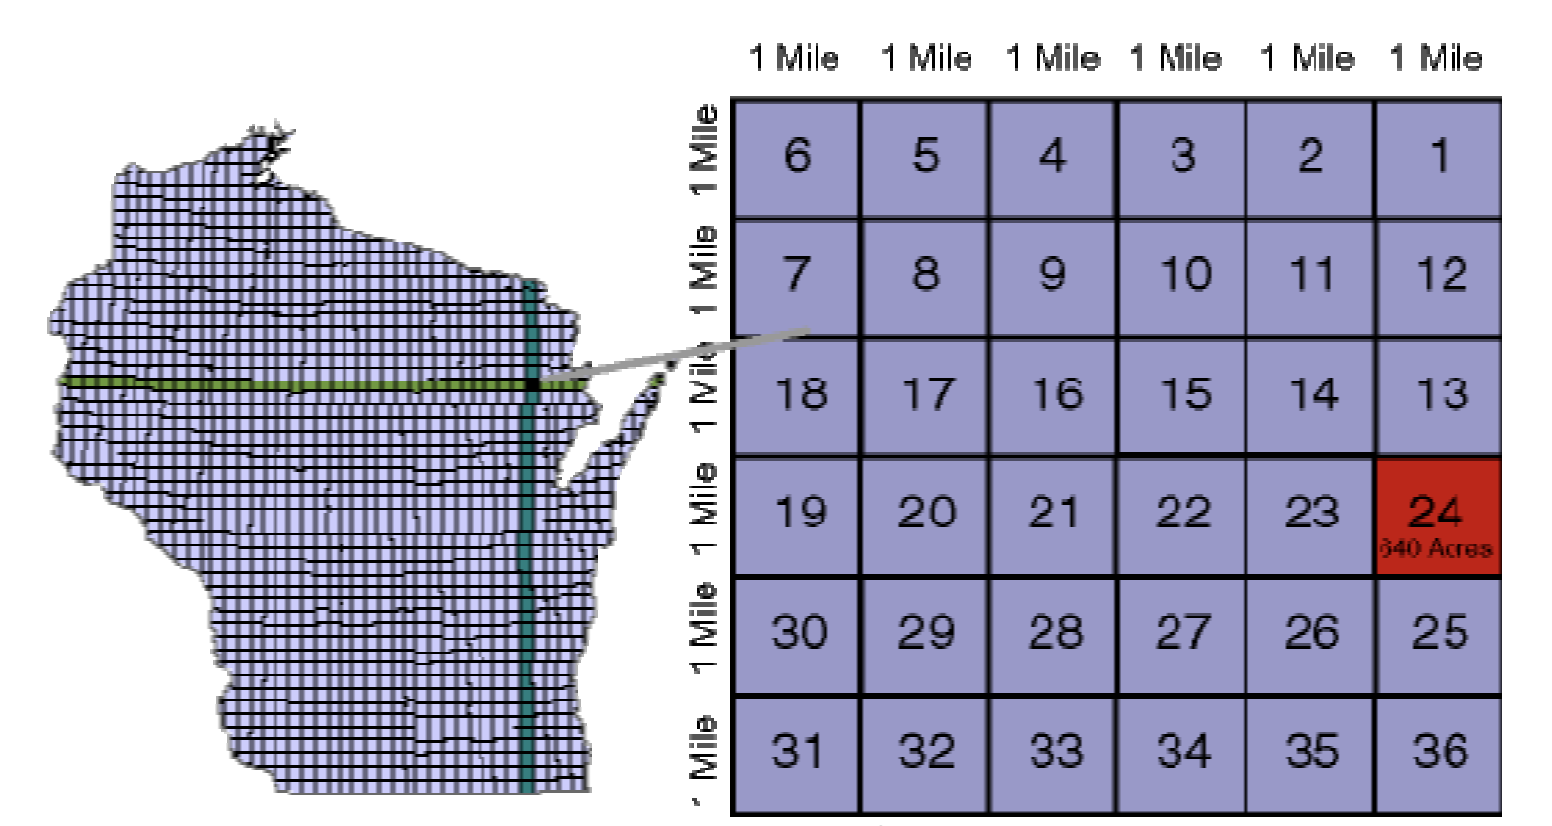
\includegraphics[width=1\linewidth]{plss-example.png}
    \caption{PLSS in Wisconsin}
    \label{fig:plss}
\end{figure}


\subsubsection{Wisconsin Wells}

\textit{Wisconsin Wells} dataset is the well inventory used by the Groundwater Retrieval Network application. Each well has a unique well ID and the locations of wells are recorded using the PLSS descriptions. The dataset has the geographical information of the wells, including the well bottom depth, the casing depth, the bedrock depth, and the static water level. 

As shown in Figure \ref{fig:well}, casing Depth is the depth to which the well casing extends below the ground surface, where the casing serves to stabilize the wellbore and prevent contamination from surface or subsurface sources. The static water level refers to the distance from the ground surface to the water surface in a well when the well is at rest. The well bottom depth indicates where the bottom of the well is located. The Bedrock depth refers to the distance from the ground surface to the top of the bedrock layer. However, in the center part of Wisconsin where bedrock may be near or at the surface, the bedrock depth is invalid. 
\begin{figure}
    \centering
    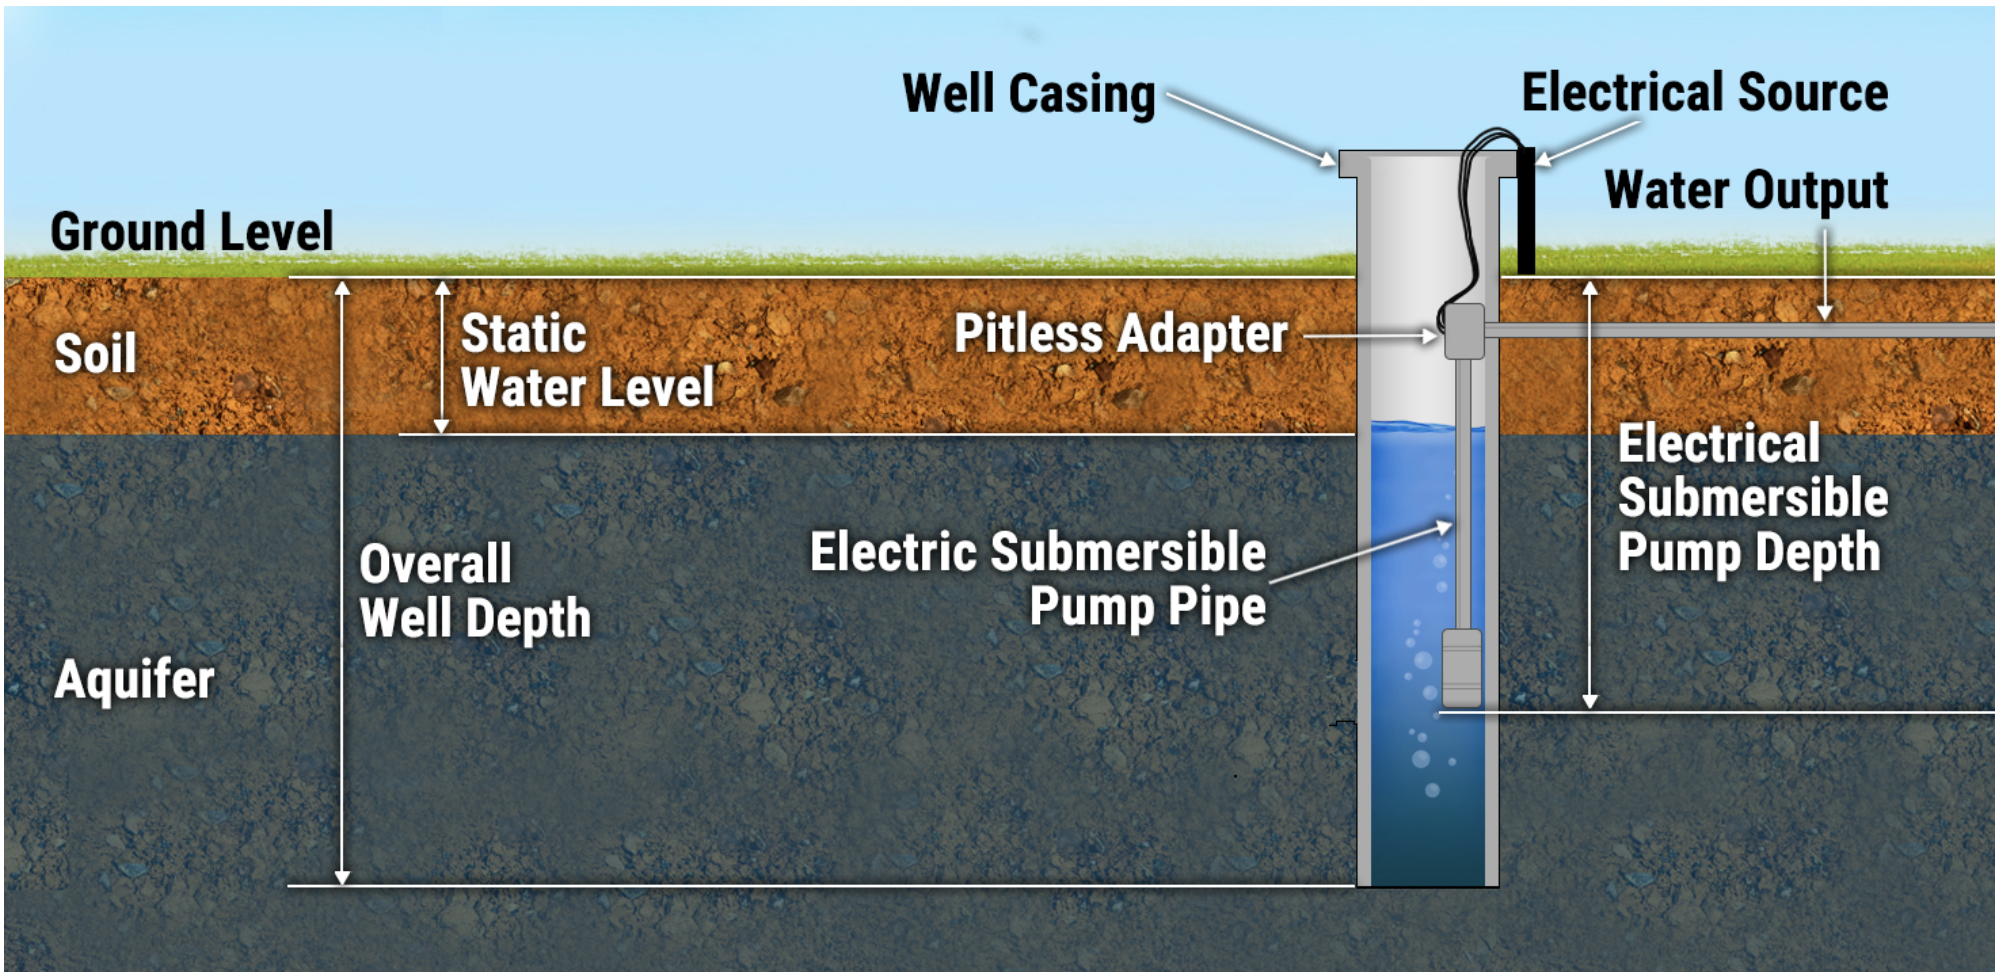
\includegraphics[width=1\linewidth]{well.png}
    \caption{Well geography}
    \label{fig:well}
\end{figure}
The static water level and well depth are the two factors that significantly influence how contaminants interact with and affect well water. Figure \ref{fig:staticlevel} and Figure \ref{fig:welldepth} show the static water level and depth of wells in Wisconsin. The well depth is calculated by
$$\text{Well Depth} = \text{Static Water Level} + \frac{\text{Well Bottom}-\text{Static Water Level}}{2}.$$

\begin{figure}
    \centering
    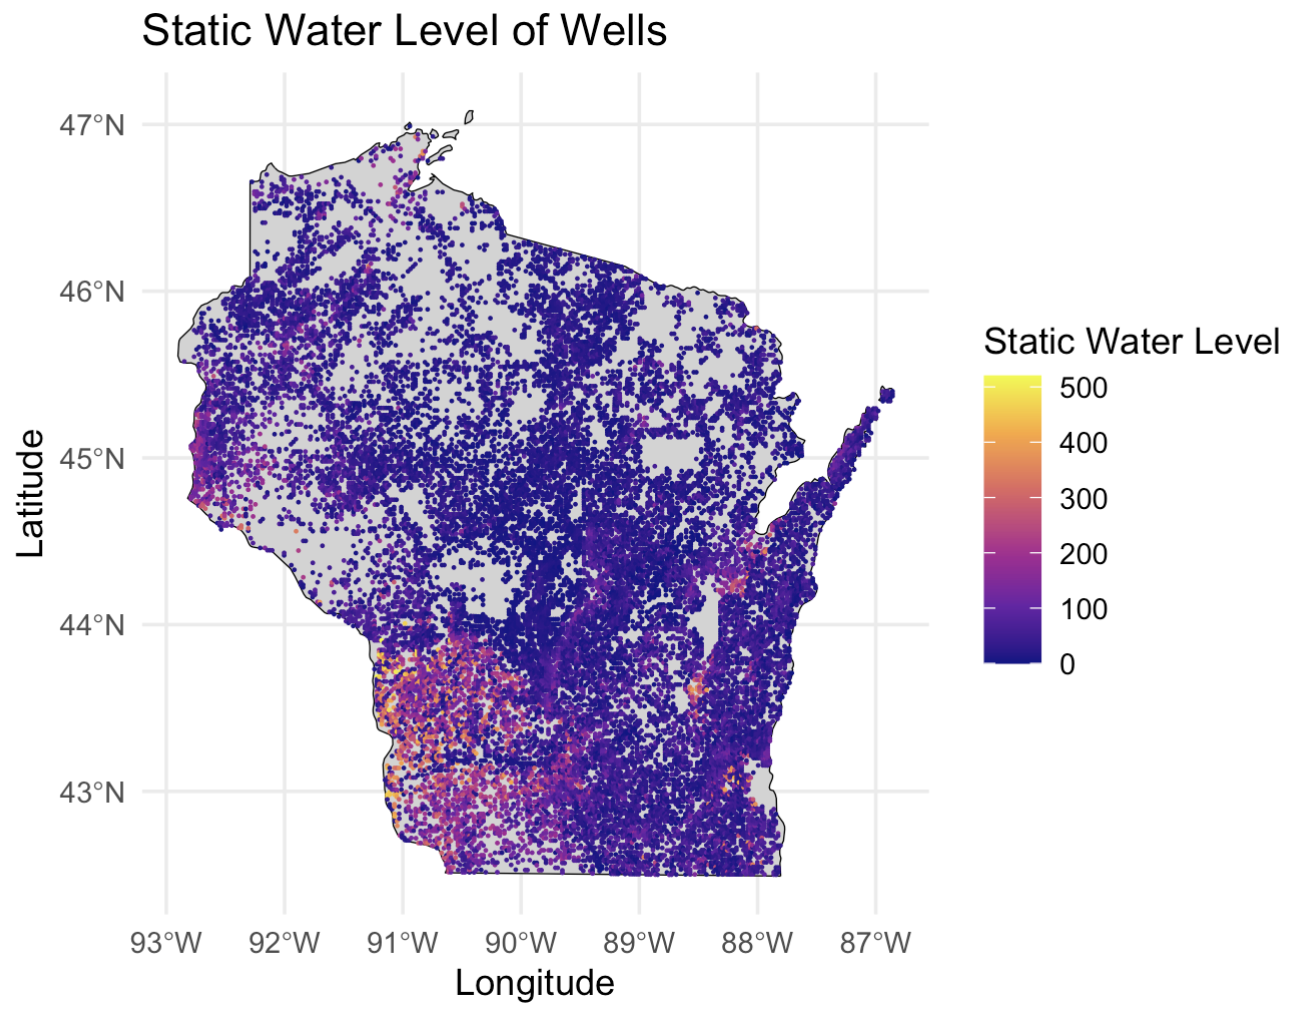
\includegraphics[width=0.7\linewidth]{staticlevel.png}
    \caption{Static water level of wells in Wisconsin}
    \label{fig:staticlevel}
\end{figure}

\begin{figure}
    \centering
    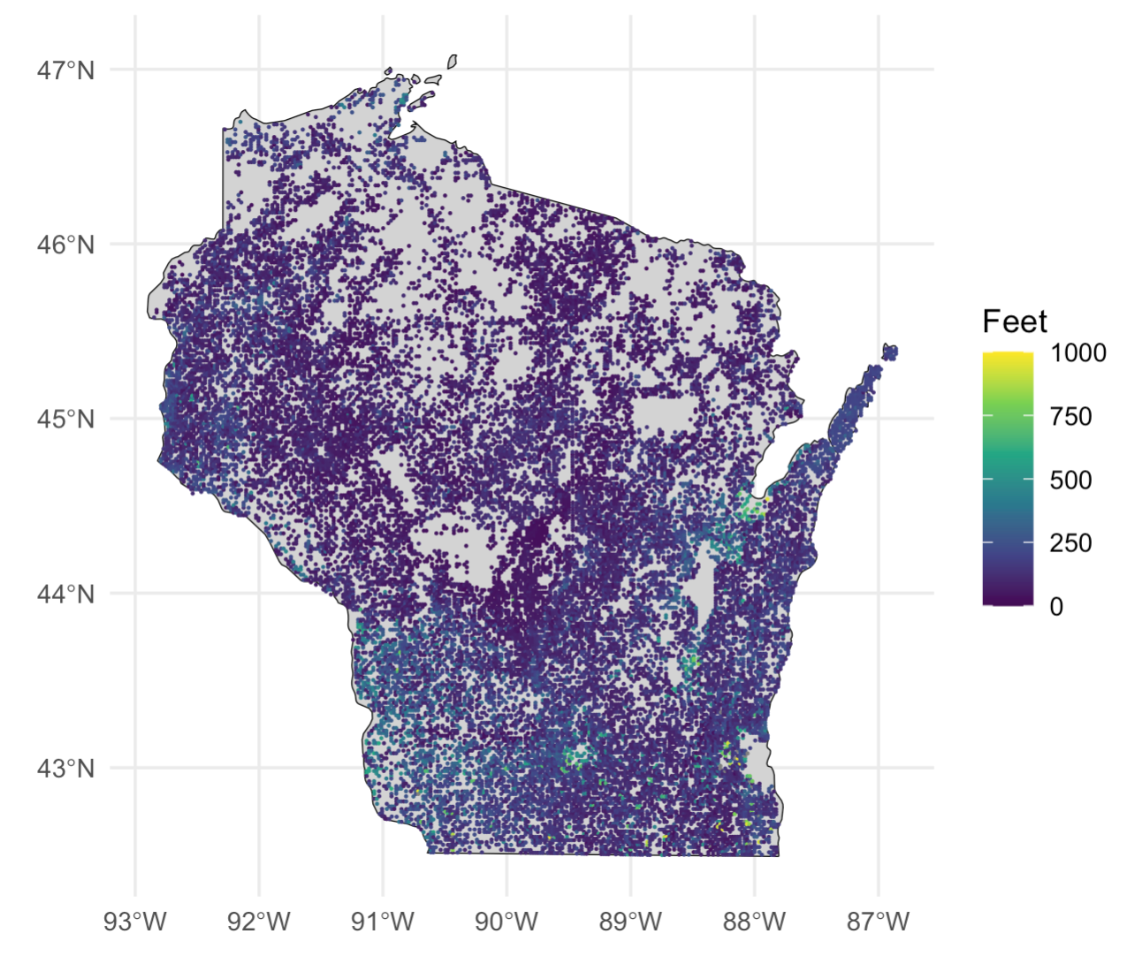
\includegraphics[width=0.7\linewidth]{welldepth.png}
    \caption{Well depth in Wisconsin}
    \label{fig:welldepth}
\end{figure}


% The dataset also records the usage information of wells. For example, private potable well is used for drinking and household use owned by individuals. Private non-potable well is used for non-drinking purposes like lawn irrigation or livestock use. Municipal community wells serve as drinking water for communities. Different types of wells are designed with distinct standards, features, and regulatory requirements, depending on their purpose, usage, and the populations they serve.




\subsubsection{Nitrate}

The Wisconsin Department of Agriculture, Trade and Consumer Protection (DATCP) performs routine monitoring for nitrate. DATCP's Bureau of Laboratory Services (BLS) analyzes samples for nitrate using modern analytical methods. Biased monitor programs are conducted annually. For example, the targeted sampling program and field-edge monitoring program analyze groundwater samples from monitoring wells and private wells installed within or near agriculture fields. The random statewide survey is conducted every 5 or 10 years. Figure \ref{fig:nitrate count} shows the number of measurements (log-scale) that happen at each PLSS section from 2014 to 2024. Figure \ref{fig:nitrate-county} shows the percentage of measurement exceeding 10mg/L nitrate health standard by counties in Wisconsin. 
\begin{figure}
    \centering
    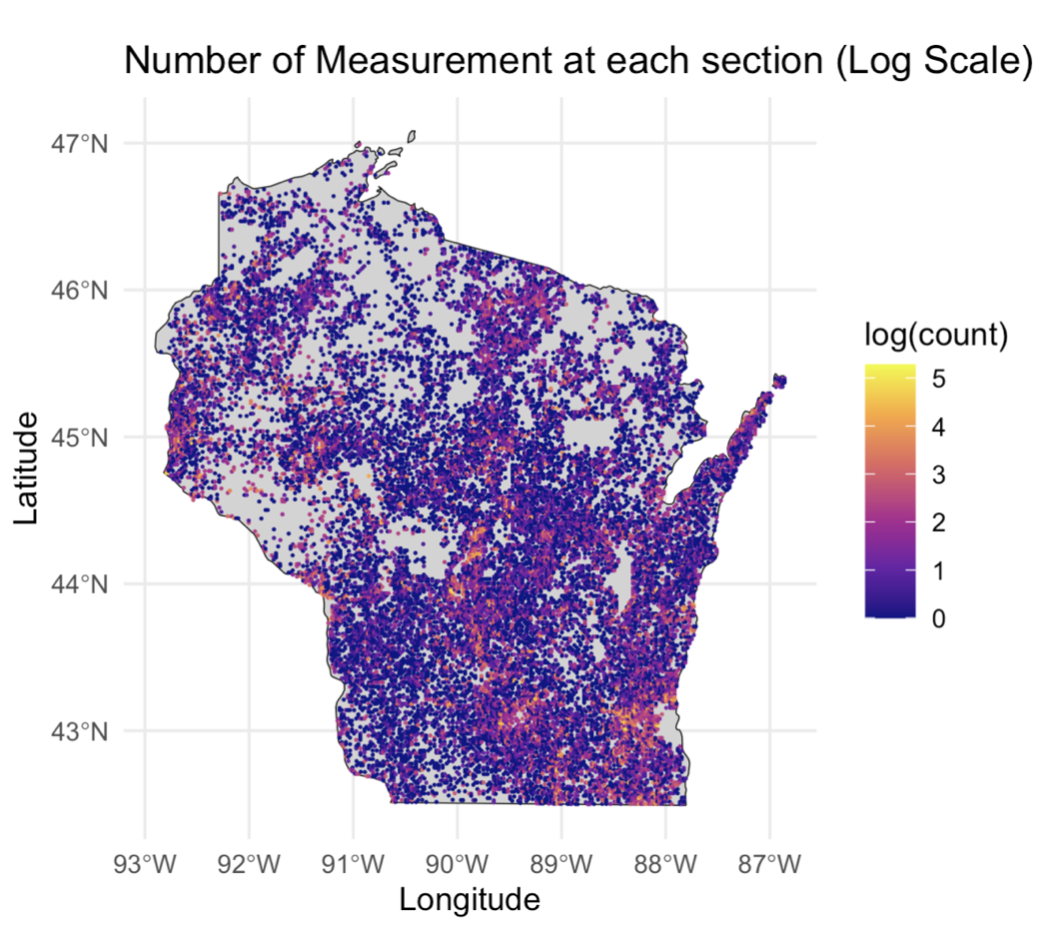
\includegraphics[width=0.65\linewidth]{nitrate-count.png}
    \caption{The average number of measurements of groundwater in Wisconsin}
    \label{fig:nitrate count}
\end{figure}

\begin{figure}
    \centering
    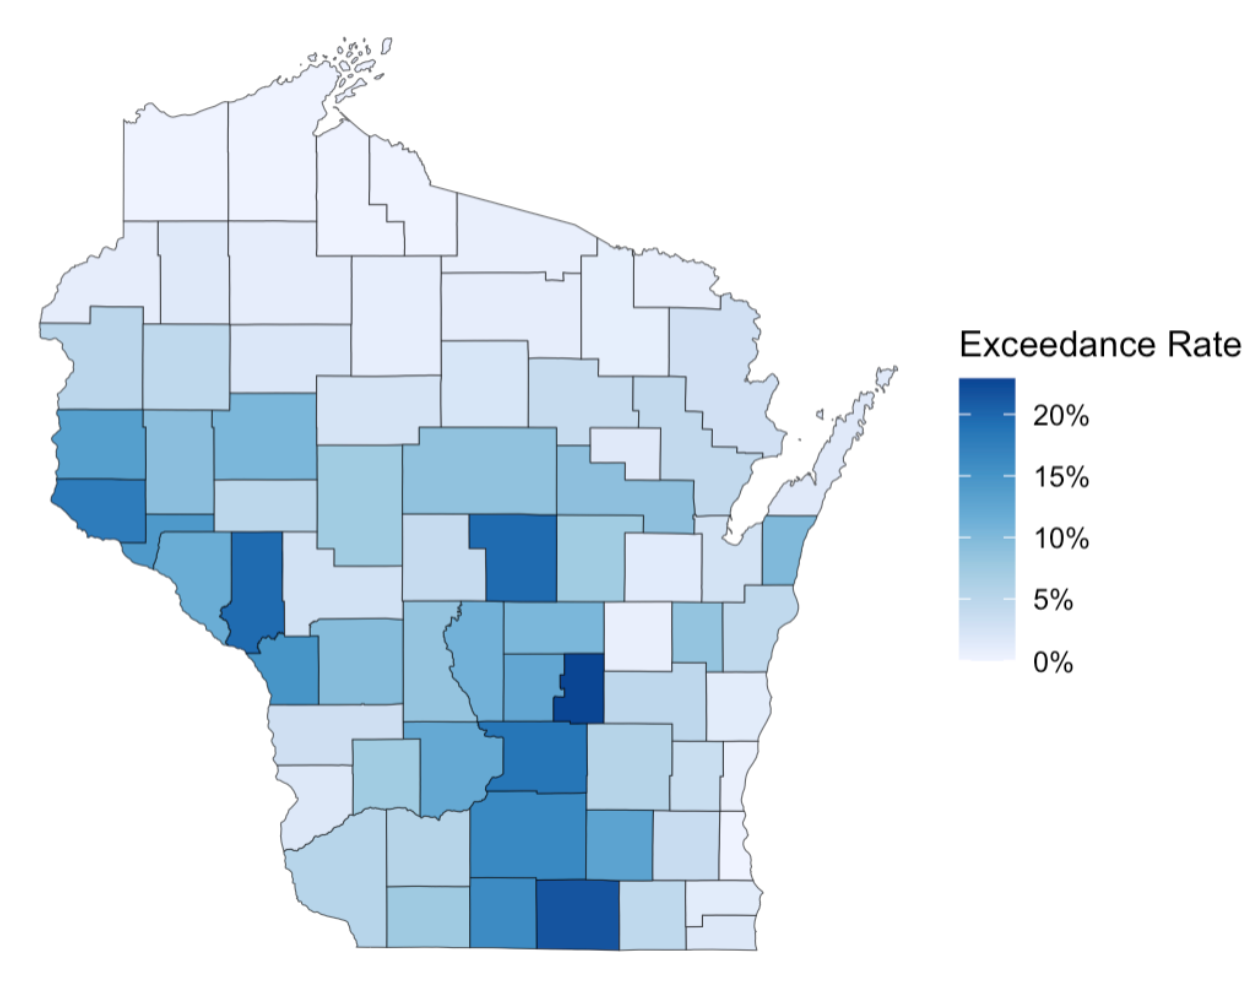
\includegraphics[width=0.6\linewidth]{nitrate-county.png}
    \caption{Percentage of  nitrate measurement over standard (10 mg/L) by county}
    \label{fig:nitrate-county}
\end{figure}

The measurements can be retrieved from the Groundwater Retrieval Network (GRN), which gives the well information, the concentration amount, and the time of the measurement. Figure \ref{fig:nitrate-spatial} shows the nitrate concentration measurement in groundwater from 2014 to 2024. The groundwater in regions with high nitrate concentration is sampled and measured much more frequently (See Figure \ref{fig:nitrate count}).

\begin{figure}
    \centering
    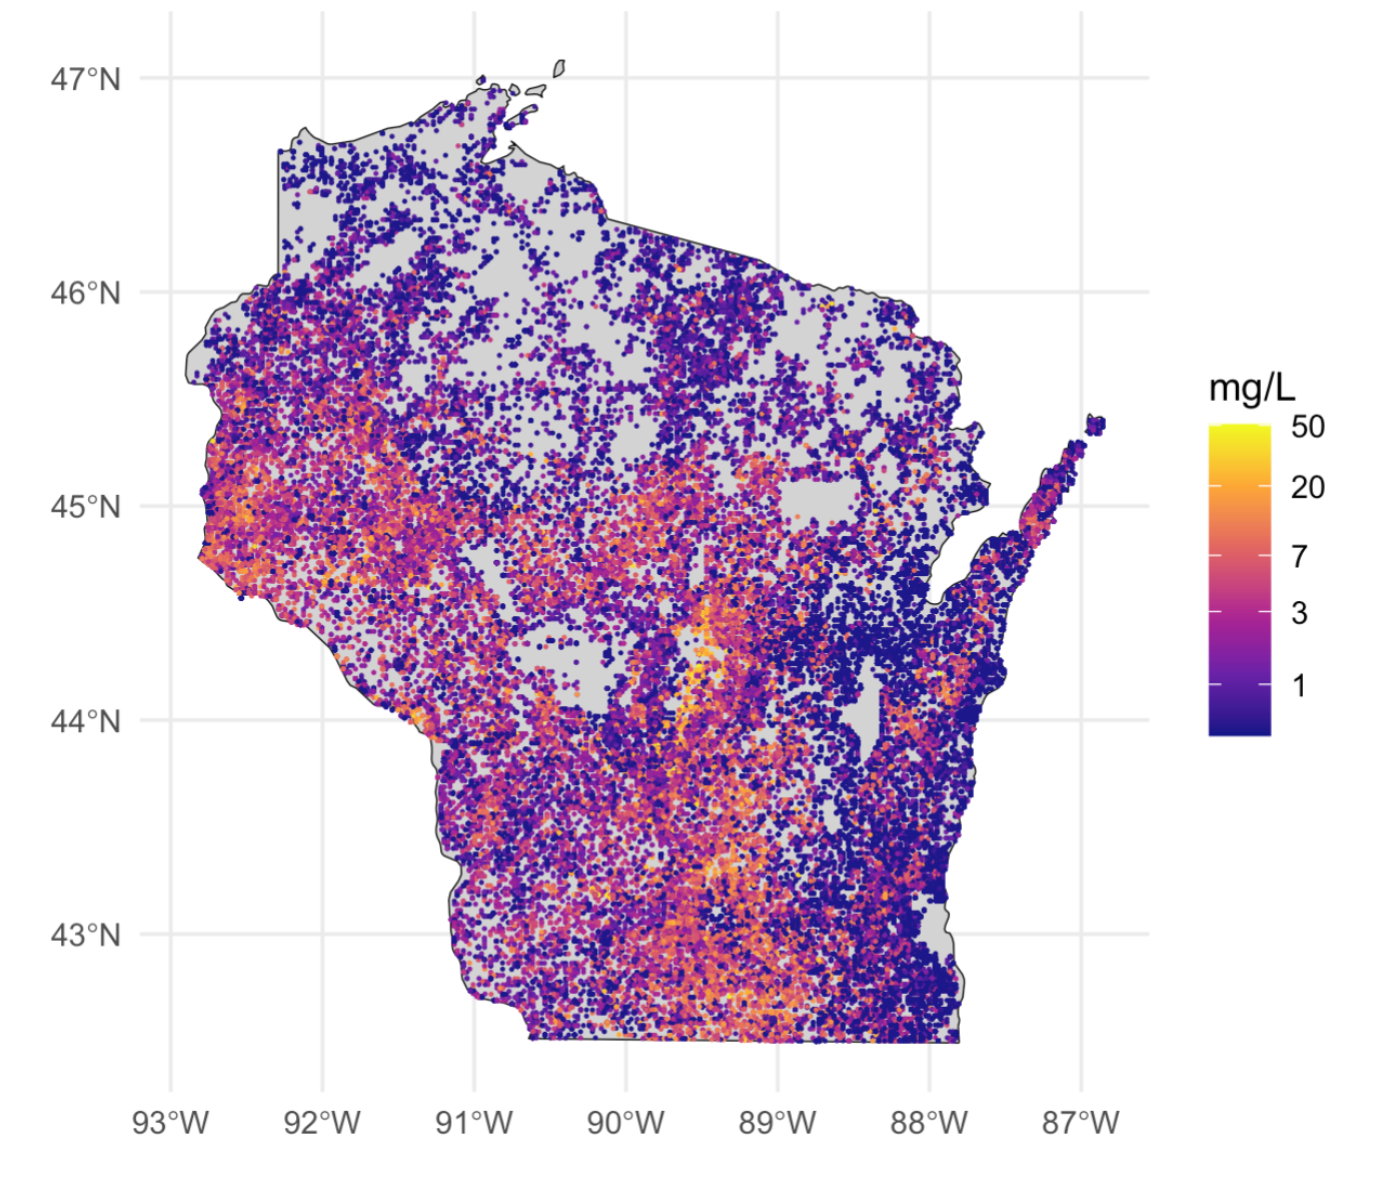
\includegraphics[width=0.6\linewidth]{nitrate-spatial.png}
    \caption{Ground water nitrate concentration in Wisconsin from 2014 to 2024}
    \label{fig:nitrate-spatial}
\end{figure}



\subsection{Spatial Covariates and Preprocessing}

% Nitrate concentrations in groundwater depend on numerous factors such as land use, agricultural fertilizer application practice, hydrological and hydrogeological conditions, soil properties, weather conditions, and livestock manure. 
In this section, we introduce the collection and assign spatial covariates to each PLSS section (See Section \ref{sec:plss} ) in Wisconsin. 



\subsubsection{Land Cover}

The Cropland Data Layer (CDL) is a data product produced by the National Agricultural Statistics Service of U.S. Department of Agriculture. It provides geo-referenced, high accuracy, 30 or 56-meter resolution, crop-specific cropland land cover information for up to 48 contiguous states in the U.S. from 1997 to the present. We use the \texttt{CropScapeR} package to download CDL data of Wisconsin. 

A PLSS section might has different types of land cover. To address this issue, we select the crop type that dominates the PLSS section as its value of the covariate ``Land Cover''. There are 69 different land cover categories in Wisconsin in total. We combine them into nine different land cover categories based on the similarities of their effect to nitrates. The combining rule is illustrated in Table \ref{tab:land use}. Though the land use is changing through the years, we use the land use in 2023 to construct the covariates. Figure \ref{fig:land-use} shows the mapping of land use categories in Wisconsin.

\begin{table}[ht]
\centering
\begin{tabular}{l l}
\toprule
\textbf{Combined} & \textbf{Original} \\ \midrule
Undefined & No Data, Barren, Open Water, Idle Cropland \\ \hline
Other Crop & Apples, Watermelons, Cucumbers, Christmas Trees, Pumpkins, Fruits, Dry Beans \\ \hline
Grass & Alfalfa, Other Hay, Pasture, Herbs, Grass Seed, Clover \\ \hline
Cover Crop & Winter Wheat, Oats, Rye, Sorghum, Barley \\ \hline
Forest & Deciduous/Evergreen/Mixed Forest, Herbaceous/Woody  Wetlands, Shrubland\\ \hline
Developed & Developed Low/Medium/High Intensity, Developed/Open Space, \\ \hline
Corn & Corn, Sweet Corn \\ \hline
Soybeans & Soybeans \\ \hline
Vegetables & Potatoes, Carrots, Peas, Sweet Potatoes, Cabbage \\ \bottomrule
\end{tabular}
\caption{Combination of land use categories.}
\label{tab:land use}
\end{table}

\begin{figure}
    \centering
    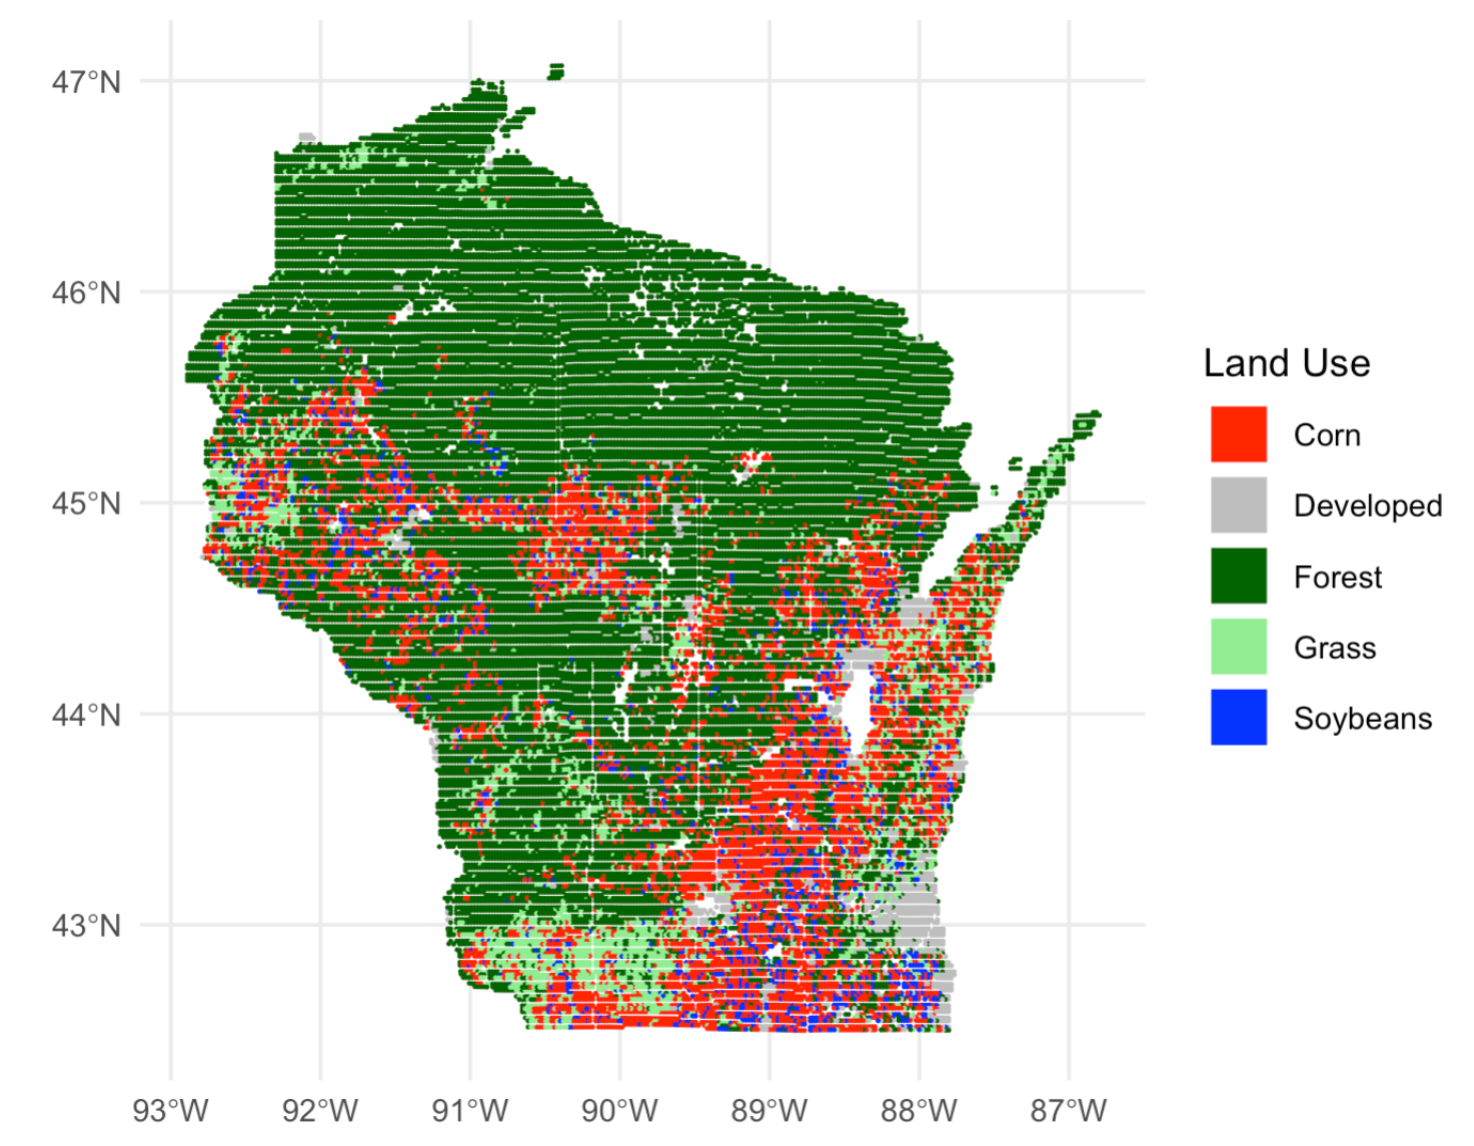
\includegraphics[width=0.6\linewidth]{spatial-land-use.png}
    \caption{Land use mapping in Wisconsin}
    \label{fig:land-use}
\end{figure}

\subsubsection{Precipitation}
We use the \texttt{climateR} package to obtain daily precipitation in Wisconsin from 2013 to 2023 and take the average precipitation at each monitoring site. The resolution of the precipitation monitoring sites is smaller than the PLSS grid. We use the bilinear interpolation to get the precipitation of each PLSS section. Figure \ref{fig:precipitation} shows the average precipitation mapping in Wisconsin.

\begin{figure}
    \centering
    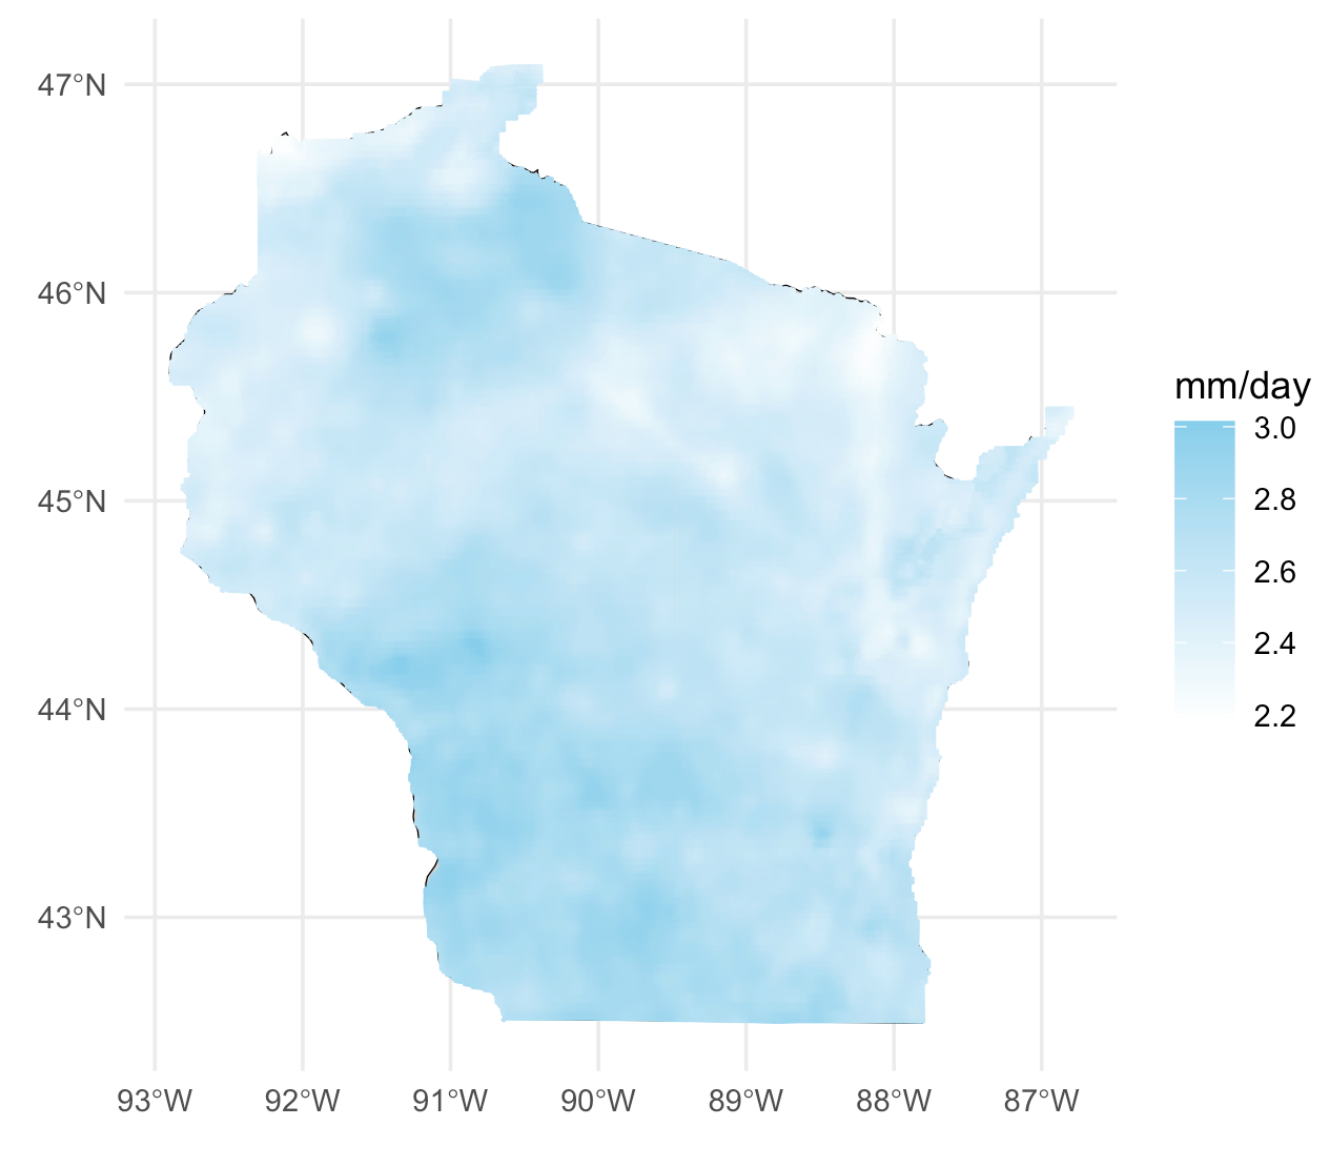
\includegraphics[width=0.6\linewidth]{precipitation.png}
    \caption{Average precipitation from 2013-2023 in Wisconsin}
    \label{fig:precipitation}
\end{figure}

\subsubsection{Soil Drainage}
The gridded National Soil Survey Geographic Database (gNATSGO) is a USDA-NRCS Soil and Plant Science Division (SPSD) composite database that provides complete coverage of the best available soils information for all areas of the United States and Island Territories. We use the \texttt{soilDB} package to download the soil drainage properties of Wisconsin. There are seven drainage levels, very poorly drained, poorly drained, somewhat poorly drained, moderately well drained, well drained, somewhat excessively drained, and excessively drained. The basic unit of gNATSGO is \textit{mapunit}. Each mapunit corresponds to one drainage level. For every PLSS section, we collect all the mapunits that overlap with the section and then assign the drainage level that dominates the PLSS section as its value of ``soil drainage''. Figure \ref{fig:drainage} shows the soil drainage mapping in Wisconsin.

\begin{figure}
    \centering
    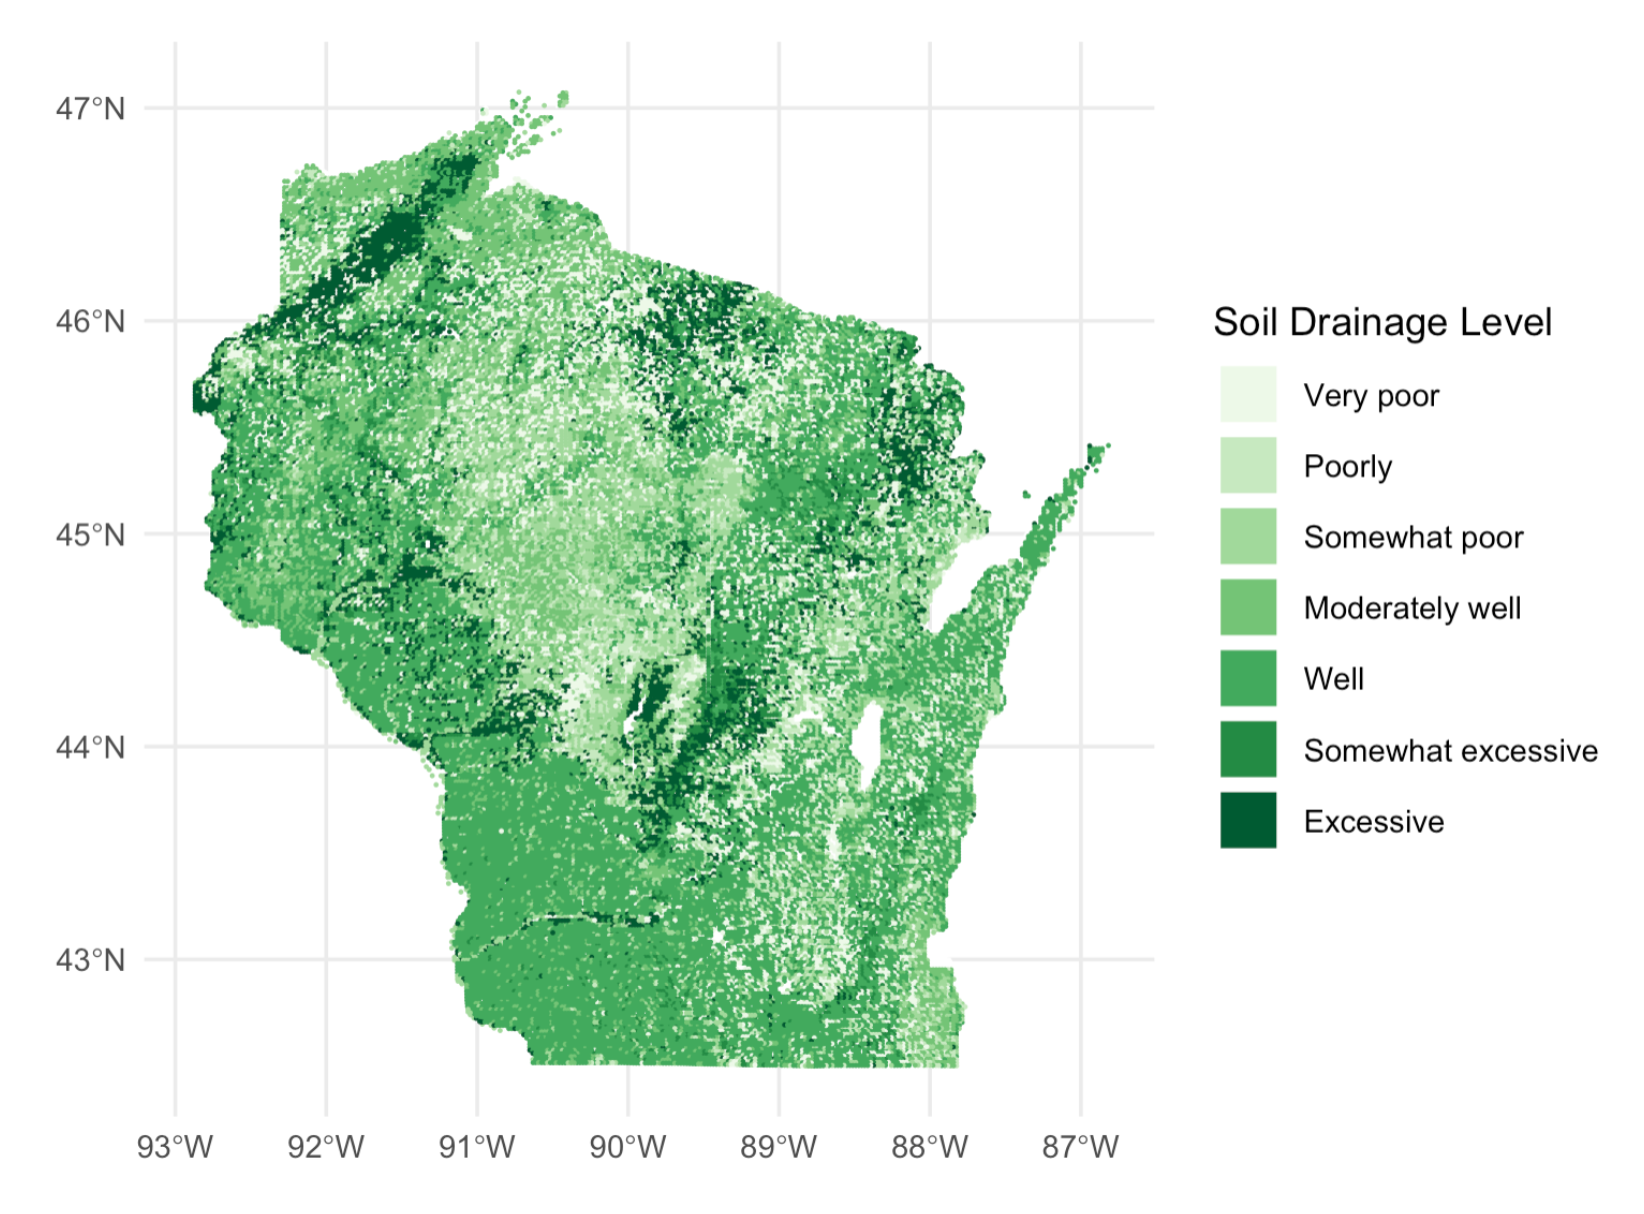
\includegraphics[width=0.7\linewidth]{drainage.png}
    \caption{Soil drainage mapping in Wisconsin}
    \label{fig:drainage}
\end{figure}


\subsubsection{Concentrated animal feeding operation (CAFO)}

While Wisconsin is famous for its dairy industry, the manure application at large farms as CAFOs (Concentrated Animal Feeding Operations) can produce nitrate. To consider the effect of livestock manure, we use the DNR-approved Wisconsin Pollutant Discharge Elimination System (WPDES) permit to construct the ``CAFO'' covariate. Each permit records the animal type, the number of the animal, and the PLSS location of the farm. Different animals produce different amounts of nitrate. United States Department of Agriculture (USDA) provides a reference to account for the nitrate load of different animal types (See Table \ref{tab:CAFO}).

\begin{table}[ht]
\centering
\begin{tabular}{l l}
\toprule
\textbf{Animal Type} & \textbf{Scaled Factor} \\ \midrule
Dairy & 5.1 \\ \hline
Turkeys & 18.0 \\ \hline
Swine & 4.0 \\ \hline
Sheep & 1.1 \\ \hline
Beef & 4.4 \\ \hline
Chickens & 17.1 \\ \hline
Ducks & 9.8 \\ 
\bottomrule
\end{tabular}
\caption{Nirate load of different animal types in CAFO.}
\label{tab:CAFO}
\end{table}
Since the animal manure can also affect the groundwater in nearby areas as well. We assume the effect of CAFO decreases quadratically with the distance and set the maximum distance to 10 kilometers. The, the effect of each CAFO permit is calculated as
$$\text{CAFO}=\text{Scaled Factor} \times \text{Animal Unit} \times\left(1- \left(\frac{\text{Distance}}{{\text{Max Distance}}}\right)^2\right).$$
Figure \ref{fig:cafo} shows the locations of CAFO in Wisconsin. Each circle in the map present a CAFO permit. The radius of the circle is 10 kilometers. The center of each circle has the highest value, i.e., animal unit multiplied by the scaled factor, and the value decreases quadratically from the center to the boundary of the circle.

\begin{figure}
    \centering
    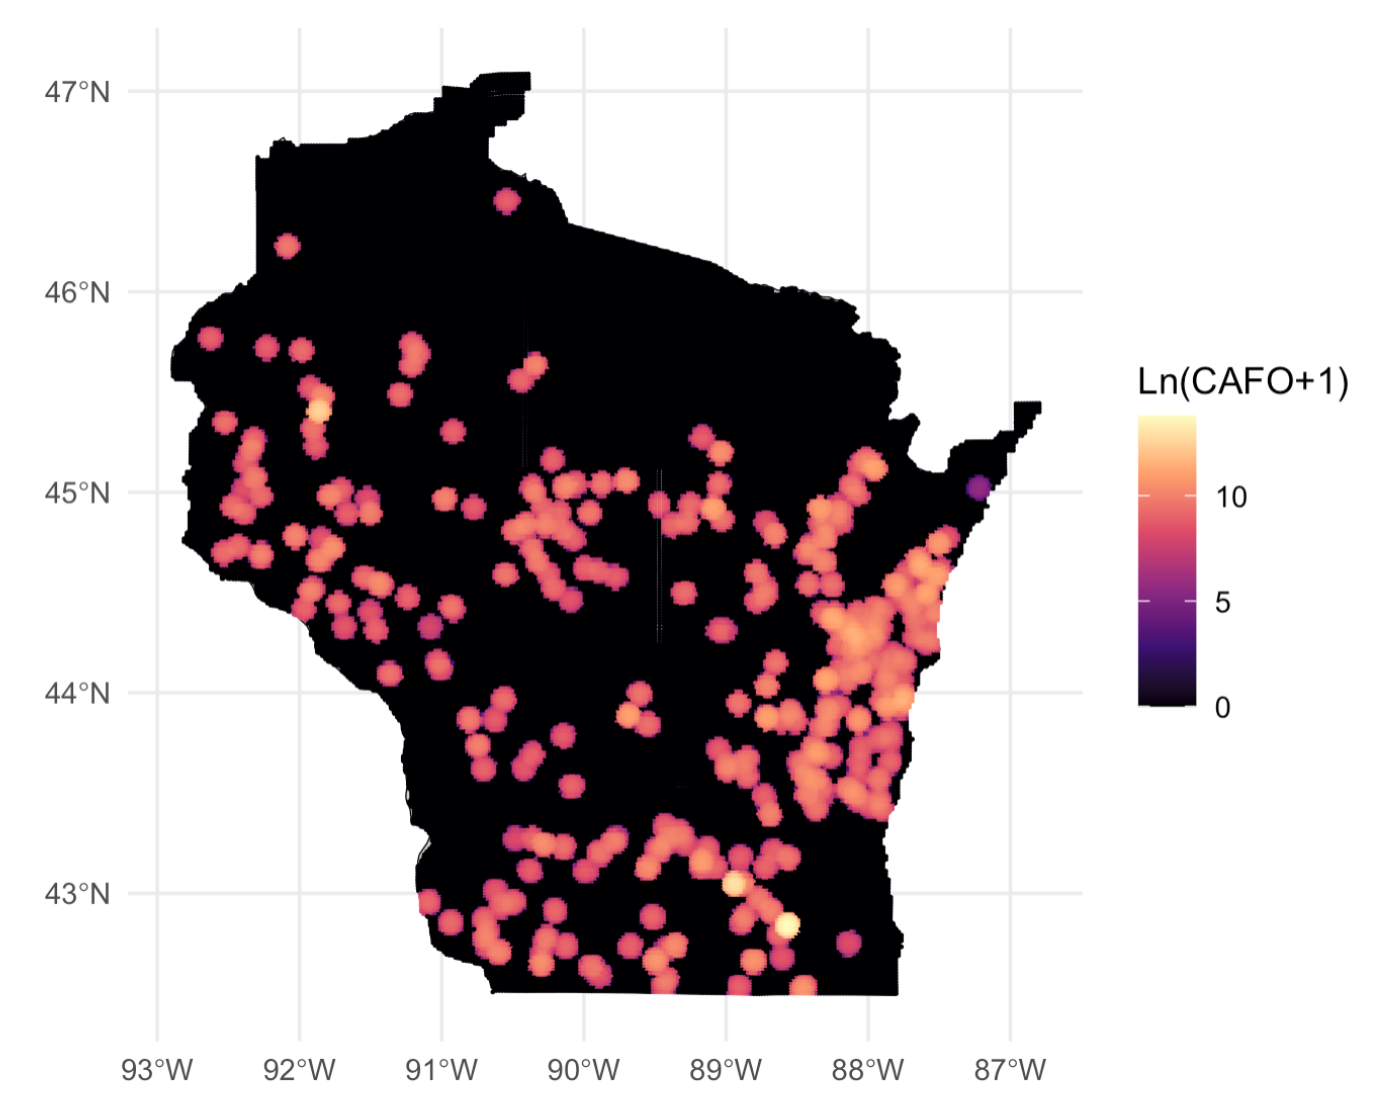
\includegraphics[width=0.6\linewidth]{cafo.png}
    \caption{CAFO in Wisconsin}
    \label{fig:cafo}
\end{figure}

\section{Computational Details of the Main Paper}	\label{sec:A}

\subsection{Leave-one-out Kriging}\label{sec:leave-one-out kriging}

To calculate the loss function \eqref{eq:loss_function_complete}, we must perform kriging as defined in Step \ref{step:kriging} for every observation $i$ given all other observations. This requires computing  $\hat\E[U_i|\textbf{U}_{-i}] = \mathbf{C}_{i}(\hat\psi)\mathbf{C}^{-1}_{-i}(\hat\psi)\hat{\textbf{U}}_{-i}$ for $i = 1,\ldots,n$. However, A straightforward implementation of this is computationally prohibitive because it requires inverting $n$ distinct $(n-1) \times (n-1)$ covariance sub-matrices, one for each observation $i$. We call this task \textit{leave-one-out kriging} and propose an efficient algorithm to avoid the computational redundancy.


Let $\Lambda$ be the precision matrix of the Gaussian process $\{U_i\}_{i=1}^n$, i.e., the inverse of covariance matrix. Let $T_i$ be the permutation matrix that swaps the first and $i$-th rows. The precision matrix for the permuted locations $T_i \Lambda T_i$ has the block structure:
$$ T_i \Lambda T_i = 
\left[
\begin{matrix}
    \Lambda_{i,i} & \Lambda_{i,-i}\\
    \Lambda_{-i,i} & \Lambda_{-i,-i}
\end{matrix}
\right].$$
Here, $\Lambda_{i,i}$ is the scalar $i$-th diagonal entry of $\Lambda$, and $\Lambda_{i,-i}$ is the $1 \times (n-1)$ row vector corresponding to the $i$-th row of $\Lambda$ (excluding the $i$-th column). Then, we use the properties of block matrix inversion (i.e., \href{https://en.wikipedia.org/wiki/Schur_complement}{Schur complement}) to find a direct relationship between the kriging weights and the blocks of the precision matrix: 
\begin{equation}\label{eq:schur_conditional}
   \mathbf{C}_{i}(\hat\psi)\mathbf{C}^{-1}_{-i}(\hat\psi) = -\Lambda_{i,i}^{-1}\Lambda_{i,-i} 
\end{equation}
The above equation implies that we only need to compute the precision matrix $\Lambda$ once to find the terms for all $n$ conditional expectations, rather than performing $n$ matrix inversions. 



\subsection{Vecchia Approximation}

The computation of the precision of the Gaussian processes $\{U_i\}_{i=1}^n$ is a crucial part of our method. In Step \ref{step:covariance_estimation}, maximum likelihood estimation involves the calculation of the precision. In Step \ref{step:kriging}, the kriging also involves the  calculation of the precision matrix. However, the precision matrix $\Lambda$ arising from Gaussian process are dense for large $n$, evaluating $\Lambda$ even once still incurs the computational cost of $O(n^3)$ and storage cost of $O(n^2)$ both of which are taxing on typical personal computing resources. Thankfully, there is a rich literature concerning the numerical approximation and fast computation of Gaussian processes. In our method, we employ the the Vecchia approximation \citep{vecchia1988estimation, katzfuss2021general} which can be implemented by the R package \citep{guinness2021gpgp}.

\subsection{DC Algorithm}\label{sec:dc_algorithm}

We use the difference of convex functions (DC) algorithm \citep{DCalgorithm} to efficiently solve the nonconvex objective function in \eqref{eq:loss_function_complete} is nonconvex. We decompose the loss function in equation \eqref{eq:loss_function_complete} into the difference of two convex function $L^{(\delta)+}(t,O_i)$ and $L^{(\delta)-}(t,O_i)$, i.e., $L^{(\delta)}(t,O_i) = L^{(\delta)+}(t,O_i) - L^{(\delta)-}(t,O_i)$ for any $a$
 and $O_i$ where
$$ L^{(\delta)+}(t,O_i) =
\begin{cases}
    \begin{aligned}
        \nu^{+}(a_L, O_i) &+ \epsilon -\epsilon \left\{\log( e + a_L- t)\right\}^{-1} \\
                         & + \tilde{\epsilon} (t-a_L)^2 + \nabla v^{-}(a_L,O_i)(t-a_L)
    \end{aligned}
    & \text{if } t < a_L \\
    \\
    \nu^{+}(t, O_i)
    & \text{if } a_L\leq t\leq a_U \\
    \\
    \begin{aligned}
        \nu^{+}(a_U, O_i) &+ \epsilon -\epsilon \left\{\log( e + t- a_U)\right\}^{-1} \\
                         & + \tilde{\epsilon} (t-a_U)^2 + \nabla v^{+}(a_U,O_i)(t-a_U)
    \end{aligned}
    & \text{if } t > a_U
\end{cases}
$$

$$ L^{(\delta)-}(t,O_i) = 
\begin{cases}
    \nu^{-}(a_L, O_i)+\tilde{\epsilon} (t-a_L)^2 + \nabla v^{-}(a_L,O_i)(t-a_L)& t<a_L\\
    \nu^{-}(t, O_i)& a_L\leq t\leq a_U\\
    \nu^{-}(a_U, O_i)+\tilde{\epsilon} (t-a_U)^2 + \nabla v^{+}(a_U,O_i)(t-a_U)& t> a_U
\end{cases}
$$


 When we define the decomposition component outside the range $[a_L, a_U]$. We include derivative of the loss decomposition component inside the treatment range, i.e., $\nu^{+}(t, O_i)$ and $\nu^{-}(t, O_i)$, at the boundary so that the function we defined outside the range guarantees the convexity. Specifically, $\epsilon$ need to be large enough to guarantee that loss function converge fast outside the boundary. $\bar\epsilon$ need to be large enough to ensure the convexity of $L^{+}$.

Then, we discuss the decomposition of the loss function when $a\in[a_L,a_U]$. For the clarity of the notation, we define
$$r_i:=\frac{(Y_i - \mu(A_i,X_i,S_i))K_\delta(A_i-a)}{p(A_{i}|X_{i},S_{i})}.$$
$$\Psi(a) := \int_{a_L}^a K_\delta(A_i-a^\prime)\mathrm{d}a^\prime,\quad a\in[a_L,a_U].$$
Then, $\nu^{(\delta)}(a,O_i)$ in \eqref{eq:loss_function_bounded} can be written as 
$$\nu^{(\delta)}(a, O_i) 
   = 
   \mathcal{T}(a-a_L) -\int_{a_L}^a\mu(a^\prime,O_i)\mathrm{d}a^\prime - r_i\Psi(a) + C_0,\quad t\in[a_L,a_U]$$
In the right-hand-side of the above equation, $\mathcal{T}(a-a_L) -\int_{a_L}^a\mu(a^\prime,O_i)\mathrm{d}a^\prime$ is a convex function of $a$ so we only need to decompose $\Psi(a)$ as the difference of two convex function. In our method, we consider a Gaussian kernel 
$$K_\delta(A_i-a) = \frac{1}{\sqrt{2\pi}\delta} \exp\left(-\frac{1}{2\delta^2}(A_i-a)^2\right),\quad a\in[a_L,a_U].$$
The second order derivative of $\Psi(a)$ is
$$\Psi^{\prime\prime}(a)=-\frac{1}{\sqrt{2\pi}\delta} \exp\left(-\frac{1}{2\delta^2}(a-A_i)^2\right)\frac{1}{\delta^2}(a-A_i),\quad t\in[a_L,a_U].$$
A lower bound of its second-order derivative
\begin{align*}
\inf_{a\in\R}\Psi^{\prime\prime}(a)&= \inf_{a\in\R}\left[-\frac{1}{\sqrt{2\pi}\delta} \exp\left(-\frac{1}{2\delta^2}(a-A_i)^2\right)\frac{1}{\delta^2}(a-A_i)\right]\\
&=\inf_{m\in\R}\left[-\frac{1}{\sqrt{\pi}\delta^2} \exp\left(-m^2\right)m\right]\\
&=\frac{1}{\sqrt{\pi}\delta^2} \exp\left(-\frac{1}{2}\right)(-1/\sqrt{2})\\
& := -\frac{\alpha}{\delta^2}
\end{align*}
Here, $\alpha:=\frac{1}{\sqrt{\pi}} \exp\left(1/2\right)(-1/\sqrt{2})$. Then, $\Psi(a) = \Psi^{+}(a) - \Psi^{}(a)$ where
\begin{gather*}
    \Psi^{+}(a):=\int_{a_L}^a K_\delta(A_i-a^\prime)\mathrm{d}a^\prime +\int_{a_L}^a \frac{\alpha a^\prime}{\delta^2}\mathrm{d}a^\prime,\quad a\in[a_L,a_U] \\
    \Psi^{-}(a):=\int_{a_L}^a \frac{\alpha a^\prime}{\delta^2}\mathrm{d}a^\prime,\quad a\in[a_L,a_U] \\
\end{gather*}
 Let $r_i^{+} = \max(r_i, 0)$, $r_i^{-} = -\min(r_i, 0)$. Then, we have the decomposition of the loss function for $a\in[a_L,a_U]$:
\begin{gather*}
\nu^{(\delta)}(a, O_i) = \nu^{(\delta)+}(a, O_i) - \nu^{(\delta)-}(a, O_i)\\
    \nu^{(\delta)+}(a, O_i) 
   = \mathcal{T}(a-a_L) -\int_{a_L}^a\mu(a^\prime,O_i)\mathrm{d}a^\prime + r_i^{+}\Psi^{-}(a)+ r_i^{-}\Psi^{+}(t)\\
    \nu^{(\delta)-}(a, O_i) 
   = r_i^{+}\Psi^{+}(a)+ r_i^{-}\Psi^{-}(a) ,\quad a\in[a_L,a_U]
\end{gather*}





\section{Proof of Lemmas and Theorems}\label{sec:B}

\subsection{Proof of Theorem \ref{thm:execess_risk}}
We start the proof with the definition of some new notation. First, similar to \eqref{eq:loss_function_complete}, we define the estimated loss function where the nuisance parameters are substituted by their estimation:
\begin{subequations}
    \begin{equation*}
        \widehat L^{(\delta)}(a,O_i) = \begin{cases}
    \widehat\nu^{(\delta)}(a_L, O_i)+\epsilon -\epsilon \left\{\log( e + a_L- a)\right\}^{-1}& \text{if } -\infty<a<a_L\\
    \widehat\nu^{(\delta)}(a, O_i)&\text{if }  a_L\leq a\leq a_U\\
    \widehat\nu^{(\delta)}(a_U, O_i)+\epsilon -\epsilon \left\{\log( e + a- a_U)\right\}^{-1}&\text{if }  a_U<t< \infty
\end{cases}
    \end{equation*}
    \begin{equation*}
        \widehat\nu^{(\delta)}(a, O_i) = \int_{\mathcal{A}} (\mathcal{T} - \widehat\psi^{(\delta)}(a^\prime,O_i))1(a^\prime\leq a)\mathrm{d}a^\prime + C_0.
    \end{equation*}
\begin{equation*}
    \widehat\psi^{(\delta)}(a,O_i) := \hat\mu(a,X_i,S_i)+ \frac{(Y_i - \hat\mu(A_i,X_i,S_i))K_\delta(A_i-a)}{\hat p(A_{i}|X_{i},S_{i})}.
\end{equation*}
\end{subequations}
Additionally, we define the true loss function where the pseudo outcome is subtituted by the true outcome regression:

\begin{subequations}
    \begin{equation*}
         L(a,O_i) = \begin{cases}
    \nu(a_L, O_i)+\epsilon -\epsilon \left\{\log( e + a_L- a)\right\}^{-1}& \text{if } -\infty<a<a_L\\
    \nu(a, O_i)&\text{if }  a_L\leq a\leq a_U\\
    \nu(a_U, O_i)+\epsilon -\epsilon \left\{\log( e + a- a_U)\right\}^{-1}&\text{if }  a_U<t< \infty
\end{cases}
    \end{equation*}
    \begin{equation*}
        \nu(a, O_i) = \int_{\mathcal{A}} (\mathcal{T} - \mu^*(a^\prime,O_i))1(a^\prime\leq a)\mathrm{d}a^\prime + C_0.
    \end{equation*}
\end{subequations}
Then, we define the intermediate quantities used to establish the the execess risk:
\begin{gather*}
   \widehat R_n^{(\delta)}(\theta) = \sum_{i=1}^n\widehat L^{(\delta)}(\theta(S_i),O_i),\quad
   \widehat R^{(\delta)}(\theta) = \E[\widehat L^{(\delta)}(\theta(S_i),O_i)],\\
   R^{(\delta)}(\theta) = \E[ L^{(\delta)}(\theta(S_i),O_i)],\quad
   R(\theta) = \lim_{\delta\rightarrow 0}\E[L^{(\delta)}(\theta(S_i),O_i)],\\
   \hat\theta = \arg\min_{\theta\in\mathcal{H}_{\gamma_n}} \widehat R_n^{(\delta)}(\theta),\quad \tilde\theta = \arg\min_{\theta\in\Theta} \widehat R^{(\delta)}(\theta), \quad
   \theta^* = \arg\min_{\theta\in\Theta}  R(\theta)
\end{gather*}
Given the above definitions, we decompose the excess risk as follows:
$$|R(\hat\theta)-R\left(\theta^*\right)|\leq \underbrace{|R(\hat\theta)-\widehat R^{(\delta)}(\hat\theta)|}_{\text{Term (A)}} + \underbrace{|\widehat R^{(\delta)}(\hat\theta) - \widehat R^{(\delta)}(\tilde\theta)|}_{\text{Term (B)}} + \underbrace{|\widehat R^{(\delta)}(\tilde\theta) - R(\theta^*)|}_{\text{Term (C)}}$$
By Lemma \ref{lemma:risk_function_plug_in_error}, term (A) has the upper bound with probability $1-\Delta_n$:
$$|R(\hat\theta)-\widehat R^{(\delta)}(\hat\theta)|\leq |\mathcal{A}|\left(\frac{2C^{\prime2}}{c^{\prime2}}\delta + \frac{1}{c^\prime}r_{\mu,n}r_{p,n} + C^\prime r_{\mu,n}\delta\right). $$
Since $\tilde\theta$ is the minimizer of $\widehat R^{(\delta)}(\theta)$ and $\theta^*$ is the minimizer of $R(\theta)$, we have the following upper bound of term (C) with probability $1-\Delta_n$:
\begin{align*}
    |\widehat R^{(\delta)}(\tilde\theta) - R(\theta^*)|\leq &\max\left\{|\widehat R^{(\delta)}(\theta^*) - R(\theta^*)|,|\widehat R^{(\delta)}(\tilde\theta) - R(\tilde\theta)|\right\} \\
    \leq &|\mathcal{A}|\left(\frac{2C^{\prime2}}{c^{\prime2}}\delta + \frac{1}{c^\prime}r_{\mu,n}r_{p,n} + C^\prime r_{\mu,n}\delta\right)
\end{align*}
By Lemma \ref{lemma:svm_estimation_error}, term (B) has the following bound with probability $1-32e^{-\tau}$,
\begin{align*}
   \widehat R^{(\delta)}(\hat\theta) - \widehat R^{(\delta)}(\tilde\theta)\leq & c_1 \lambda_n\gamma_n^{-d} + c_2\gamma_n^{\beta}+ c_3\delta^{-\frac{1}{2}}\left(\gamma_n^{-d}\lambda_n^{-p}n^{-1}\sigma\right)^{\frac{1}{2+2p}} + \\
   &\qquad + c_4n^{-1} + c_5\ln(n)\sigma^{\frac{1}{2}}\delta^{-\frac{1}{2}}n^{-\frac{1}{2}} + c_6(\tau \sigma)^{\frac{1}{2}} n^{-\frac{1}{2}}\delta^{-\frac{1}{2}}
\end{align*}
Combing the results above, we have that with probability $1-32e^{-\tau} - \Delta_n$,
\begin{align*}
       |R(\hat\theta)-R\left(\theta^*\right)|\leq & c_1 \lambda_n\gamma_n^{-d} + c_2\gamma_n^{\beta}+ c_3\delta^{-\frac{1}{2}}\left(\gamma_n^{-d}\lambda_n^{-p}n^{-1}\sigma\right)^{\frac{1}{2+2p}} + \\
   &\qquad + c_4n^{-1} + c_5\ln(n)\sigma^{\frac{1}{2}}\delta^{-\frac{1}{2}}n^{-\frac{1}{2}} + c_6(\tau \sigma)^{\frac{1}{2}} n^{-\frac{1}{2}}\delta^{-\frac{1}{2}}\\
       & \qquad\qquad + c_7r_{\mu,n}r_{p,n} + c_8 r_{\mu,n}\delta + c_9\delta
    \end{align*}
If we further let $\lambda_n \propto (\sigma^{-1}n\delta)^{-\frac{d+\beta}{2\beta + d}}$ and $\gamma_n\propto (\sigma_n^{-1}n\delta)^{-\frac{1}{2\beta + d}}$. The rates will be further simplified to 
\begin{align*}
       |R(\hat\theta)-R\left(\theta^*\right)|\leq & c_1(\sigma_n^{-1}n\delta)^{-\frac{\beta}{2\beta + d}} + c_2n^{-1} + c_3\ln(n)\sigma^{\frac{1}{2}}\delta^{-\frac{1}{2}}n^{-\frac{1}{2}} \\
   &\qquad  + c_4(\tau \sigma)^{\frac{1}{2}} n^{-\frac{1}{2}}\delta^{-\frac{1}{2}} + c_5r_{\mu,n}r_{p,n} + c_6 r_{\mu,n}\delta + c_9\delta
    \end{align*}
In the above rate, terms $c_2n^{-1} + c_3\ln(n)\sigma^{\frac{1}{2}}\delta^{-\frac{1}{2}}n^{-\frac{1}{2}} + c_4(\tau \sigma)^{\frac{1}{2}} n^{-\frac{1}{2}}\delta^{-\frac{1}{2}} $ converge faster than the term $c_1(\sigma_n^{-1}n\delta)^{-\frac{\beta}{2\beta + d}}$. Additionally, since $r_{\mu,n}=o(1)$, we can omit the term $r_{\mu,n}\delta$ as well. Therefore, we have the following high probability rate for the execess risk bound:
$$R(\hat\theta)-R\left(\theta^*\right) = O_P\left\{(\sigma^{-1}\delta n)^{-\frac{\beta}{2\beta + d}}+r_{\mu,n}r_{p,n} +\delta\right\}.$$
Suppose $\sigma_n=O(1)$. Then, for fixed $\beta,d$, if we let $\delta\propto n^{-\beta/(3\beta + d)}$. The final rate would become $n^{-\beta/(3\beta + d)}$.

\subsection{Proof of Useful Lemmas}

\begin{lemma}\label{lemma:svm_estimation_error}
    Suppose that $\tilde\theta$ belongs to a a Besov space on $\R^d$ with smoothness parameter $\beta>0$, i.e., $\mathcal{B}_{1,\infty}^\beta(\R^d) = \{f\in L_\infty(\R^d)|\sup_{t>0}t^{-\beta\{\omega_{r,L_1(\R^d)}(f,t)\}}\}$ where $\omega_r$ is the modulus of continuity of order $r$. Then, for $p\in(0,1]$, we have the following execess risk bound for $\hat\theta$ with probability $1-32e^{-\tau}$:
   \begin{align*}
   \widehat R^{(\delta)}(\hat\theta) - \widehat R^{(\delta)}(\tilde\theta)\leq & c_1 \lambda_n\gamma_n^{-d} + c_2\gamma_n^{\beta}+ c_3\delta^{-\frac{1}{2}}\left(\gamma_n^{-d}\lambda_n^{-p}n^{-1}\sigma\right)^{\frac{1}{2+2p}} + \\
   &\qquad + c_4n^{-1} + c_5\ln(n)\sigma^{\frac{1}{2}}\delta^{-\frac{1}{2}}n^{-\frac{1}{2}} + c_6(\tau \sigma)^{\frac{1}{2}} n^{-\frac{1}{2}}\delta^{-\frac{1}{2}}
\end{align*}
    
\end{lemma}

\begin{proof}

Let $\theta_0$ be any fixed element in RKHS $\mathcal{H}_{\gamma_n}$.
    \begin{align*}
   &\widehat R^{(\delta)}(\hat\theta) - \widehat R^{(\delta)}(\tilde\theta)\\
   = & \lambda_n\|\hat\theta\|_{\mathcal{H}_{\gamma_n}}+ \widehat R_n^{(\delta)}(\hat\theta)+\widehat R^{(\delta)}(\hat\theta)  - \widehat R_n^{(\delta)}(\hat\theta) - \widehat R^{(\delta)}(\tilde\theta)\\
   \leq & \lambda_n\|\theta_0\|_{\mathcal{H}_{\gamma_n}}  + \widehat R_n^{(\delta)}(\theta_0)+ \widehat R^{(\delta)}(\hat\theta) - \widehat R_n^{(\delta)}(\hat\theta) - \widehat R^{(\delta)}(\tilde\theta)\\
   \leq & \lambda_n\|\theta_0\|_{\mathcal{H}_{\gamma_n}}+\widehat R^{(\delta)}(\theta_0) -\widehat R^{(\delta)}(\tilde\theta) + \widehat R_n^{(\delta)}(\theta_0) - \widehat R^{(\delta)}(\theta_0) +
   \widehat R^{(\delta)}(\hat\theta)
     -\widehat R_n^{(\delta)}(\hat\theta) \\
   \leq & \underbrace{\left|\lambda_n\|\theta_0\|_{\mathcal{H}_{\gamma_n}}+\widehat R^{(\delta)}(\theta_0) -\widehat R^{(\delta)}(\tilde\theta)\right|}_{\text{Term (A)}} + \underbrace{\left|\widehat R_n^{(\delta)}(\theta_0) - \widehat R^{(\delta)}(\theta_0)\right|}_{\text{Term (B)}} + \underbrace{
   \left|\widehat R^{(\delta)}(\hat\theta)
     -\widehat R_n^{(\delta)}(\hat\theta)\right|}_{\text{Term  (C)}}
\end{align*}
In the last inequality above, term (A) is the approximation error term. Term (B) is the deviation error since $\theta_0$ is fixed. Term (C) is the empirical error term because $\hat\theta$. We also note that $\hat R$ depends on nuisance estimation $\hat\mu,\hat p$, which is not independent with the expectation taken over the loss function because we do not implement cross-fitting.


\noindent\textbf{Bounding Term (A):} 

\noindent In order bound (A), we construct a $\theta_0\in\mathcal{H}_{\gamma_n}$ to make both the regularization $\lambda_n\|\theta_0\|_{\mathcal{H}_{\gamma_n}}$ and the approximation error $\widehat R^{(\delta)}(\theta_0) -\widehat R^{(\delta)}(\tilde\theta)$ reasonably small. Here, $d$ is the dimension of $(X_i,U_i)$. For the brevity of the proof, we omit $U_i$ in the notation. For example, we omit $u$ in $\theta_0(x,u)$ and only use $\theta_0(x)$. 

For $r\in\{1,2,\ldots\}$ and $\gamma>0$, function $Q_{r,\gamma}: \mathbb{R}^d \to \mathbb{R}$ as
\begin{equation} \label{eq:eberts_Q_r}
Q_{r,\gamma}(x) = \sum_{j=1}^r \binom{r}{j}(-1)^{j-1} \frac{1}{j^d} \left(\frac{2}{\gamma^2}\right)^{\frac{d}{2}} \mathcal{K}_{j\gamma/\sqrt{2}}(z), \quad \mathcal{K}_{\gamma}(x) = \exp\{-\gamma^{-2} \|x\|_2^2\}
\end{equation}
The support of $\tilde\theta$ is finite and $\tilde\theta$ is bounded, we have $\tilde\theta \in L_2(\mathbb{R}^d) \cap L_\infty(\mathbb{R}^d)$. Then, we define $\theta_0$ by convolving $Q_{r,\gamma}$ with $\tilde\theta$, that is
\[
\theta_0(x) = (Q_{r,\gamma} * \tilde\theta_{L,\pr})(x) := \int_{\mathbb{R}^d} Q_{r,\gamma}(x - z) \tilde\theta_{L,\pr}(z) \mathrm{d}z.
\]
Let $\pr_X$ be the distribution of $X$ and $g_X$ be the density function. We assume $g_X\in L_\infty(\R^d)$. Applying Lemma \ref{lemma:thm2.2_eberts} while specifying $p=\infty,s=1,q=1$, we have
\begin{equation}\label{eq:approx_error_execess_risk}
    \|Q_{r,\gamma} * \tilde\theta - \tilde\theta\|_{L_1(\pr_X)} \le C_{r,1} \|g_X\|_{L_\infty(\mathbb{R}^d)} \omega_{r,L_{1}(\mathbb{R}^d)}(\tilde\theta, \gamma/2)
\end{equation}
Additionally, by Lemma \ref{lemma:thm2.3_eberts}, 
\begin{equation}\label{eq:approx_error_regularizer}
    \|\theta_0\|_{\mathcal{H}_{\gamma_n}} = \|Q_{r,\gamma} * \tilde\theta\|_{\mathcal{H}_{\gamma_n}}\leq (\gamma\sqrt{\pi})^{-\frac{d}{2}}(2^r-1)\|\tilde\theta\|_{L_2(\R^d)}.
\end{equation}
Finally, we derive the Lipschitz properties of $\widehat R^{\delta}(\theta)$ with respective to $\theta$.
    \begin{equation*}
        \nabla_a\E\left[\widehat L^{(\delta)}(a,O_i)\right] = \begin{cases}
     -\epsilon \frac{\partial}{\partial a}\left\{\log( e + a_L- a)\right\}^{-1}& \text{if } -\infty<a<a_L\\
    \mathcal{T} - \E\left[\hat\mu(a,X_i,S_i)+ \frac{(Y_i - \hat\mu(A_i,X_i,S_i))K_\delta(A_i-a)}{\hat p(A_{i}|X_{i},S_{i})}\right]&\text{if }  a_L\leq a\leq a_U\\
     -\epsilon \frac{\partial}{\partial a}\left\{\log( e + a- a_U)\right\}^{-1}&\text{if }  a_U<t< \infty
\end{cases}
    \end{equation*}
Thus, we have
\begin{equation}\label{eq:approx_error_derivative_bound}
   \nabla_a\E\left[\widehat L^{(\delta)}(a,O_i)\right]\leq 2C^\prime c^{\prime-1}\delta^{-1}\kappa +\mathcal{T} + C^\prime 
\end{equation}
Combine \eqref{eq:approx_error_execess_risk}, \eqref{eq:approx_error_regularizer} and \eqref{eq:approx_error_derivative_bound}, we have
\begin{align}
&\lambda_n\|\theta_0\|_{\mathcal{H}_{\gamma_n}}+\widehat R^{(\delta)}(\theta_0) -\widehat R^{(\delta)}(\tilde\theta)\nonumber\\
    =& \lambda_n \|Q_{r,\gamma} * \tilde\theta\|_{\mathcal{H}_{\gamma_n}} + \widehat R^{(\delta)}(Q_{r,\gamma} * \tilde\theta) -\widehat R^{(\delta)}(\tilde\theta)\nonumber\\
    \le{}& \lambda_n (\gamma_n\sqrt{\pi})^{-d}(2^r - 1)^2 \|\tilde\theta\|_{L_2(\mathbb{R}^d)}^2 +  (2C^\prime c^{\prime-1}\delta^{-1}\kappa +\mathcal{T} + C^\prime)\|Q_{r,\gamma_n} * \tilde\theta - \tilde\theta\|_{L_1(P_X)}^2 \nonumber\\
    \le{}& \lambda_n (\gamma_n\sqrt{\pi})^{-d}(2^r - 1)^2 \|\tilde\theta\|_{L_2(\mathbb{R}^d)}^2 +  C_{r,1} (2C^\prime c^{\prime-1}\delta^{-1}\kappa +\mathcal{T} + C^\prime)\|g_X\|_{L_\infty(\mathbb{R}^d)} \omega_{r,L_{1}(\mathbb{R}^d)}(\tilde\theta, \gamma_n/2)\nonumber\\
    \le{} & \lambda_n (\gamma_n\sqrt{\pi})^{-d}(2^r - 1)^2 \|\tilde\theta\|_{L_2(\mathbb{R}^d)}^2 +  C_{r,1} (2C^\prime c^{\prime-1}\delta^{-1}\kappa +\mathcal{T} + C^\prime)\|g_X\|_{L_\infty(\mathbb{R}^d)} \gamma_n^\beta\\
    \leq & c_1 \lambda_n\gamma_n^{-d} + c_2(\delta^{-1}+1)\gamma_n^{\beta}
    \label{eq:approx_error_svm}
\end{align} 

\noindent
\textbf{Bounding Term (B):}

\noindent We use concentration inequality in Lemma \ref{lemma:gaussian_concentration} to bound term (B). We let $\mathcal{F}_\mu$ be the function class of $\hat\mu$, and $\mathcal{F}_p$ be the function class of $\hat p$. Let us now fix a minimal $\epsilon_\mu$-net $\mathcal{C}_\mu$ of the function class $\mathcal{F}_\mu$, and a minimal $\epsilon_p$-net $\mathcal{C}_p$ of the function class $\mathcal{F}_p$. By the union bound, 
\begin{align}
&\pr\left(\sup_{\mu\in\mathcal{C}_\mu, p\in \mathcal{C}_p}\left|R_n^{(\delta)}(\theta_0;\mu, p)-R^{(\delta)}(\theta_0;\mu, p)\right|\geq t\right)\nonumber\\
\leq & |\mathcal{C}_\mu||\mathcal{C}_p|\max_{\mu\in\mathcal{C}_\mu, p\in \mathcal{C}_p}\pr\left(\left|R_n^{(\delta)}(\theta_0;\mu, p)-R^{(\delta)}(\theta_0;\mu, p)\right|\geq t\right)\nonumber\\
\leq &
8|\mathcal{C}_\mu||\mathcal{C}_p|\exp\left(-\frac{cnt^2\delta}{\sigma}\right)\nonumber
\end{align}
A transformation yields that, with probability no less than $1-8|\mathcal{C}_\mu||\mathcal{C}_p|e^{-\tau}$,
\begin{equation}\label{eq:union_bound}
   \sup_{\mu\in\mathcal{C}_\mu, p\in \mathcal{C}_p}\left|R_n^{(\delta)}(\theta_0;\mu, p)-R^{(\delta)}(\theta_0;\mu, p)\right|\leq \sqrt{\frac{\tau \sigma}{cn\delta}}. 
\end{equation}
For any $\mu,\mu^\prime$, both $R^{(\delta)}(\theta_0;\mu, p)$ is uniformly Lipschitz with respect to $\mu$,
\begin{align}
    &R^{(\delta)}(\theta_0;\mu, p) - R^{(\delta)}(\theta_0;\mu^\prime, p)\nonumber\\
     =  & \int_{a_L}^{\theta_0(X_i,U_i)}\E\left\{\mu(a,X_i,S_i) - \mu^\prime(a,X_i,S_i) + \frac{(\mu(A_i,X_i,S_i)- \mu^\prime(A_i,X_i,S_i))K_\delta(A_i-a)}{ p(A_{i}|X_{i},S_{i})}\right\}\mathrm{d}a\nonumber\\
     \leq & 
    c^{\prime-1} \E\left[\left|\mu(A_i,X_i,S_i) - \mu^\prime(A_i,X_i,S_i)\right|\right]\times \left(|\mathcal{A}| + \int_{a_L}^{\theta_0(X_i,U_i)}K_\delta(A_i-a)\mathrm{d}a\right)\nonumber\\
    \leq& (|\mathcal{A}| + 1)\times \|\mu(A_i,X_i,S_i) - \mu^\prime(A_i,X_i,S_i) \|_{P,2}\nonumber\\
    = & (\left|\mathcal{A}\right|+1)\|\mu - \mu^\prime \|_{P,2} \label{eq:lipschitz_to_mu_E}
\end{align}
To derive the Lipschitz property of $R_n^{(\delta)}(\theta_0;\mu, p)$, we need to derive additional concentration inequality. Under structural model \eqref{eq:dgp_1}, \eqref{eq:dgp_2}, $\mu$ is a function of multivariate Gaussian process $(X_i,U_i)$ with covariance matrix $\Sigma_n$ whose spectral norm is $\sigma$. Suppose $Z$ is an $d\times n$ dimension i.i.d. normal distribution. Then, under Assumption \ref{condition:excess_risk:boundedness}, $\E_n[\mu(X_i,U_i)-\mu^\prime(X_i,U_i)]$ is a Lipschitz function of $Z$ with Lipschitz factor scaled by $\sigma$. Thus, applying \ref{lemma:gaussian_concentration} to $\E_n[\mu(X_i,U_i)-\mu^\prime(X_i,U_i)]$ gives us,
\begin{equation*}
\pr\left(\left|\E_n\left[|\mu - \mu^\prime| \right]-\E\left[|\mu - \mu^\prime| \right]\right|\geq t\right)\leq \exp\left(-\frac{cnt^2}{\sigma}\right)
\end{equation*}
Then, for any $\mu,\mu^\prime$, both $R_n^{(\delta)}(\theta_0;\mu, p)$ is uniformly Lipschitz with respect to $\mu$ with probability no less than $1-e^{-\tau}$ as follows:
\begin{align}
    &R_n^{(\delta)}(\theta_0;\mu, p) - R_n^{(\delta)}(\theta_0;\mu^\prime, p)\nonumber\\
    \leq & (|\mathcal{A}| + 1)\E_n\left[|\mu - \mu^\prime| \right]\nonumber\\
    \leq & (|\mathcal{A}| + 1)\left(\E\left[|\mu - \mu^\prime|\right] + \sqrt{\frac{\tau \sigma}{cn}}\right)\nonumber\\
    \leq & (|\mathcal{A}| + 1)\left(\|\mu - \mu^\prime\|_{P,2} + \sqrt{\frac{\tau \sigma}{cn}}\right)
\label{eq:lipschitz_to_mu_En}
\end{align}
Similarly, for any $p,p^\prime$, we have the Lipschitz property of  $R^{(\delta)}(\theta_0;\mu, p)$ with respect to $p$ with probability no less than: 
\begin{equation}\label{eq:lipschitz_to_p_E}
    R^{(\delta)}(\theta_0;\mu, p) - R^{(\delta)}(\theta_0;\mu, p^\prime)\leq |\mathcal{A}|(2C^{\prime}c^{\prime-2})\|\hat p - p^\prime \|_{P,2},
\end{equation}
To derive the Lipschitz property of $R_n^{(\delta)}$,
we apply Lemma \ref{lemma:gaussian_concentration} to $\E_n\left[|p - p^\prime| \right]$,
\begin{equation*}
\pr\left(\left|\E_n\left[|p - p^\prime| \right]-\E\left[|p - p^\prime| \right]\right|\geq t\right)\leq \exp\left(-\frac{cnt^2}{\sigma}\right)
\end{equation*}
Then, we apply Chernoff bound to $\epsilon:=Y_i-\mu^*(A_i,X_i,S_i)$, which gives us 
$$\pr\left(\left|\E_n\left[\epsilon^2\right] ^{\frac{1}{2}} - \sigma_\epsilon\right|\geq t\right)\leq \exp\left(-\frac{nt^2}{\sigma_\epsilon^2}\right).$$
Combine the above two concentration inequality, for any $p,p^\prime$, we have the Lipschitz property of $R_n^{(\delta)}(\theta_0;\mu, p)$ with respect to $p$ with probability no less than $1-2e^{-\tau}$: 
\begin{align}
    &R_n^{(\delta)}(\theta_0;\mu, p) - R_n^{(\delta)}(\theta_0;\mu, p^\prime)\nonumber\\
    = & \frac{1}{2}\sum_{i=1}^n\int_{a_L}^{\theta_0(X_i,U_i)}  \frac{(Y_i -  \mu(A_i,X_i,S_i))K_\delta(A_i-a)}{ p(A_{i}|X_{i},S_{i})p^\prime(A_{i}|X_{i},S_{i})}\left(p^\prime(A_{i}|X_{i},S_{i}) -p(A_{i}|X_{i},S_{i})\right)\mathrm{d}a\nonumber\\
    \leq & |\mathcal{A}| \E_n\left[\left|\frac{(Y_i -  \mu(A_i,X_i,S_i))K_\delta(A_i-a)}{ p(A_{i}|X_{i},S_{i})p^\prime(A_{i}|X_{i},S_{i})}\right|^2\right]^{\frac{1}{2}} \E_n\left[\left|p^\prime(A_{i}|X_{i},S_{i}) -p(A_{i}|X_{i},S_{i})\right|^2\right]^{\frac{1}{2}}\nonumber\\
    \leq & |\mathcal{A}| c^{\prime-2}\kappa\delta^{-1}\left(2C^{\prime}+\E_n[\epsilon^2]^{\frac{1}{2}}\right)\E_n\left[\left|p^\prime(A_{i}|X_{i},S_{i}) -p(A_{i}|X_{i},S_{i})\right|^2\right]^{\frac{1}{2}}\nonumber\\
    \leq &|\mathcal{A}|c^{\prime-2}\kappa\delta^{-1}\left(2C^{\prime}+\sigma_\epsilon + \sqrt{\frac{\tau\sigma_\epsilon^2}{n}}\right)\left(\|p - p^\prime\|_2 + \sqrt{\frac{\tau \sigma}{cn}}\right)\label{eq:lipschitz_to_p_En}
\end{align}
By the definition of the $\epsilon$-net. There exist some $\mu_0\in\mathcal{F}_\mu, p_0\in\mathcal{F}_p$ that $\|\hat\mu - \mu_0 \|_2\leq \epsilon_\mu$ and $\|\hat p - p_0 \|_2\leq \epsilon_p$, we have
\begin{align}
    &\left|\widehat R_n^{(\delta)}(\theta_0) - \widehat R^{(\delta)}(\theta_0)\right|\nonumber\\
    \leq & \left|\widehat R_n^{(\delta)}(\theta_0) - \widehat R^{(\delta)}(\theta_0)+R_n^{(\delta)}(\theta_0;\mu_0, p_0)-R_n^{(\delta)}(\theta_0;\mu_0, p_0) + R^{(\delta)}(\theta_0;\mu_0, p_0) - R^{(\delta)}(\theta_0;\mu_0, p_0)  \right|\nonumber\\
    \leq & \left|\widehat R_n^{(\delta)}(\theta_0)-R_n^{(\delta)}(\theta_0;\mu_0, p_0)\right| +\left| R^{(\delta)}(\theta_0;\mu_0, p_0) - \widehat R^{(\delta)}(\theta_0)\right|+\left|R_n^{(\delta)}(\theta_0;\mu_0, p_0)  - R^{(\delta)}(\theta_0;\mu_0, p_0)  \right|\nonumber\\
    \leq &  \sup_{\mu\in\mathcal{C}_\mu, p\in \mathcal{C}_p}\left|R^{(\delta)}(\theta_0;\mu, p)-R^{(\delta)}(\theta_0;\mu, p)\right| + 2|\mathcal{A}|c^{\prime-2}\kappa\delta^{-1}\left(2C^{\prime}+\sigma_\epsilon + \sqrt{\frac{\tau\sigma_\epsilon^2}{n}}\right)\left(\epsilon_p+\sqrt{\frac{\tau \sigma}{cn}}\right)\nonumber\\
    & \qquad + 2|\mathcal{A}|(1+c^{\prime-1}\kappa\delta^{-1})\left(\epsilon_\mu +\sqrt{\frac{\tau \sigma}{cn}}\right) 
\end{align}
The last inequality is by the Lipschitz properties in \eqref{eq:lipschitz_to_mu_E}, \eqref{eq:lipschitz_to_mu_En}, \eqref{eq:lipschitz_to_p_E}, and \eqref{eq:lipschitz_to_p_En}.
Then, by \eqref{eq:union_bound}, we have that with probability no less than $1-14e^{-\tau}$,
\begin{align}
    \left|\widehat R_n^{(\delta)}(\theta_0) - \widehat R^{(\delta)}(\theta_0)\right|\leq &\sqrt{\frac{\left(\tau +\ln|\mathcal{C}_p|+\ln|\mathcal{C}_\mu|\right) \sigma}{cn\delta}}+2|\mathcal{A}|(1+c^{\prime-1}\kappa\delta^{-1})\left(\epsilon_\mu +\sqrt{\frac{\tau \sigma}{cn}}\right)\nonumber\\
    &\qquad + 2|\mathcal{A}|c^{\prime-2}\kappa\delta^{-1}\left(2C^{\prime}+\sigma_\epsilon + \sqrt{\frac{\tau\sigma_\epsilon^2}{n}}\right)\left(\epsilon_p+\sqrt{\frac{\tau \sigma}{cn}}\right)   \label{eq:ep_bound}. 
\end{align}

\noindent
\textbf{Bounding Term (C):}

\noindent The procedure is similar to that of bounding term (B). Consider an additional minimal $\epsilon_\theta$-net of the function class of $\hat\theta$, i.e., the RKHS space $\mathcal{H}_{\gamma_n}$. Then, by the union bound, we have 
\begin{align}
&\pr\left(\sup_{\mu\in\mathcal{C}_\mu, p\in \mathcal{C}_p,\theta\in \mathcal{C}_\theta}\left|R_n^{(\delta)}(\theta;\mu, p)-R^{(\delta)}(\theta;\mu, p)\right|\geq t\right)\nonumber\\
\leq & |\mathcal{C}_\mu||\mathcal{C}_p||\mathcal{C}_\theta|\max_{\mu\in\mathcal{C}_\mu, p\in \mathcal{C}_p,\theta\in \mathcal{C}_\theta}\pr\left(\left|R_n^{(\delta)}(\theta;\mu, p)-R^{(\delta)}(\theta;\mu, p)\right|\geq t\right)\nonumber\\
\leq &
8|\mathcal{C}_\mu||\mathcal{C}_p||\mathcal{C}_\theta|\exp\left(-\frac{cnt^2\delta}{\sigma}\right).\nonumber
\end{align}
For any $\theta,\theta^\prime\in \mathcal{H}_{\gamma_n}$, $R^{(\delta)}(\theta;\mu, p)$ is uniformly Lipschitz with respect to $\theta$ as follows:
\begin{align}
    &R^{(\delta)}(\theta;\mu, p) - R^{(\delta)}(\theta^\prime;\mu, p)\nonumber\\
    = & \E\left[\int_{\theta^\prime(X_i,U_i)}^{\theta(X_i,U_i)}\left\{\mathcal{T} - \psi^{\delta}(a,O_i)\right\}\mathrm{d}a\right]\nonumber\\
    = & \E\left[\int_{\theta^\prime(X_i,U_i)}^{\theta(X_i,U_i)}\left\{\mathcal{T} - \mu(a,X_i,S_i)- \frac{(Y_i - \mu(A_i,X_i,S_i))K_\delta(A_i-a)}{ p(A_{i}|X_{i},S_{i})}\right\}\mathrm{d}a\right]\nonumber\\
    \leq & \E\left[\int_{\theta^\prime(X_i,U_i)}^{\theta(X_i,U_i)}\E\left\{\mathcal{T} - \mu(a,X_i,S_i)- \frac{(Y_i - \mu(A_i,X_i,S_i))K_\delta(A_i-a)}{ p(A_{i}|X_{i},S_{i})}\bigg| X_i,U_i\right\}\mathrm{d}a\right]\nonumber\\
    \leq & \max_{X_i,U_i} \E\left\{\left|\mathcal{T} - \mu(a,X_i,S_i)- \frac{(Y_i - \mu(A_i,X_i,S_i))K_\delta(A_i-a)}{ p(A_{i}|X_{i},S_{i})}\right|\bigg| X_i,U_i\right\} \times \max_{X_i,U_i}\left|\theta^\prime(X_i,U_i)-\theta(X_i,U_i)\right|\nonumber\\
    % \leq & (\mathcal{T} + C^{\prime} +2C^{\prime}c^{\prime-}\kappa\delta^{-1})\|\theta - \theta^\prime \|_{\infty} \label{eq:lipschitz_to_theta_E}
    \leq & (\mathcal{T} + C^{\prime} +2C^{\prime}c^{\prime-}\kappa\delta^{-\frac{1}{2}})\|\theta - \theta^\prime \|_{\infty} \label{eq:lipschitz_to_theta_E}
\end{align}
% \textcolor{red}{This might related to $\delta$. I think it should be $\delta^{-\frac{1}{2}}$}

By Chernoff inequality, 
$$\pr\left(\left|\E_n\left[\psi^{\delta}(a,O_i)\right] - \E[\psi^{\delta}(a,O_i)|X_i,U_i]\right|\geq t\bigg| X_i,U_i\right)\leq \exp\left(-\frac{nt^2}{\sigma_\epsilon^2}\right).$$
Then, we have the Lipschitz property of $R_n^{(\delta)}(\theta;\mu, p)$ with respect to $\theta$. With probability no less than $1-e^\tau$,
    \begin{equation}\label{eq:lipschitz_to_theta_En}
       R_n^{(\delta)}(\theta;\mu, p) - R_n^{(\delta)}(\theta^\prime;\mu, p)\leq \left(\mathcal{T} + C^{\prime} +2C^{\prime}c^{\prime-}\kappa\delta^{-1}+\sqrt{\frac{\tau \sigma_\epsilon^2}{n}}\right)\|\hat \theta - \theta^\prime \|_{\infty}
    \end{equation} 
By the definition of the $\epsilon$-net. There exist some $\mu_0\in\mathcal{F}_\mu, p_0\in\mathcal{F}_p, \theta_0\in\mathcal{F}_\theta$ such that $\|\hat\mu - \mu_0 \|_{P,2}\leq \epsilon_\mu, \|\hat\theta - \theta_0 \|_\infty\leq \epsilon_\theta$, $\|\hat p - p_0 \|_{P,2}\leq \epsilon_p$. Then, with probability no less than $1-18e^{-\tau}$, we have 
\begin{align}
    &\left|\widehat R_n^{(\delta)}(\hat\theta) - \widehat R^{(\delta)}(\hat\theta)\right|\nonumber\\
    \leq & \left|\widehat R_n^{(\delta)}(\hat\theta) - \widehat R^{(\delta)}(\hat\theta) + R_n(\theta_0;\mu_0,p_0) - R_n(\theta_0;\mu_0,p_0) + R(\theta_0;\mu_0,p_0) - R(\theta_0;\mu_0,p_0)\right|\nonumber\\
     \leq & \left| R_n(\theta_0;\mu_0,p_0)  - R(\theta_0;\mu_0,p_0)\right| + \left|\widehat R_n^{(\delta)}(\hat\theta) - R_n(\theta_0;\mu_0,p_0)\right| +\left| R(\theta_0;\mu_0,p_0) - \widehat R^{(\delta)}(\hat\theta)\right| \nonumber\\
    \leq &  \sup_{\mu\in\mathcal{C}_\mu, p\in \mathcal{C}_p,\theta\in\mathcal{C}_\theta}\left|R^{(\delta)}(\theta_0;\mu, p)-R^{(\delta)}(\theta_0;\mu, p)\right| +2|\mathcal{A}|c^{\prime-2}\kappa\delta^{-1}\left(2C^{\prime}+\sigma_\epsilon + \sqrt{\frac{\tau\sigma_\epsilon^2}{n}}\right)\left(\epsilon_p+\sqrt{\frac{\tau \sigma}{cn}}\right)\nonumber\\
    &\qquad+ 2|\mathcal{A}|(1+c^{\prime-1}\kappa\delta^{-1})\left(\epsilon_\mu +\sqrt{\frac{\tau \sigma}{cn}}\right) +2\left(\mathcal{T} + C^{\prime} +2C^{\prime}c^{\prime-}\kappa\delta^{-1}+\sqrt{\frac{\tau \sigma_\epsilon^2}{n}}\right)\epsilon_\theta\label{eq:ep_bound_additional_theta}
\end{align}


\noindent
\textbf{Combining Bounds:}

\noindent Combine the bounds of term (A) in \eqref{eq:approx_error_svm}, term (B) in \eqref{eq:ep_bound}, and term (C) in \eqref{eq:ep_bound_additional_theta}, we have that with probability no less than $1-32e^{-\tau}$,
\begin{align*}
   \widehat R^{(\delta)}(\hat\theta) - \widehat R^{(\delta)}(\tilde\theta)\leq & c_1 \lambda_n\gamma_n^{-d} + c_2\gamma_n^{\beta}+c_3\epsilon_\mu +c_3\delta^{-\frac{1}{2}}\epsilon_\theta + c_3\epsilon_p \\
   &\qquad + \sqrt{\frac{\tau \sigma}{cn\delta}}+\sqrt{\frac{\ln(|\mathcal{C}_p|)\sigma}{cn\delta}} + \sqrt{\frac{\ln(|\mathcal{C}_\mu|)\sigma}{cn\delta}}  + \sqrt{\frac{\ln(|\mathcal{C}_\theta|)\sigma}{cn\delta}}
\end{align*}
By Lemma \ref{lemma:equivalence_covering_entropy}, and Lemma \ref{lemma:entropy_gaussian}, for any $p\in(0,1]$, we have 
$\ln(|\mathcal{C}_\theta|)\leq C_p\gamma_n^{-d}\lambda_n^{-p}\epsilon_\theta^{-2p}$. By Assumption \ref{condition:excess_risk:VC-type}, there exist constants $A\geq 1, V\geq 1$ that $\ln(|\mathcal{C}_\mu|)\leq V\ln\left(A/\epsilon_\mu\right)$ and $\ln(|\mathcal{C}_p|)\leq V\ln\left(A/\epsilon_p\right)$. 

Let $\epsilon_\theta \propto \left(\gamma_n^{-d}\lambda_n^{-p}n^{-1}\sigma\right)^{\frac{1}{2+2p}}$ and the rate of $\epsilon_p, \epsilon_\mu$ be $n^{-1}$. We have that with probability no less than $1-32e^{-\tau}$,
\begin{align*}
   \widehat R^{(\delta)}(\hat\theta) - \widehat R^{(\delta)}(\tilde\theta)\leq & c_1 \lambda_n\gamma_n^{-d} + c_2\gamma_n^{\beta}+ c_3\delta^{-\frac{1}{2}}\left(\gamma_n^{-d}\lambda_n^{-p}n^{-1}\sigma\right)^{\frac{1}{2+2p}} + \\
   &\qquad + c_4n^{-1} + c_5\ln(n)\sigma^{\frac{1}{2}}\delta^{-\frac{1}{2}}n^{-\frac{1}{2}} + c_6(\tau \sigma)^{\frac{1}{2}} n^{-\frac{1}{2}}\delta^{-\frac{1}{2}}
\end{align*}
% The bound would be 
% $$c_1 \lambda_n\gamma_n^{-d} + c_2\delta^{-1}\gamma_n^{\beta}+ c_3\delta^{-1}\left(\gamma_n^{-d}\lambda_n^{-p}n^{-1}\delta^{-2}\sigma\right)^{\frac{1}{2+2p}} + c_3\delta^{-1}n^{-1} + c_4\ln(n)\sigma^{\frac{1}{2}}\delta^{-2}n^{-\frac{1}{2}} + c_5(\tau \sigma)^{\frac{1}{2}} n^{-\frac{1}{2}}\delta^{-2}.$$

% If we further let $\lambda_n \propto (\sigma^{-1}n\delta^{2})^{-\frac{d+\beta}{2\beta + d}}\delta^{-1}$ and $\gamma_n\propto (\sigma_n^{-1}n\delta^{2})^{-\frac{1}{2\beta + d}}$. The rates will be further simplified to 
% $$ c_2\delta^{-1}(\sigma_n^{-1}n\delta^{2})^{-\frac{\beta}{2\beta + d}} + c_3\delta^{-1}n^{-1} + c_4\ln(n)\sigma^{\frac{1}{2}}\delta^{-2}n^{-\frac{1}{2}} + c_5(\tau \sigma)^{\frac{1}{2}} n^{-\frac{1}{2}}\delta^{-2}.$$


\end{proof}


\begin{lemma}[Concentration Inequality] Let $U_i$ be the unmeasured confounder. Assume the following data generation model for theobservations:
\begin{gather}
    Y_i =\E[Y_i|A_i,X_i,U_i] +\epsilon_i, \quad  \forall S_i\in\mathcal{D},\label{eq:dgp_1}\\
    A_i = \E[A_i|X_i,U_i] + \xi_i, \quad  \forall S_i\in\mathcal{D}.\label{eq:dgp_2}
\end{gather}
Here, we assume $\epsilon_i \overset{\text{i.i.d.}}{\sim} N(0, \sigma_\epsilon)$, $\xi_i\overset{\text{i.i.d.}}{\sim} N(0, \sigma_\xi)$, $(X_i,U_i)$ is a $d$-dimensional Gaussian process with a $dn\times dn$ joint covariance matrix $\Sigma$.  We also assume $\E[Y_i|A_i,X_i,U_i]  = f(A_i,X_i)+U_i$ same as the spatial mixed effect model \eqref{eq:spatial_mixed_effect_model}. Then, for fixed $\hat \mu,\hat\mu, \theta,\delta$, with probability greater than, we have 
$$\left| \widehat R_n^{(\delta)}(\theta)-  \widehat R^{(\delta)}(\theta)\right|$$
\end{lemma}

\begin{proof} Under the structural model, we define
$$f(X_i,U_i,\xi_i,\epsilon_i;\mu, p, \theta, \delta):=L^{(\delta)}(\theta(S_i),O_i).$$
Here, $\hat\mu,\hat p, \theta, \delta$ are fixed parameter. Let $\E_n$ denote the empirical mean. Then, the risk function can be written as
\begin{gather*}
    \widehat R_n^{(\delta)}(\theta) =\E_n[f(X_i,U_i,\xi_i,\epsilon_i;\mu, p, \theta, \delta)],\\
    \widehat R^{(\delta)}(\theta) = \E[f(X_i,U_i,\xi_i,\epsilon_i;\mu, p, \theta, \delta)]
\end{gather*} 
For brevity in the notation, we further denote $f_i:=f(X_i,U_i,\xi_i,\epsilon_i;\mu, p, \theta, \delta)$.
Then, we have
\begin{align*}
    &\pr\left(\left| \widehat R_n^{(\delta)}(\theta)-  \widehat R^{(\delta)}(\theta)\right|\geq t\right)\\
    = & \pr\left(\left| \E_n[f_i] - \E[f_i]\right|\geq t\right)\\
    \leq & \underbrace{\pr\left(\left|\E_n[f_i] - \E_n[\E[f_i|X_i,U_i,\xi_i]]\right|\geq \frac{t}{3}\right)}_{(A)}  + \underbrace{\pr\left(\left|\E_n[\E[f_i|X_i,U_i,\xi_i]] - \E_n[\E[f_i|X_i,U_i]]\right|\geq \frac{t}{3}\right)}_{(B)} \\
    & +\underbrace{\pr\left(\left| \E_n[\E[f_i|X_i,U_i]] - \E[f_i]\right|\geq \frac{t}{3}\right)}_{(C)}
\end{align*}
\textbf{Bounding Term (A):} Let $\kappa:=\max[\max_a K(a),\max_{a\in\mathcal{A}}K^\prime(a)]$ be the upper bound of the surrogate kernel function and its derivative. Under Assumption \ref{condition:excess_risk:smooth}-\ref{condition:excess_risk:overlap}, the conditional expectation of $f(X_i,U_i,\xi_i,\epsilon_i;\mu, p, \theta, \delta)$ given $X_i,U_i,\xi_i$ (i.e., $A_i$) satisfies the Lipschitz property with respect to $\epsilon_i$,
\begin{align*}
    &\frac{\partial}{\partial \epsilon_i}\left\{f(X_i,U_i,\xi_i,\epsilon_i;\mu, p, \theta, \delta)\right\}\\
    = &  \frac{\partial}{\partial \epsilon_i}\left\{\int_{a_L}^{\theta(X_i,U_i)} \frac{\epsilon_i K_\delta(A_i-a)}{\hat p(A_{i}|X_{i},S_{i})}\mathrm{d}a\right\}\\
    = & \int_{a_L}^{\theta(X_i,U_i)} \frac{ K_\delta(A_i-a)}{\hat p(A_{i}|X_{i},S_{i})}\mathrm{d}a\\
    \leq & \frac{1}{c^\prime}\int_{(A_i-\theta(X_i,U_i))/\delta}^{(A_i-a_L)/\delta}K(a)\mathrm{d}a\\
    \leq & \frac{1}{c^\prime}
    % \leq & |\mathcal{A}|\cdot\frac{1}{c^\prime}\cdot \frac{1}{\delta}\cdot \kappa
\end{align*}
Let $(Z_1,\ldots,Z_n)\sim N(0,I_n)$. Then, we have
\begin{align*}
    \E_n[f_i(\epsilon_i)] - \E_n[f_i(\epsilon_i^\prime)]\leq & \frac{1}{\sqrt{n}}\sqrt{\sum_{i=1}^n |f_i(\epsilon_i) - f_i(\epsilon_i^\prime)|^2}\\
    \leq & \frac{1}{\sqrt{n}}\cdot\frac{1}{c^\prime} \|(\epsilon_1,\ldots,\epsilon_n) - (\epsilon_1^\prime,\ldots,\epsilon_n^\prime)\|_2\\
    \leq & \frac{1}{\sqrt{n}}\cdot\frac{\sigma_\epsilon}{c^\prime} \|(Z_1,\ldots,Z_n) - (Z_1^\prime,\ldots,Z_n^\prime)\|_2
\end{align*}
Applying Lemma \ref{lemma:gaussian_concentration} to $Z_i$ with the above Lipschitz property, we have
\begin{align*}
    &\pr\left(\left|\E_n[f_i] - \E_n[\E[f_i|X_i,U_i,\xi_i]]\right|\geq \frac{t}{3}\right)\\
    \leq & \max_{X_i,U_i,\xi_i}\pr\left(\left|\E_n[f_i] - \E_n[\E[f_i|X_i,U_i,\xi_i]]\right|\geq \frac{t}{3}\bigg| X_i,U_i,\xi_i\right)\\
    \leq & 2\exp\left(-\frac{cn(t/3)^2}{(\sigma_\epsilon/c^\prime)^2}\right)\\
    = & 2\exp\left(-\frac{cnt^2}{\sigma_\epsilon^2}\right) = 2\exp\left(-cnt^2\right)
\end{align*}
In the above derivations, $c$ is the generic positive constant in Lemma \ref{lemma:gaussian_concentration} in the last second inequality, and then absorb other constant in the last equality.


\noindent\textbf{Bounding Term (B):}
% Let $\kappa^\prime:=\max_{a\in\mathcal{A}}K^\prime(a)$ be the upper bound of the derivative of the kernel surrogate function.
To bound term (B), we first calculate the conditional variance of $\E_n[\E[f_i|X_i,U_i,\xi_i]]$ given $X_i,U_i$. Under Under Assumption \ref{condition:excess_risk:smooth}-\ref{condition:excess_risk:overlap},
\begin{align*}
    \left|\E[f_i|X_i,U_i,\xi_i]\right| = & \left|\int_{a_L}^{\theta(X_i,U_i)}\frac{\mu^*(A_i,X_i,U_i) - \hat\mu(A_i,X_i,U_i)}{\hat p(A_i|X_i,U_i)}K_\delta\left(A_i - a\right)\mathrm{d}a\right|\\
    \leq & \int_{a_L}^{\theta(X_i,U_i)}\left|\frac{\mu^*(A_i,X_i,U_i) - \hat\mu(A_i,X_i,U_i)}{\hat p(A_i|X_i,U_i)}\right|K_\delta\left(A_i - a\right)\mathrm{d}a\\
    \leq & \frac{C^{\prime2}}{c^{\prime2}}\int_{a_L}^{\theta(X_i,U_i)}K_\delta\left(A_i - a\right)\mathrm{d}a\\
    \leq & \frac{C^{\prime2}}{c^{\prime2}}
\end{align*}
Then, by Hoeffding's inequality, we have
% Under Assumption \ref{condition:excess_risk:smooth}-\ref{condition:excess_risk:overlap}, we have the Lipschitz property of $\E[f(X_i,U_i,\xi_i,\epsilon_i;\mu, p, \theta, \delta)|X_i,U_i,\xi_i]$ with respect to $\xi$ as follows:
% \begin{align*}
%     &\frac{\partial}{\partial \xi_i}\left\{\E[f(X_i,U_i,\xi_i,\epsilon_i;\mu, p, \theta, \delta)|X_i,U_i,\xi_i]\right\}\\
%     \leq &  |\mathcal{A}|\frac{\partial}{\partial A_i}\left\{\hat\mu(a,X_i,S_i)+ \frac{(\mu^*(A_i,X_i,S_i) - \hat\mu(A_i,X_i,S_i))K_\delta(A_i-a)}{\hat p(A_{i}|X_{i},S_{i})}\right\}\\
%     \leq & |\mathcal{A}|\left\{\frac{2C^{\prime2} (\delta)^{-1}\kappa + 2C^{\prime2} (\delta)^{-2}\kappa^\prime}{c^{\prime2}} + \frac{2C^{\prime2}(\delta)^{-1}\kappa}{c^{\prime2}}\right\}\\
%     = & |\mathcal{A}|\left\{\frac{4C^{\prime2} (\delta)^{-1}\kappa + 2C^{\prime2} (\delta)^{-2}\kappa^\prime}{c^{\prime2}}\right\}\\
%     \leq & 6|\mathcal{A}|  C^{\prime2} \delta^{-2} \kappa c^{\prime-2}
% \end{align*}
\begin{align*}
    &\pr\left(\left|\E_n[\E[f_i|X_i,U_i,\xi_i]] - \E_n[\E[f_i|X_i,U_i]]\right|\geq \frac{t}{3}\right)\\
    % \leq & \max_{X_i,U_i}\pr\left(\left|\E_n[\E[f_i|X_i,U_i,\xi_i]] - \E_n[\E[f_i|X_i,U_i]]\right|\geq \frac{t}{3}\bigg| X_i,U_i\right)\\
    \leq & 2 \exp\left(-\frac{2n(t/3)^2}{ \left(C^{\prime2}/c^{\prime2}\right)^2}\right)\\
    = & 2 \exp\left(-cnt^2\right)
     % \leq & 2\exp\left(-\frac{cnt^2}{ \left(|\mathcal{A}|  C^{\prime2} \delta^{-2} \kappa c^{\prime-2}\sigma_\xi\right)^2}\right)
\end{align*}
In the above derivations, $c$ is generic positive constant that absorbs other constant in the last equality.

\noindent
\textbf{Bounding Term (C):} Under the structural model \eqref{eq:dgp_1} and \eqref{eq:dgp_2}, we can replace the coordinate $S_i$ by $U_i$ in the propensity and outcome regression, i.e., $\mu(A_i,X_i,S_i) = \mu(Y_i|A_i,X_i,U_i)$ and $\hat p (A_i|X_i,S_i) = \hat p(A_i|X_i,U_i)$. Then, we define
$$r(A_i,X_i,U_i):=\frac{\mu^*(A_i,X_i,U_i) - \hat\mu(A_i,X_i,U_i)}{\hat p(A_i|X_i,U_i)}.$$ Since $(X_i,U_i)$ is a multivariate Gaussian process. We omit $U_i$ in the following notaion in this step for the simplicity for the notation, i.e., using $r(A_i,X_i)$ to represent $r(A_i,X_i,U_i)$.
% $$r_i(X_i,U_i):=\E\left[\frac{\mu^*(A_i,X_i,U_i) - \hat\mu(A_i,X_i,U_i)}{\hat p(A_i|X_i,U_i)}\bigg| X_i,U_i\right].$$

We further assume that $\mu(Y_i|A_i,X_i)$ and $p (A_i|X_i)$ are differentiable with respect $(X_i)$, and their derivatives are bounded. Then, under Assumption \ref{condition:excess_risk:boundedness} and \ref{condition:excess_risk:overlap}, $r(a,X_i)$ is differentiable with respect to $X_i$, and the derivative is bounded. Additionally, $\theta(X_i)$ is also differentiable with respect to $(X_i)$ because we use Gaussian kernel in the SVM.
Thus we have can write the gradient of $\E[f_i|X_i]$ with respect to $X_i$ as follows:
\begin{align*}
&\nabla_{X_i} \E[f_i|X_i]\\
 =  & \nabla_{X_i}\E\left[\left\{\int_{a_L}^{\theta(X_i)}\left(\mathcal{T} - \hat\mu(a,X_i) - \frac{Y_i - \hat\mu(A_i,X_i)}{\hat p(A_i|X_i)}K_\delta(A_i-a)\right) \mathrm{d}a\right\}\bigg| X_i\right]\\
 = & \nabla_{X_i}\left\{\int_{a_L}^{\theta(X_i)}(\mathcal{T} - \hat\mu(a,X_i))\mathrm{d}a - \int_{a_L}^{\theta(X_i)} \E\left[r(A_i,X_i) K_\delta(A_i-a)|X_i\right] \mathrm{d}a\right\}\\
  = & (\mathcal{T} - \hat\mu(\theta(X_i),X_i))\nabla_{X_i}\theta(X_i) + \int_{a_L}^{\theta(X_i)}\left(\mathcal{T} - \nabla_{X_i}\hat\mu(a,X_i)\right)\mathrm{d}a \\
  & - \E\left[r(A_i,X_i) K_\delta(A_i-a)|X_i\right] \nabla_{X_i}\theta(X_i) - \int_{a_L}^{\theta(X_i)} \nabla_{X_i}\E\left[r(A_i,X_i) K_\delta(A_i-a)|X_i\right] \mathrm{d}a
\end{align*}
The $L_2$-norm of the derivative can be bounded as
\begin{align*}
    &\left\|\nabla_{X_i} \E[f_i|X_i]\right\|_2 \\
    \leq & |\mathcal{T}+C^\prime| \cdot C + |\mathcal{A}|\cdot |\mathcal{T}+C^\prime| + C\E\left[|r(A_i,X_i) K_\delta(A_i-a)||X_i\right] + C\\
    \leq &C + C\E\left[|r(A_i,X_i) K_\delta(A_i-a)||X_i\right]
\end{align*}
Here, we use $\|\cdot\|_2$ is the $L_2$-norm. In the second inequality, $c$ is the upper bound of the $L_2$-norm of the gradient of $\theta(X_i)$ and $r(A_i,X_i)$ with respect to $X_i$. In the last inequality, $C$ is a generic constant. To further bound the $L_2$-norm of the gradient of $\E_n[E[f_i|X_i]]$, we first bound the second order moment of $r(A_i,X_i) K_\delta(A_i-a)$ as follows:
\begin{align*}
    & \E\left[|r(A_i,X_i) K_\delta(A_i-a)|^2|X_i\right]\\
    = & \int r^2(a^\prime,X_i) \delta^{-2} K((a^\prime-a)/\delta)^2 p^*(a^\prime|X_i)\mathrm{d}a^\prime\\
    \leq  & C \int \delta^{-2} K((a^\prime-a)/\delta)^2 \mathrm{d}a^\prime\\
    \leq & \int \delta^{-1}\int K(a)d(a)\\
    \leq & C\delta^{-1}
\end{align*}
% \begin{align*}
%     &\E[f_i|X_i,U_i] - \E[f_i|X_i^\prime,U_i^\prime]\\
%     \leq & |\theta(X_i,U_i)-\theta(X_i^\prime,U_i^\prime)|\cdot \sup_{a,x,u}|T - \mu(a,x,u)|  + \sup |r(a,x,u)|\cdot \int_{\theta(X_i,U_i)}^{\theta(X_i^\prime,U_i^\prime)} K_\delta (A_i-a)da +\\
%     \leq & c\|(X_i,U_i) - (X_i^\prime,U_i^\prime)\|_2 + c K\left|\left(\frac{A_i-\theta(X_i,U_i)}{\delta}\right)-K\left(\frac{A_i-\theta(X_i^\prime,U_i^\prime)}{\delta}\right)\right| \\
%     \leq & c\|(X_i,U_i) - (X_i^\prime,U_i^\prime)\|_2 + c\delta^{-1} \|(X_i,U_i) - (X_i^\prime,U_i^\prime)\|_2 \\
%      =  & c(1+\delta^{-1})\|(X_i,U_i) - (X_i^\prime,U_i^\prime)\|_2
% \end{align*}

% Here, $\|\cdot\|_2$ is the $L_2$-norm.

Then, the $L_2$-norm of the gradient of $\E_n[E[f_i|X_i]]$ can be bounded as follows:
\begin{align*}
    \|\nabla_X \E_n[E[f_i|X_i]]\|_2 = & \sqrt{\frac{1}{n^2}\sum_{i=1}^n \|\nabla_{X_i} \E[f_i|X_i]\|_2^2}\\
    \leq & \sqrt{\frac{1}{n^2}\sum_{i=1}^n \|\nabla_{X_i} \E[f_i|X_i]\|_2^2}\\
    = & \sqrt{\frac{1}{n^2}\sum_{i=1}^n (C + C\E\left[|r(A_i,X_i) K_\delta(A_i-a)||X_i\right])^2}\\
    \leq & \frac{C}{\sqrt{n}} + \frac{C}{n} \sqrt{\sum_{i=1}^n \E\left[|r(A_i,X_i) K_\delta(A_i-a)||X_i\right]^2}\\
    \leq & \frac{C}{\sqrt{n}} + \frac{C}{n} \sqrt{\sum_{i=1}^n \E\left[|r(A_i,X_i) K_\delta(A_i-a)|^2|X_i\right]}\\
    \leq &\frac{C}{\sqrt{n}}+\frac{C}{n}\sqrt{n\delta^{-1}}\\
    \leq & \frac{C}{\sqrt{n}}+\frac{C}{\sqrt{n\delta^{-1}}}
\end{align*}

Let $\sigma_n$ be the spectral norm of $\Sigma$, i.e., the joint covariance matrix of $(X_i)$. Let $Z_i$ be $d\times n$ i.i.d. normally distributed random variable such that $(X_1,\ldots,X_n) = \Sigma^{\frac{1}{2}} (Z_1,\ldots,Z_n)$. Then, $\E_n[E[f_i|X_i]]$ can be written as function of $(Z_1,\ldots,Z_n)$, and the $L_2$-norm of its gradient with respective to $Z=(Z_1,\ldots,Z_n)$ satisfies
$$\|\nabla_Z \E_n[E[f_i|X_i]]\|_2\leq \|\nabla_X \E_n[E[f_i|X_i]]\|\|\Sigma\|_2 \leq \left(\frac{C}{\sqrt{n}}+\frac{C}{\sqrt{n\delta}}\right)\sigma\leq \frac{C\sigma}{\sqrt{n\delta}}.$$
Here, $C$ is a generic constant changing in different inequalities.
The right-hand-size of the above inequality is the Lipschitz factor of $\E_n[E[f_i|X_i]]$ with respect to i.i.d. norm distribution. Applying Lemma \ref{lemma:gaussian_concentration} gives us the following concentration bound:
\begin{align*}
    &\pr\left(\left| \E_n[\E[f_i|X_i,U_i]] - \E[f_i]\right|\geq \frac{t}{3}\right)\\
    \leq & 2\exp\left(-\frac{ cn\delta(t/3)^2}{\sigma}\right)\\
    \leq & 2\exp\left(-\frac{ cn\delta t^2}{\sigma}\right)
\end{align*}
Here, $c$ is generic constant in Lemma \ref{lemma:gaussian_concentration}.

\noindent
\textbf{Combine Bounds of (A), (B), (C):} Combine the above bounds, we have 
\begin{align*}
    &\pr\left(\left| \widehat R_n^{(\delta)}(\theta)-  \widehat R^{(\delta)}(\theta)\right|\geq t\right)\\
    \leq &  2\exp\left(-\frac{ cn\delta t^2}{\sigma}\right) + 2\exp\left(-cnt^2\right) + 2\exp\left(-cnt^2\right)\\
    \leq &  6\exp\left(-\frac{ cn\delta t^2}{\sigma}\right)
\end{align*}
For clarity, we will absorb all the constant into the generic constant $c$ except for $\sigma$ and $\delta$. Then, we have
$$\pr\left(\left| \widehat R_n^{(\delta)}(\theta)-  \widehat R^{(\delta)}(\theta)\right|\geq t\right)\leq 6 \exp\left(-cnt^2\delta/\sigma\right)$$
\end{proof}

\begin{lemma}\label{lemma:risk_function_plug_in_error}
    Let $\widehat R^{(\delta)}(\theta) = \E[\widehat L^{(\delta)}(\theta(S_i),O_i)]$ be the estimated risk function. Let $\Theta^{\mathcal{A}} = \{f\mid f(S)\in \mathcal{A}, S\in\mathcal{D}\}$ be the collections of policies ranger over the treatment range. Under Assumption \ref{condition:consistency} - \ref{condition:monotonicity} and \ref{condition:excess_risk:smooth} - \ref{condition:excess_risk:nuisance}, with probability greater than $1-\Delta_n$,
    we have $$|\widehat R^{(\delta)}(\theta) - R(\theta)|\leq |\mathcal{A}|\left(\frac{2C^{\prime2}}{c^{\prime2}}\delta + \frac{1}{c^\prime}r_{\mu,n}r_{p,n} + C^\prime r_{\mu,n}\delta\right) .$$
\end{lemma}

\begin{proof} 

% By triangular inequality, 
%     $$\left|R(\theta) - \hat R^{(\delta)}(\theta) \right|\leq \underbrace{\left|R(\theta) - R^{(\delta)}(\theta) \right|}_{\text{Term A}}+\underbrace{\left|R^{(\delta)}(\theta)  - \hat R^{(\delta)}(\theta) \right|}_{\text{Term B}}.$$
% Then, we bound Term A and Term B in the proceeding proof.
    
%  \noindent \textbf{Step 1: Bounding Term A}
First, we have 

\begin{align}
    & \E\left[ \widehat{\psi}^{(\delta)}(a, O_i)- \mu^*(a, X_i,S_i)\right]\nonumber\\
    =& \E\left[ \hat{\mu}(a,X_i,S_i) - \mu^*(a,X_i,S_i) + \frac{Y_i - \hat{\mu}(A_i,X_i,S_i)}{\hat{p}(A_i|X_i,S_i)} K_\delta(A_i-a) \right]\nonumber\\
     =& \E\left[ \hat{\mu}(a,X_i,S_i) - \mu^*(a,X_i,S_i)\right] -\E\left[ \frac{\left\{\mu^*(A_i,X_i,S_i) - \hat\mu^*(A_i,X_i,S_i)\right\} }{\hat{p}(A_i|X_i,S_i)} K_\delta(A_i-a) \right]\nonumber\\
     =& \E\left[ \hat{\mu}(a,X_i,S_i) - \mu^*(a,X_i,S_i) - \frac{\left\{\hat\mu(a,X_i,S_i) - \mu^*(a,X_i,S_i)\right\} }{\hat{p}(a|X_i,S_i)} K_\delta(A_i-a) \right]\label{eq:exp_error_pseudo_outcome_db}\\ 
     & + \E\left[ \left\{\frac{\hat\mu(a,X_i,S_i) - \mu^*(a,X_i,S_i)}{\hat{p}(a|X_i,S_i)}-\frac{\hat\mu(A_i,X_i,S_i) - \mu^*(A_i,X_i,S_i)}{\hat p(A_i|X_i,S_i)}\right\} K_\delta(A_i-a) \right] \label{eq:exp_error_pseudo_outcome_surrogate}
\end{align}
\textbf{Bounding Term \eqref{eq:exp_error_pseudo_outcome_surrogate}:}

\noindent Under Assumption \ref{condition:excess_risk:smooth}-\ref{condition:excess_risk:overlap} and the rules of derivative, for any value of $a,X_i,S_i$ in their support, we have 
$$\left|\frac{\partial}{\partial a}\left\{\frac{\hat\mu(a,X_i,S_i) - \mu^*(a,X_i,S_i)}{\hat p(a|X_i,S_i)}\right\}\right|\leq \frac{2C^{\prime2}}{c^{\prime2}}.$$
Then, applying Lemma \ref{lemma:bias_rate_of_kernel_convolution} to the above function, we have
$$\left|\E\left[ \left\{\frac{\hat\mu(a,X_i,S_i) - \mu^*(a,X_i,S_i)}{\hat{p}(a|X_i,S_i)}-\frac{\hat\mu(A_i,X_i,S_i) - \mu^*(A_i,X_i,S_i)}{\hat p(A_i|X_i,S_i)}\right\} K_\delta(A_i-a) \bigg| X_i,S_i\right] \right|\leq \frac{2C^{\prime2}}{c^{\prime2}}\delta$$
Thus, we can bound the absolute value of the term \eqref{eq:exp_error_pseudo_outcome_surrogate} as follows
\begin{equation}\label{eq:exp_error_pseudo_outcome_surrogate_bound}
    \left|\E\left[ \left\{\frac{\hat\mu(a,X_i,S_i) - \mu^*(a,X_i,S_i)}{\hat{p}(a|X_i,S_i)}-\frac{\hat\mu(A_i,X_i,S_i) - \mu^*(A_i,X_i,S_i)}{\hat p(A_i|X_i,S_i)}\right\} K_\delta(A_i-a) \right] \right|\leq \frac{2C^{\prime2}}{c^{\prime2}}\delta
\end{equation}
\textbf{Bounding Term \eqref{eq:exp_error_pseudo_outcome_db}:}

\noindent
Under Assumption \ref{condition:excess_risk:boundedness}, applying Lemma \ref{lemma:bias_rate_of_kernel_convolution} to $p^*(a|X_i,S_i)$ gives us
\begin{align*}
    &\E[p^*(a|X_i,S_i)-K_\delta(A_i-a)|X_i,S_i]\\
    = & p^*(a|X_i,S_i) - \int_{\mathcal{A}}p^*(a^\prime|X_i,S_i)K_\delta(a^\prime-a)\mathrm{d}a^\prime\leq C^\prime \delta
\end{align*}
Then, we have
\begin{align}
\text{Term }\eqref{eq:exp_error_pseudo_outcome_db}=& \left|\E\left[ \frac{\left\{\hat\mu(a,X_i,S_i) - \mu^*(a,X_i,S_i)\right\}\left\{\hat p(a)-K_\delta(A_i-a)\right\} }{\hat{p}(a|X_i,S_i)}  \right]\right|\nonumber\\
    \leq & \frac{1}{c^\prime}\left|\E\left[ \left\{\hat\mu(a,X_i,S_i) - \mu^*(a,X_i,S_i)\right\}\left\{\hat p(a)-K_\delta(A_i-a)\right\}\right]\right|\nonumber\\
    \leq &\frac{1}{c^\prime}\left( \left|\E\left[\left\{\hat{\mu}(a,X_i,S_i) - \mu^*(a,X_i,S_i)\right\}\left\{\hat{p}(a|X_i,S_i) - p^*(a|X_i,S_i)\right\}\right]\right|\right) \nonumber\\ 
    &+ \frac{1}{c^\prime}\left(\left|\E\left[\left\{\hat{\mu}(a,X_i,S_i) - \mu^*(a,X_i,S_i)\right\}\left\{p^*(a|X_i,S_i)-K_\delta(A_i-a)\right\}\right]\right|\right)\nonumber\\
    \leq &\frac{1}{c^\prime}\left( \left\|\hat{\mu}(a,X_i,S_i) - \mu^*(a,X_i,S_i)\right\|_{P,2}\times\left\|\hat{p}(a|X_i,S_i) - p^*(a|X_i,S_i)\right\|_{P,2}\right)
    \nonumber\\
    &+ \frac{1}{c^\prime}\left(\left\|\hat{\mu}(a,X_i,S_i) - \mu^*(a,X_i,S_i)\right\|_{P,2}\times C^\prime \delta\right)\nonumber
\end{align}
By Assumption \ref{condition:excess_risk:nuisance}, with probability greater than $1-\Delta_n$, we have  
\begin{equation}\label{eq:exp_error_pseudo_outcome_db_bound}
    \left|\E\left[ \hat{\mu}(a,X_i,S_i) - \mu^*(a,X_i,S_i) - \frac{\left\{\hat\mu(a,X_i,S_i) - \mu^*(a,X_i,S_i)\right\} }{\hat{p}(a|X_i,S_i)} K_\delta(A_i-a) \right]\right|\leq  \frac{1}{c^\prime}r_{\mu,n}r_{p,n} + C^\prime r_{\mu,n}\delta
\end{equation}
\textbf{Combine Bounds:}

\noindent
For any $\theta$, combine the bounds in \eqref{eq:exp_error_pseudo_outcome_surrogate_bound} and \eqref{eq:exp_error_pseudo_outcome_db_bound} and we would have that with probability greater than $1-\Delta_n$,
\begin{align*}
    \left| \widehat R^{(\delta)}(\theta) - R(\theta) \right|&\leq \left|\E\left[\widehat L^{(\delta)}(\theta(S_i), O_i) -  L(\theta(S_i), O_i)\right]\right| \\
    % &\leq \E\left[\left|\widehat L^{(\delta)}(\theta(S_i), O_i) -  L(\theta(S_i), O_i)\right|^2\right]^{\frac{1}{2}} \\
    &\le |\mathcal{A}| \max_{a\in\mathcal{A}} \left|\E\left[\widehat\psi^{(\delta)}(a, O_i) - \mu^*(a, X_i, U_i) \right]\right| \\
    &\le |\mathcal{A}|\left(\frac{2C^{\prime2}}{c^{\prime2}}\delta + \frac{1}{c^\prime}r_{\mu,n}r_{p,n} + C^\prime r_{\mu,n}\delta\right)
\end{align*}

\end{proof}


\subsection{Auxiliary Lemmas}

\begin{lemma}[Convergence Rate of Scaled Kernel Convolution]\label{lemma:bias_rate_of_kernel_convolution} Let $K_\delta(x)$ be a scaled kernel function, i.e.
$$K_\delta(x) = \frac{1}{\delta}K\left(\frac{x}{\delta}\right),\quad .$$
where $K(\cdot)$ is a $s$-th order kernel such that
\begin{gather*}
    \int_{\R}K(x)\mathrm{d}x = 1,\\
    \int_{\R}x^iK(x)\mathrm{d}x = 0,\quad i=1,\ldots,s-1,\\
    \int_{\R}x^sK(x)\mathrm{d}x \neq 0
\end{gather*}
Let $f(x)$ be a $s$-order continuously differentiable function of $x\in\R$. For any $x^*\in\R$, define
$$I(\delta) := \int_{\R}f(x)K_\delta(x-x^*)\mathrm{d}x$$
Let the $s$-order derivative of $f(x)$ $f^{(s)}(x)$ be bounded by a constant $M$. Let $c_K = \int_\R |u^sK(u)\mathrm{d}u|$. Then, $I(\delta)$ satisfies 
$$|I(\delta) - f(x^*)|\leq c_K M\delta^s$$ 
Here, 
\end{lemma}

\begin{proof}
We perform a change of variables:
\[
u = \frac{x - x^*}{\delta} \quad \Rightarrow \quad x = x^* + \delta u, \quad dx = \delta\, du.
\]
Then:
\[
I(\delta) = \int_{\mathbb{R}} f(x) K_\delta(x - x^*)\, dx = \int_{\mathbb{R}} f(x^* + \delta u) K(u)\, du.
\]

Now expand $f(x^* + \delta u)$ in a Taylor series around $x^*$:
\[
f(x^* + \delta u) = f(x^*) + \delta u f'(x^*) + \cdots + \frac{(\delta u)^{s-1}}{(s-1)!} f^{(s-1)}(x^*) + \frac{(\delta u)^s}{s!} f^{(s)}(x^* + \theta \delta u)
\]
for some $\theta \in (0,1)$ (by Taylor's remainder theorem).

Multiply by $K(u)$ and integrate:
\[
I(\delta) = \int_{\mathbb{R}} \left[ f(x^*) + \delta u f'(x^*) + \cdots + \frac{(\delta u)^{s-1}}{(s-1)!} f^{(s-1)}(x^*) \right] K(u)\, du + \int_{\mathbb{R}} \frac{(\delta u)^s}{s!} f^{(s)}(x^* + \theta \delta u) K(u)\, du.
\]

By the kernel moment conditions:
\[
\int_{\mathbb{R}} K(u)\, du = 1,\quad \int_{\mathbb{R}} u^i K(u)\, du = 0 \text{ for } i = 1,\dots,s-1,
\]
the first integral reduces to just $f(x^*)$.

The second integral gives the bias term:
\[
I(\delta) - f(x^*) = \frac{\delta^s}{s!} \int_{\mathbb{R}} u^s f^{(s)}(x^* + \theta \delta u) K(u)\, du.
\]

Now, since $f^{(s)}$ is continuous and hence bounded in a neighborhood of $x^*$, say $|f^{(s)}(x)| \leq M$ for all $x$ near $x^*$, we get:
\[
\left| I(\delta) - f(x^*) \right| \leq \frac{\delta^s M}{s!} \int_{\mathbb{R}} |u^s K(u)|\, du = O(\delta^s).
\]

\end{proof}

\begin{lemma}[Gaussian concentration, Theorem 5.2.3 in \cite{vershynin2018high}]\label{lemma:gaussian_concentration} Consider a random vector $X\sim N(0,I_n)$ and Lipschitz function $f:\R^n\rightarrow \R$ (with respect to the Euclidean metric). Let $\|\cdot\|_{\psi_2}$ be the subgaussian norm. Let $\|\cdot\|_{\mathrm{Lip}}$ be the Lipschitz norm. Then, there exists a constant $C>0$ such that
$$\|f(X)-\E[f(X)]\|_{\psi_2}\leq C\|f\|_{\mathrm{Lip}}.$$
By the definition of subgaussian, the above result can be written as 
$$\pr\left(\left|f(X)-\E[f(X)]\right|\geq t\right)\leq 2\exp\left(-\frac{ct^2}{\|f\|^2_{\mathrm{Lip}}}\right).$$
    
\end{lemma}

 \begin{lemma}[Theorem 2.2 in \cite{eberts2013optimal}]\label{lemma:thm2.2_eberts} 
Let us fix some $q \in [1, \infty]$. Furthermore, assume that $P_X$ is a distribution on $\mathbb{R}^d$ that has a Lebesgue density $g \in L_p(\mathbb{R}^d)$ for some $p \in [1, \infty]$. Let $f : \mathbb{R}^d \to \mathbb{R}$ be such that $f \in L_q(\mathbb{R}^d) \cap L_\infty(\mathbb{R}^d)$. Then, for $r \in \mathbb{N}$, $\gamma > 0$, and $s \ge 1$ with $1 = \frac{1}{s} + \frac{1}{p}$, we have
\[
\|Q_{r,\gamma} * f - f\|_{L_q(P_X)}^q \le C_{r,q} \|g\|_{L_p(\mathbb{R}^d)} \omega_{r,L_{qs}(\mathbb{R}^d)}^q(f, \gamma/2) \, ,
\]
where $C_{r,q}$ is a constant only depending on $r$ and $q$.
     
 \end{lemma}

  \begin{lemma}[Theorem 2.3 in \cite{eberts2013optimal}]\label{lemma:thm2.3_eberts}
     Let $f \in L_2(\mathbb{R}^d)$, $H_{\gamma}$ be the RKHS of the Gaussian RBF kernel $k_{\gamma}$ over $X \subset \mathbb{R}^d$ with $\gamma > 0$ and $K : \mathbb{R}^d \to \mathbb{R}$ be defined by (8) for a fixed $r \in \mathbb{N}$. Then we have $K * f \in H_{\gamma}$ with
\[
\|K * f\|_{H_{\gamma}} \le (\gamma\sqrt{\pi})^{\frac{d}{2}}(2^r - 1)\|f\|_{L_2(\mathbb{R}^d)} \, .
\]
Moreover, if $f \in L_\infty(\mathbb{R}^d)$, we have
\[
|K * f(x)| \le (2^r - 1)\|f\|_{L_\infty(\mathbb{R}^d)} \, , \quad x \in X \, .
\]
 \end{lemma}

\begin{lemma}[Equivalence of covering and entropy numbers. Lemma 6.21 in \cite{christmann2008support}]\label{lemma:equivalence_covering_entropy} Let $(T,d)$ be a metric space and $a > 0$ and $q > 0$ be constants such that
\[
e_n(\mathcal{F}) \leq an^{-1/q}, \quad n \geq 1.
\]
Then, for all $\varepsilon > 0$, we have
\[
\ln \mathcal{N}(\mathcal{F},\|\cdot\|,\varepsilon) \leq \ln(4) \cdot \left(\frac{a}{\varepsilon}\right)^q.
\]

\end{lemma}

\begin{lemma}[Entropy numbers for Gaussian kernels, Theorem 6.27 in \cite{christmann2008support}]\label{lemma:entropy_gaussian} Let $X \subset \mathbb{R}^d$ be a closed Euclidean ball and $m \ge 1$ be an integer. Then there exists a constant $c_{m,d}(X)>0$ such that, for all $0 < \gamma \le r$ and all $i \ge 1$, we have
\[
e_i(\textnormal{id} : H_{\gamma}(rX) \to \ell_{\infty}(rX)) \le c_{m,d}(X)r^m \gamma^{-m} i^{-m/d}.
\]
    
\end{lemma}
    
\end{document}
